\documentclass[fleqn,10pt]{wlscirep}
\usepackage[utf8]{inputenc}
\usepackage[T1]{fontenc}
% \usepackage[demo]{graphicx}
\usepackage{caption}
\usepackage{subcaption}
\usepackage{siunitx}
\usepackage{multirow}
\usepackage{amsmath}
\usepackage{array}
\usepackage{booktabs}
\usepackage{algorithm}
\usepackage{algpseudocode}
\usepackage{svg}

\usepackage[normalem]{ulem}

\usepackage{lineno}
\linenumbers

%% Activate this line for a clean version
% \def\forsubmission{1}

%%%%%% Add comment commands here %%%%%%%%%%%%%
\ifx\forsubmission\undefined
\definecolor{YB}{RGB}{0,150,255}
\newcommand{\JY}[1]{\textcolor{blue}{JY: #1}}
\newcommand{\CF}[1]{\textcolor{red}{CF: #1}}
\newcommand{\YB}[1]{\textcolor{YB}{YB: #1}}
\newcommand{\KVDB}[1]{\textcolor{green}{KVDB: #1}}
\newcommand{\TODO}[1]{\textcolor{blue}{TODO: #1}}
\newcommand{\note}[1]{\textcolor{blue}{Note: #1}}
\newcommand{\red}[1]{\textcolor{red}{#1}}
\newcommand{\revision}[1]{\textcolor{black}{#1}}
\newcommand{\secondrev}[1]{\textcolor{red}{#1}}
\else 
\newcommand{\JY}[1]{\textcolor{blue}{}}
\newcommand{\CF}[1]{\textcolor{red}{}}
\newcommand{\YB}[1]{{}}
\newcommand{\KVDB}[1]{\textcolor{green}{}}
\newcommand{\TODO}[1]{\textcolor{red}{}}
\newcommand{\note}[1]{\textcolor{blue}{}}
\newcommand{\red}[1]{\textcolor{red}{}}
\newcommand{\revision}[1]{#1}
\newcommand{\secondrev}[1]{#1}
\fi



\def\thickhline{\noalign{\hrule height.8pt}}
%%%%%%%%%%%%%%%%%%%%%%%%%%%%%%%%%%%%%%%%%%%%%%

\renewcommand*\thefootnote{\alph{footnote}}

% JY: No punctuation is allowed in the title for Nature papers
\title{The NeuroBench Framework for Benchmarking Neuromorphic Computing Algorithms and Systems}
% \title{NeuroBench: A Framework for Benchmarking Neuromorphic Computing Algorithms and Systems}

% \author[]{NeuroBench Authors}

% %% Author List
% \author[1,*]{Jason Yik}
% \author[2,1]{Korneel Van den Berghe}
% \author[x]{...}
% \author[2,+]{Charlotte Frenkel}
% \author[1,+]{Vijay Janapa Reddi}

% %% Affiliations
% \affil[1]{Harvard University}
% \affil[2]{TU Delft}
% \affil[*]{Correspondence to: jyik@g.harvard.edu}
% \affil[+]{Joint supervision}

\author[1,*]{Jason Yik}
\author[1,2]{Korneel Van den Berghe}
\author[2]{Douwe den Blanken}
\author[3]{Younes Bouhadjar}
\author[4]{Maxime Fabre}
\author[2,5]{Paul Hueber}
\author[40]{Weijie Ke}
\author[40]{Mina A Khoei}
\author[6,7]{Denis Kleyko}
\author[8]{Noah Pacik-Nelson}
\author[16]{Alessandro Pierro}
\author[16]{Philipp Stratmann}
\author[9]{Pao-Sheng Vincent Sun}
\author[5]{Guangzhi Tang}
\author[5,10]{Shenqi Wang}
\author[9]{Biyan Zhou}
\author[3]{Soikat Hasan Ahmed}
\author[11]{George Vathakkattil Joseph}
\author[12]{Benedetto Leto}
\author[2]{Aurora Micheli}
\author[3]{Anurag Kumar Mishra}
\author[13]{Gregor Lenz}
\author[14]{Tao Sun}
\author[1]{Zergham Ahmed}
\author[15]{Mahmoud Akl}
\author[16]{Brian Anderson}
\author[17]{Andreas G. Andreou}
\author[18]{Chiara Bartolozzi}
\author[9]{Arindam Basu}
\author[11]{Petrut Bogdan}
\author[14]{Sander Bohte}
\author[19]{Sonia Buckley}
\author[20]{Gert Cauwenberghs}
\author[4]{Elisabetta Chicca}
\author[10]{Federico Corradi}
\author[2]{Guido de Croon}
\author[8]{Andreea Danielescu}
\author[21]{Anurag Daram}
\author[16]{Mike Davies}
\author[22,23]{Yigit Demirag}
\author[24]{Jason Eshraghian}
\author[25]{Tobias Fischer}
\author[26]{Jeremy Forest}
\author[12]{Vittorio Fra}
\author[27]{Steve Furber}
\author[28]{P. Michael Furlong}
\author[29]{William Gilpin}
\author[14]{Aditya Gilra}
\author[15]{Hector A. Gonzalez}
\author[22,23]{Giacomo Indiveri}
\author[30]{Siddharth Joshi}
\author[21]{Vedant Karia}
\author[31]{Lyes Khacef}
\author[32]{James C. Knight}
\author[33]{Laura Kriener}
\author[34]{Rajkumar Kubendran}
\author[21]{Dhireesha Kudithipudi}
\author[5]{Yao-Hong Liu}
\author[22,23]{Shih-Chii Liu}
\author[35]{Haoyuan Ma}
\author[36]{Rajit Manohar}
\author[37]{Josep Maria Margarit-Taulé}
\author[38]{Christian Mayr}
\author[39]{Konstantinos Michmizos}
\author[40]{Dylan R Muir}
\author[3,41]{Emre Neftci}
\author[32]{Thomas Nowotny}
\author[12]{Fabrizio Ottati}
\author[42]{Ayca Ozcelikkale}
\author[36]{Priyadarshini Panda}
\author[43]{Jongkil Park}
\author[22,23]{Melika Payvand}
\author[44]{Christian Pehle}
\author[33]{Mihai A. Petrovici}
\author[45]{Christoph Posch}
\author[3]{Alpha Renner}
\author[16,46]{Yulia Sandamirskaya}
\author[30]{Clemens JS Schaefer}
\author[47]{André van Schaik}
\author[44]{Johannes Schemmel}
\author[17]{Samuel Schmidgall}
\author[48]{Catherine Schuman}
\author[49]{Jae-sun Seo}
\author[40]{Sadique Sheik}
\author[16]{Sumit Bam Shrestha}
\author[5]{Manolis Sifalakis}
\author[45]{Amos Sironi}
\author[1]{Matthew Stewart}
\author[50,3]{Kenneth Stewart}
\author[51]{Terrence C. Stewart}
\author[16]{Jonathan Timcheck}
\author[2]{Nergis Tömen}
\author[12]{Gianvito Urgese}
\author[52]{Marian Verhelst}
\author[53]{Craig M. Vineyard}
\author[38]{Bernhard Vogginger}
\author[5]{Amirreza Yousefzadeh}
\author[21]{Fatima Tuz Zohora}
\author[2,+]{Charlotte Frenkel}
\author[1,+]{Vijay Janapa Reddi}


\affil[1]{Harvard University}
\affil[2]{Delft University of Technology}
\affil[3]{Forschungszentrum Jülich}
\affil[4]{University of Groningen}
\affil[5]{IMEC Netherlands}
\affil[6]{Örebro University}
\affil[7]{Research Institutes of Sweden}
\affil[8]{Accenture Labs}
\affil[9]{City University of Hong Kong}
\affil[10]{Eindhoven University of Technology}
\affil[11]{Innatera Nanosystems B.V.}
\affil[12]{Politecnico di Torino}
\affil[13]{NeuroBus}
\affil[14]{Centrum Wiskunde \& Informatica}
\affil[15]{SpiNNcloud Systems GmbH}
\affil[16]{Intel}
\affil[17]{Johns Hopkins University}
\affil[18]{Istituto Italiano di Tecnologia}
\affil[19]{National Institute of Standards and Technology}
\affil[20]{UCSD}
\affil[21]{UTSA}
\affil[22]{University of Zurich}
\affil[23]{ETH Zurich}
\affil[24]{UCSC}
\affil[25]{Queensland University of Technology}
\affil[26]{Cornell University}
\affil[27]{University of Manchester}
\affil[28]{U Waterloo}
\affil[29]{University of Texas at Austin}
\affil[30]{University of Notre Dame}
\affil[31]{Sony Europe B.V.}
\affil[32]{University of Sussex}
\affil[33]{University of Bern}
\affil[34]{University of Pittsburgh}
\affil[35]{CentraleSupélec, Université Paris-Saclay}
\affil[36]{Yale University}
\affil[37]{Instituto de Microelectrónica de Barcelona}
\affil[38]{Technische Universität Dresden}
\affil[39]{Rutgers University}
\affil[40]{SynSense}
\affil[41]{RWTH Aachen}
\affil[42]{Uppsala University}
\affil[43]{Korea Institute of Science and Technology}
\affil[44]{Heidelberg University}
\affil[45]{Prophesee}
\affil[46]{ZHAW}
\affil[47]{Western Sydney University}
\affil[48]{University of Tennessee}
\affil[49]{Cornell Tech}
\affil[50]{UCI}
\affil[51]{National Research Council Canada}
\affil[52]{KU Leuven}
\affil[53]{Sandia National Laboratories}
\affil[*]{Correspondence to: jyik@g.harvard.edu}
\affil[+]{These authors jointly supervised this work}

\keywords{benchmark, neuromorphic}

% Abstract: limit 200 words and no citations

% currently 198 words
\begin{abstract}
Neuromorphic computing shows promise for advancing computing efficiency and capabilities of AI applications using brain-inspired principles. However, the neuromorphic research field currently lacks standardized benchmarks, making it difficult to accurately measure technological advancements, compare performance with conventional methods, and identify promising future research directions. Prior neuromorphic computing benchmark efforts have not seen widespread adoption due to a lack of inclusive, actionable, and iterative benchmark design and guidelines. To address these shortcomings, we present NeuroBench: a benchmark framework for neuromorphic computing algorithms and systems. NeuroBench is a collaboratively-designed effort from an open community of researchers across industry and academia, aiming to provide a representative structure for standardizing the evaluation of neuromorphic approaches. The NeuroBench framework introduces a common set of tools and systematic methodology for inclusive benchmark measurement, delivering an objective reference framework for quantifying neuromorphic approaches in both hardware-independent (algorithm track) and hardware-dependent (system track) settings. In this article, we outline tasks and guidelines for benchmarks across multiple application domains, and present initial performance baselines across neuromorphic and conventional approaches for both benchmark tracks.
NeuroBench is intended to continually expand its benchmarks and features to foster and track the progress made by the research community.

% % 100 word, more general abstract
% Neuromorphic computing shows promise for advancing computing efficiency and capabilities of AI applications using brain-inspired principles. However, the neuromorphic research field currently lacks standardized benchmarks, making it difficult to accurately measure technological advancements, compare performance with conventional methods, and identify promising future research directions. This article presents NeuroBench, a benchmark framework for neuromorphic algorithms and systems, which is collaboratively designed from an open community of nearly 100 co-authors across over 50 institutions in industry and academia. The NeuroBench framework introduces a common set of tools and systematic methodology for inclusive benchmark measurement, delivering an objective reference framework for quantifying neuromorphic approaches in both hardware-independent and hardware-dependent settings.

% JY: We have hit the word limit above already, no space to expand sentences
% Neuromorphic computing shows promise for advancing computing efficiency and capabilities of AI applications using brain-inspired principles. However, the neuromorphic research field currently lacks standardized benchmarks. This makes it difficult to accurately measure technological advancements, compare performance with conventional methods, and identify promising future research directions. Prior neuromorphic computing benchmark efforts have not seen widespread adoption due to a lack of inclusive, actionable, and iterative benchmark design and guidelines. To address these challenges, we brought together a collaborative community from over 50 institutions in industry and academia. This expert team includes nearly 100 co-authors from relevant domains to develop NeuroBench: a benchmark framework for neuromorphic computing algorithms and systems. In this paper, we collectively present NeuroBench---a benchmark framework to provide a representative structure for standardizing the evaluation of neuromorphic computing approaches, across both algorithms and system architectures. The NeuroBench framework introduces a common set of tools and systematic methodology for inclusive benchmark measurement. It offers both hardware-independent (algorithm track) and hardware-dependent (system track) settings. NeuroBench delivers an objective reference framework for quantifying advancements in neuromorphic computing. We present initial performance baselines across various model architectures on the algorithm track, as well as outline the system track tasks. NeuroBench is intended to continually expand its benchmarks and features to foster and track progress made by the research community.
% However, neuromorphic research lacks standardized benchmarks, making progress difficult to measure and compare. 
% Past benchmarking efforts have failed from lack of inclusive design and adoption.
% This makes it difficult to accurately measure technological advancements, compare current performance to conventional methods, and determine future research directions.
% To address these shortcomings, we present NeuroBench, a collaborative benchmarking framework for neuromorphic algorithms and systems. NeuroBench provides a systematic methodology and common set of tools to evaluate neuromorphic approaches, split into algorithm and hardware tracks.
% Developed through an open community, NeuroBench establishes representative benchmarks and guidelines for measuring neuromorphic progress. The framework is designed to be iterative and extensible, expanding with community input over time.
% NeuroBench delivers a critical foundation and tools to align and accelerate neuromorphic computing advancements. By promoting benchmark standardization, NeuroBench aims to foster breakthroughs in this promising computing paradigm.

% Neuromorphic computing holds great promise in advancing computing efficiency and capabilities of AI applications using brain-inspired principles. 
% However, the rich diversity of methods used in neuromorphic research has led to a lack of standardized benchmarks.
% This makes it difficult to accurately measure technological advancements, compare current performance to conventional methods, and determine future research directions.
% Prior neuromorphic computing benchmark efforts have not seen widespread adoption due to a lack of inclusive, actionable, and iterative benchmark design and guidelines.
% To address these shortcomings, we present NeuroBench: a benchmark framework for neuromorphic computing algorithms and systems. 
% NeuroBench is a collaboratively-designed effort from an open community of academic and industry researchers aiming to provide a representative structure for standardizing the evaluation of neuromorphic approaches.
% The NeuroBench framework introduces a common set of tools and a systematic methodology for inclusive benchmark measurement, split between hardware-independent (\textit{algorithm track}) and hardware-dependent (\textit{system track}) settings. 
% As a whole, the NeuroBench initiative is intended to continually expand its benchmarks and features to foster and align with the progress made by the research community. 
\end{abstract}



\begin{document}

\flushbottom

% \ifx\forsubmission\undefined
% \maketitlewithnodistribute
% \else
\maketitle
% \fi

\thispagestyle{empty}

%%% Text %%%

% No subheadings

\section*{Introduction} % 1000 - 1500 words

In recent years, the rapid growth of artificial intelligence (AI) and machine learning (ML) has resulted in increasingly complex and large models in pursuit of higher accuracy and range of use cases~\cite{sevilla22computetrends}.
The substantial growth rate of model computation exceeds efficiency gains realized through Moore and Dennard technology scaling~\cite{shankar22trends}, indicating a looming limit to continued advancements with existing techniques.
This issue is compounded by the open challenges of adapting such methods for resource-constrained edge devices (tinyML) in order to enable pervasive and decentralized intelligence through the Internet of Things (IoT)~\cite{ray22tinyml}.
As such, the urgency for exploring new resource-efficient and scalable computing architectures has intensified.

Neuromorphic computing has emerged as a promising area in addressing these challenges, aiming to unlock key hallmarks of biological intelligence by porting primitives and computational strategies employed in the brain into engineered computing devices and algorithms~\cite{schuman2017survey, james17historical, thakur2018largescale}.
Neuromorphic systems hold a critical position in the investigation of novel architectures, as the brain exemplifies an exceptional model for accomplishing scalable, energy-efficient, and real-time embodied computation.

%% Background %%
Initially, the term ``neuromorphic'' referred specifically to approaches that aimed to emulate the biophysics of the brain by leveraging physical properties of silicon, as proposed by Mead in the 1980's~\cite{Mead:1990hw}. However, the field of neuromorphic computing research has since grown to encompass a wide range of brain-inspired computing techniques at the algorithmic, hardware, and system levels~\cite{schuman2017survey}. 
While the range of approaches is diverse, neuromorphic computing research generally utilizes mechanisms emulating or simulating biophysical properties more closely than conventional methods, aiming to reproduce high-level performance and efficiency characteristics of biological neural systems. 

Neuromorphic \textit{algorithms}~\cite{Schuman2022} encompass neuroscience-inspired methods which strive towards goals of expanded learning capabilities, such as predictive intelligence, data efficiency, and adaptation, and include approaches such as spiking neural networks (SNNs) and primitives of neuron dynamics, plastic synapses, and heterogeneous network architectures.
% Due to the early stages of neuromorphic hardware development, the attributes or scale of neuromorphic algorithms may not yet be adequately supported by existing neuromorphic hardware. As such, current a
Algorithm exploration often makes use of simulated execution on readily-available conventional hardware such as CPUs and GPUs, with the goal of driving design requirements for next-generation neuromorphic hardware. 

Neuromorphic \textit{systems}~\cite{frenkel23bottom} are composed of algorithms deployed to hardware, which seek greater energy efficiency, real-time processing capabilities, and resilience compared to conventional systems. Neuromorphic hardware utilizes a variety of biologically-inspired hardware approaches, including analog neuron emulation, event-based computation, non-von-Neumann architectures, and in-memory processing. Neuromorphic systems target a wide range of applications, from neuroscientific exploration, to low-power edge intelligence and datacenter-scale acceleration.

%% Challenges/Problem statement %%
Despite its promises, progress in the field of neuromorphic research is impeded due to the absence of fair and widely-adopted objective metrics and benchmarks~\cite{Davies19_bencprog, Schuman2022}. Without such benchmarks, the validity of neuromorphic solutions cannot be directly quantified, hindering the research community from measuring technological advancement.
Standard and rigorous benchmarking is necessary for the neuromorphic community to objectively assess and compare the achievements of novel approaches, and make evidence-based decisions on which directions show promise for achieving breakthrough efficiency, speed, and intelligence, thereby helping to focus research and commercialization efforts on techniques that concretely improve on prior work and conventional computing. Neuromorphic benchmarks have been previously proposed for classical vision~\cite{orchard2015converting,Amir_etal17_lowpowe} and audition tasks~\cite{Cramer_2022}, open-loop~\cite{Ostrau2022} and closed-loop~\cite{closedloop-andre} tasks, and for SNN simulator performance assessment~\cite{KULKARNI2021}. While prior works have made valuable contributions, there are opportunities to further advance the field by addressing three outstanding challenges:


\begin{itemize}
    \item \textbf{Lack of a formal definition.} The variety of approaches to exploring brain-inspired principles creates difficulties in defining a set of criteria for what should be benchmarked as a ``neuromorphic” solution. Closed definitions can impose narrow assumptions and thus risk unfairly excluding promising methods.
    This challenge necessitates \textbf{\textit{inclusive}} benchmarks that can be applied generally across the spectrum of potential approaches, allowing for flexible implementation while focusing on task capabilities and metrics of interest such as temporal processing and efficiency.
    Furthermore, the benchmarks should ideally allow for direct comparison of neuromorphic and conventional approaches. 
    
    \item \textbf{Implementation diversity.} A wide array of different frameworks targeting different goals, such as neuroscientific exploration~\cite{nest2007} and automatic SNN training~\cite{eshraghian2021training}, are used in neuromorphic research. This diversity, which has been instrumental in exploring the landscape of bio-inspired techniques following different methodologies and abstraction levels, comes at the cost of portability and standardization, which in turn limits the ease of benchmark implementation. Benchmarks require common infrastructure that unites tooling to enable \textbf{\textit{actionable}} implementation and comparison of new methods.
    
    \item \textbf{Rapid research evolution.} Neuromorphic approaches are continually and rapidly evolving as part of an emerging field. As the research community continues to make technological progress, so too should benchmark suites and methodology expand to foster inclusion and capture salient performance metrics. An \textbf{\textit{iterative}} benchmark framework with structured versioning will facilitate productive foundational and evolving performance evaluation.
\end{itemize}



\begin{figure}[t]
\centering
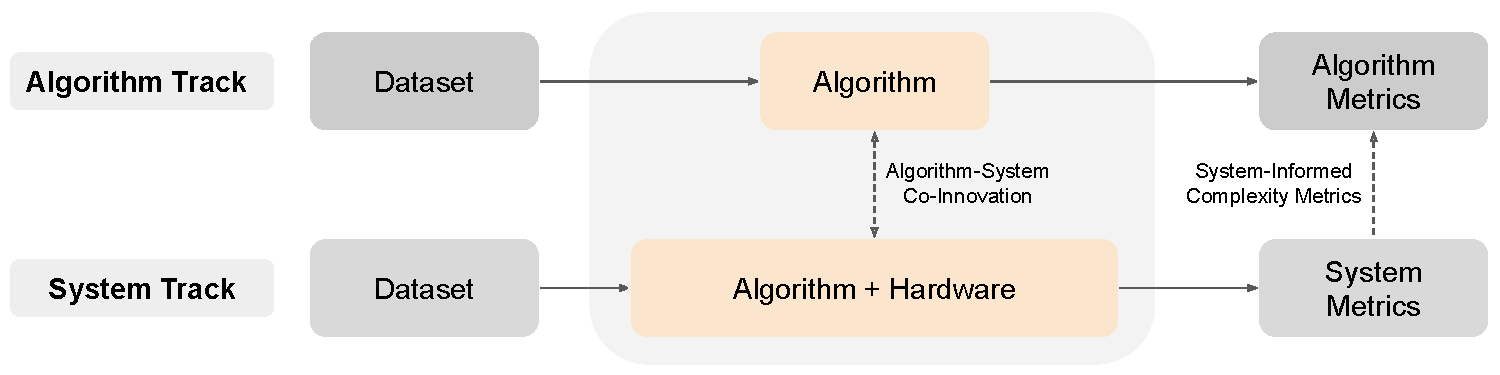
\includegraphics[width=\linewidth]{figures/tracks.pdf}
\caption{The two NeuroBench tracks: algorithms and systems. Grey boxes designate what is defined by the benchmark, and orange boxes indicate what is unique to each solution. Connecting arrows between the two tracks denote the co-innovation between the tracks and the cross-stack innovation enabled by this approach. Between algorithm and system solutions, best-performing results from each track can motivate future solutions to the other. In addition, system metrics and results can inform hardware-independent algorithmic complexity metrics. 
% \note{can augment figure with leaderboard, competition, updating versions over time}
}
\label{fig:tracks}
\end{figure}

To tackle these challenges, this article presents NeuroBench, a dual-track, multi-task benchmark framework. 
NeuroBench addresses the existing neuromorphic benchmark challenges by advancing prior work in three distinct ways. Firstly, the benchmark framework reduces assumptions regarding the specific solution being assessed, encouraging \textit{inclusive} participation of neuromorphic and non-neuromorphic approaches by utilizing general, task-level benchmarking and hierarchical metric definitions which capture key performance indicators of interest. Secondly, the NeuroBench benchmarks are associated with a common open-source benchmark harness tool which facilitates \textit{actionable} benchmark implementation and offers structure for further expansion to neuromorphic algorithm frameworks and systems. Finally, NeuroBench establishes an \textit{iterative}, community-driven initiative designed to evolve over time to ensure representation and relevance to neuromorphic research, analogous to the well-established MLPerf benchmark framework for machine learning~\cite{Reddi2020, mattson2020mlperf}.
As a whole, NeuroBench intends to align the neuromorphic research community on standard benchmarking, providing a dynamically evolving platform to ensure ongoing relevance and facilitate advancements through workshops, competitions, and a centralized leaderboard.

% JY: this should go after the previous paragraph, as the previous is tightly tied to the three points in the list
As Figure~\ref{fig:tracks} shows, the NeuroBench framework involves two tracks to enable agile algorithm and system development. As an emerging technology, neuromorphic hardware has not converged to a single platform which is commercially available, thus a large fraction of neuromorphic research explores algorithmic advancement on conventional systems which may not be optimal for performance. Thus, NeuroBench consists of an \textit{algorithm} track for hardware-independent evaluation and a \textit{system} track for fully deployed solutions. The algorithm track defines four novel benchmarks for neuromorphic methods across diverse domains, namely few-shot continual learning, computer vision, motor cortical decoding, and chaotic forecasting, and utilizes complexity metrics to analyze solution costs. Such hardware-independent benchmarking enables algorithmic exploration and prototyping, especially when simulating algorithm execution on non-neuromorphic platforms. Meanwhile, the system track defines standard protocols to measure the real-world speed and efficiency of neuromorphic hardware on benchmarks ranging from standard machine learning tasks to promising fields for neuromorphic systems, such as optimization. 

Each NeuroBench track includes defined datasets, metric and measurement methodology, and modular evaluation components to enable flexible development. Promising methods identified from the algorithm track will inform system design by highlighting target algorithms for optimization and relevant system workloads for benchmarking. The system track in turn enables optimization and evaluation of performant implementations, providing feedback to refine algorithmic complexity modeling and analysis. The interplay between the tracks creates a virtuous cycle: algorithm innovations guide system implementation, while system-level insights accelerate further algorithmic progress. This approach allows NeuroBench to advance neuromorphic algorithm-system co-design. Both the algorithm and system track will be extended and co-developed as NeuroBench continues to expand.

In the next few sections, we describe the algorithm track, including general complexity metric definitions, benchmark tasks, and common infrastructure tooling. We apply the framework to report baseline results for each algorithm benchmark, which outline unexplored research opportunities in optimizing algorithmic architectures and training of sparse, stateful models to achieve greater performance and resource efficiency. \secondrev{Then, we show baseline results established in the system track to assess neuromorphic performance across promising application workloads.}
By outlining both tracks, we provide a roadmap towards standardizing benchmark procedures in both hardware-independent and hardware dependent settings.

% % This article presents the framework of the NeuroBench benchmark suite. 
% The following Results section organizes descriptions of the algorithm track benchmark framework and its baseline results, as well as specifications of the system track benchmark framework and tasks. Further details regarding the benchmark metric formulations, task specifications, and baseline solutions can be found in the Methods section. Baseline results on NeuroBench benchmarks outline unexplored research opportunities in optimizing algorithmic architectures and training of sparse, stateful models to achieve greater performance and resource efficiency.
% As NeuroBench is intended to continually grow over time, the latest developments and opportunities to engage with the project are reported on the website.\footnote{\href{https://neurobench.ai}{https://neurobench.ai}}

\section*{Algorithm Track Benchmark Framework}
\begin{figure}[t]
            \centering
            \includesvg[width=.95\textwidth]{figures/Software_Architecture.svg}
            \caption{An overview of the NeuroBench algorithm track.}
        \label{fig:AlgTrack_SA}
    \end{figure}

The algorithm benchmark track aims to evaluate algorithms in a system-independent manner, separating algorithm performance from specific implementation details. The implementation platform can thus be ill-matched to the particular algorithm benchmark that it executes (e.g., SNN execution via dense matrix multiplication on a GPU), and the algorithm complexity and expected performance can be examined in a theoretical manner, motivating agile prototyping and functional analysis. Furthermore, minimal assumptions are made about the solutions tested, promoting inclusion of diverse algorithmic approaches.

The framework, as illustrated in Figure~\ref{fig:AlgTrack_SA}, is composed of inclusively-defined benchmark metrics, datasets and data loaders, and common harness infrastructure, shown in red. The metrics focus on assessing algorithm correctness on specific tasks as well as capturing general metrics that reflect the architectural complexity, computational demands, and storage requirements of the models. The datasets and data loaders specify the details of the tasks used for evaluation and ensure consistency across benchmarks. Finally, the harness infrastructure automates runtime execution and result output for the algorithm benchmark specified by the input interface, which consists of the user's model and customizable components for data processing and desired metrics, shown in green and orange.


% This standardized framework, as illustrated in Figure~\ref{fig:AlgTrack_SA}, allows the same algorithm to be tested across multiple platforms, with reproducible and comparable performance measurements regardless of hardware and software specifics.   In other words, the benchmarks evaluate the algorithm itself, separate from any specific implementation details. 

% Additionally, the algorithm benchmarks promote inclusion of diverse solutions by making minimal assumptions about the type of solution being tested. The benchmarks focus on assessing the correctness of the algorithm on specific tasks, as well as capturing general metrics that reflect the architectural complexity, computational demands, and storage requirements of the models. These task-centric evaluations and implementation-agnostic metrics allow for benchmarking of different algorithmic approaches to the same problem.

% The components that enable algorithm benchmarking within the standardized NeuroBench framework are shown in Figure~\ref{fig:AlgTrack_SA}. As illustrated by the red boxes, these components include defined benchmarking metrics, datasets and data loaders that specify the details of the task, and harness infrastructure to handle execution and analysis. Together, these elements allow algorithm performance to be measured in a consistent, reproducible way across algorithm categories and implementation platforms.

    \subsection*{Algorithm Track Metrics}
    The algorithm track establishes \textit{solution-agnostic} primary metrics which are generally relevant to all types of solutions, including artificial and spiking neural networks (ANNs, SNNs). Firstly, there are \textit{correctness} metrics, which measure the quality of the model predictions on the particular task, such as accuracy, mean average precision (mAP), and mean-squared error (MSE). The correctness metrics are specified per task for each benchmark. Next, there are \textit{complexity} metrics, which measure the computational demands of the algorithm. In the first iteration of the NeuroBench algorithm track, we assume a digital, time-stepped execution of the algorithm and define the following complexity metrics:

    \begin{itemize}
        \item \textbf{Footprint} -- A measure of the memory footprint, in bytes, required to represent a model, which reflects quantization, parameters, and buffering requirements. The metric summarizes (and can be further broken down into) synaptic weight count, weight precision, trainable neuron parameters, data buffers, etc. Zero weights are included, as they are distinguished in the \textit{connection sparsity} metric. 

        % \item \textbf{Model Execution Rate} -- Execution rate, in Hz, of the model computation based on forward inference passes per second, measured in the time-stepped simulation timescale. The time is correlated to real-world data time. For example, if a model is designed to process data from an event camera with 50~ms input stride, the model execution rate is 20~Hz. This metric provides intuition into the deployed real-time responsiveness of a model, as well as its computational requirements. 
        
        \item \textbf{Connection Sparsity} -- %Within the model, a measure of the relationship between the nonzero ($m$) and total potential connections ($n$), summed over each layer ($l$), $1 - \sum_l \frac{(m_l)}{(n_l)}$. 
        For a given model, the connection sparsity is the number of zero weights divided by the total number of weights, accumulated over all layers.
        0 refers to no sparsity (fully connected) and 1 refers to full sparsity (no connections). This metric accounts for deliberate pruning and sparse network architectures. 
        
        \item \textbf{Activation Sparsity} -- During execution, the average sparsity of neuron activations over all neurons in all model layers, for all timesteps of all tested samples, where 0 refers to no sparsity (i.e., all neurons are always activated), and 1 refers to the case where all neurons have a zero output.

        \item \textbf{Synaptic Operations} -- Average number of synaptic operations per model execution, based on neuron activations and the associated fanout synapses.
        % The Frequency metric lists the rate of model computations. 
        This metric is further subdivided into dense, effective multiply-accumulate, and effective accumulate synaptic operations (Dense, Eff\_MACs, Eff\_ACs). Dense accounts for all zero and nonzero neuron activations and synaptic connections, and reflects the number of operations necessary on hardware that does not support sparsity. Eff\_MACs and Eff\_ACs only count effective synaptic operations by disregarding zero activations (e.g., produced by the ReLU function in an ANN or no spike in an SNN) and zero connections, thus reflecting operation cost on sparsity-aware hardware. Synaptic operations with non-binary activation are considered multiply-accumulates (MACs), while those with binary activation are considered accumulates (ACs).
    \end{itemize}

    Footprint and connection sparsity are classified as \textit{static metrics}, which can be analytically determined from the model only. Activation sparsity, synaptic operations, and correctness are classified as \textit{workload metrics}, which are dependent on execution or simulation of the model based on the benchmark data.

    \revision{In addition to the above complexity metrics, the algorithm track proposes to define \textit{Model Execution Rate}, corresponding to the rate, in Hz, at which the model's forward inference pass needs to be executed. For example, if a model is designed to process data from an event camera with a 50 ms input stride, the model execution rate is 20 Hz. The execution rate is a critical feature of the algorithm which provides intuition into the tradeoff between latency and computational footprint of a \textit{deployed} model, and is reported directly by the solution designer in benchmark results since it neither needs to be calculated nor extracted from the model or its outputs.}

    %\revision{In addition to the complexity metrics, the algorithm track defines the \textbf{Model Execution Rate} numeric, which is the execution rate, in Hz, of the model computation based on forward inference passes per second, measured in the time-stepped simulation timescale. For example, if a model is designed to process data from an event camera with 50 ms input stride, the model execution rate is 20 Hz. The execution rate is a critical feature of the algorithm which provides intuition into the deployed real-time responsiveness and computational requirements of a model, and is reported directly by the solution designer in benchmark results since it neither needs to be calculated nor extracted from the model or its outputs.}
    
    The complexity metrics are measured independently of the underlying hardware and therefore do not explicitly correlate with post-deployment latency or energy consumption. However, they provide valuable insight into algorithm performance and resource requirements, enabling high-level comparison and facilitating prototyping. For instance, the execution rate and number of synaptic operations can be taken together to estimate the speed and dynamic power of a model deployed to certain hardware, and the footprint and connection sparsity can be used to proxy hardware resource utilization. %and static power.

    Furthermore, the algorithm track can be extended with \textit{solution-specific} secondary metrics, which can offer deeper insights by using information specific to particular types of solutions. For example, for algorithms geared towards analog hardware, noise robustness is an important solution-specific metric. In addition, approaches with complex neuron dynamics may warrant measuring the overall complexity of a neuron update (i.e., type and counts of operations necessary to simulate the update), which can be combined with the total number of neuron updates in a model pass to calculate the cost of state updates. Such solution-specific metrics are expected to be community-driven and will be included in future NeuroBench algorithm track releases.


    % JY: Moved this to after the benchmarks
    % \paragraph{Limitations and Future Extensions.}
    % The first-iteration algorithm track metrics are currently restricted to the assumption of a digital time-stepped execution of the algorithm. 
    % Complexity analysis of digital time-stepped prototypes can be used as an intermediate step for solutions intended for analog or continuous time deployment, but the metric measurements are not yet defined for such execution.
    % Informed by further benchmark implementations, future versions of NeuroBench will extend inclusiveness by expanding measurement protocols to include such algorithms.

    % The synaptic operations metric, intended to capture the model computation cost, currently does not account for neuron updates. The dynamics of neuron models, including mechanisms such as leakage and reset, can vary heavily in complexity. However, the number and type of operations of neuron updates, as well as their overall costs, depend on arithmetic or circuit implementation, and thus are not accounted for in the broader algorithmic complexity metrics. Solution-specific metrics which assume a particular implementation platform, which have been defined previously~\cite{Lemaire_2023}, can be used to estimate neuron update costs. These can be combined with the total number of neuron updates per model computation in order to measure neuron operation complexity during evaluation.

    % Data pre- and post-processing costs are also not yet captured in the NeuroBench algorithm track metrics. Such costs are, however, captured in the deployed metrics of the system track, which accounts for data processing hardware as part of the overall system during performance and efficiency measurements. Data processing metrics will be added as a separate complexity category for the algorithm track in the future.


    
    
    % Data pre- and post-processing costs are not captured in the algorithm track due to the system-specific reliance of data manipulation (e.g., in-sensor data processing, such as in spiking sensors~\cite{anumula2018feature, Lichtsteiner_etal08_128x120}). 
    % Such costs are, however, captured in the deployed metrics of the system track, which accounts for data processing hardware as part of the overall system during performance and efficiency measurements.
\subsection*{Algorithm Track Benchmarks}

    The v1.0 iteration of the NeuroBench algorithm track includes four benchmarks for neuromorphic computing research. The benchmarks were chosen by the NeuroBench community to capture key ongoing challenges for neuromorphic algorithm design. The list of tasks highlights features which are relevant to neuromorphic research interests: few-shot continual learning, object detection utilizing the high dynamic range and temporal resolution of event cameras, sensorimotor decoding based on cortical signals, and low-dimensional predictive modeling useful for prototyping resource-constrained networks that are suitable for small mixed-signal systems.
    % The benchmark tasks and baselines were produced by working groups comprised of various industry and academic researchers within the NeuroBench community. 
    Benchmark tasks are listed below and summarized in Table \ref{tab:alg_benchmarks}. Detailed specifications of benchmark tasks are provided in the Methods section. 
    
    % \begin{table}[t]
%         \centering
%         { \renewcommand{\arraystretch}{1.2}
%         \begin{tabular}{|c|c|c|p{0.23\linewidth}|}
%         \hline
%              Task & Dataset & Correctness metric(s) & Task description  \\\hline
%              Keyword FSCIL & MSWC~\cite{mazumder21mswc} & Accuracy & Few-shot, continual learning of keyword classes. \\\hline
%              Event Camera Object Detection & Prophesee 1MP Automotive~\cite{Perot2020}  & COCO mAP & Detecting automotive objects from event-sensor video.  \\\hline
%              Motor Prediction & Primate Reaching~\cite{makin-dataset} & R$^2$ & Predicting fingertip velocity from cortical data.  \\\hline
%              Chaotic Function Prediction & Mackey-Glass time series~\cite{mackey1977oscillation} & sMAPE & Autoregressive modeling of chaotic functions.  \\\hline
              
%         \end{tabular}
%         }
%         \caption{NeuroBench algorithm track v1.0 benchmarks.}
%         \label{tab:alg_benchmarks}
%     \end{table}

\begin{table}[t]
    \centering
    \renewcommand{\arraystretch}{1.3}
    \begin{tabular}{lllm{0.23\linewidth}}
        \thickhline
        Task & Dataset & Correctness metric & Task description  \\\hline
        Keyword FSCIL & MSWC~\cite{mazumder21mswc} & Accuracy & Few-shot, continual learning of keyword classes. \\\hline
        Event Camera Object Detection & Prophesee 1MP Automotive~\cite{Perot2020}  & COCO mAP & Detecting automotive objects from event camera video.  \\\hline
        NHP Motor Prediction & Primate Reaching~\cite{makin-dataset} & R$^2$ & Predicting fingertip velocity from cortical recordings.  \\\hline
        Chaotic Function Prediction & Mackey-Glass time series~\cite{mackey1977oscillation} & sMAPE & Autoregressive modeling of chaotic functions.  \\\thickhline
    \end{tabular}
    \caption{NeuroBench algorithm track v1.0 benchmarks.}
    \label{tab:alg_benchmarks}
\end{table}


    
    \begin{itemize}
        \item \textbf{Keyword Few-Shot Class-Incremental Learning (FSCIL)} --
        Learning new tasks from a small amount of experiences while retaining knowledge of prior tasks is a hallmark of biological intelligence and a long-standing goal of general AI~\cite{kudithipudi22biological}. It is especially a key challenge to endow edge devices with the ability to adapt to their environments and users. This benchmark thus evaluates the capacity of a model to successively incorporate new keywords over multiple sessions (class-incremental), with only a handful of samples from the new classes to train with (few-shot). The FSCIL task is a recently established benchmark in the computer vision domain~\cite{tao2020fscil}, but it has not yet been adapted to other data modalities. Aligning with a neuromorphic interest in temporal data modalities, this benchmark introduces a FSCIL task with streaming audio data using the large Multilingual Spoken Word Corpus (MSWC)~\cite{mazumder21mswc} keyword classification dataset. The task is designed to be approached in two phases: pre-training and incremental learning. First, for pre-training, a set of 100 words spanning 5 base languages (English, German, Catalan, French, Kinyarwanda) with 500 training samples each are made available to train an initial model. Next, for incremental learning, the model undergoes 10 successive sessions to learn words from 10 new languages (Persian, Spanish, Russian, Welsh, Italian, Basque, Polish, Esparanto, Portuguese, Dutch) in a few-shot learning scenario. Each incremental session adds 10 words of the corresponding session language with only 5 training samples available per word. After each session, the model is tested in classification accuracy on all prior learned classes, including the 100 base pre-training classes and the few-shot-learned classes,
        %, with 100 test samples per class
        therefore evaluating the FSCIL solution on its ability to learn new classes while retaining knowledge about the previously learned ones. Each session learns a new language, for a total knowledge base of 200 keywords by the end of the benchmark.

        
        \item \textbf{Event Camera Object Detection} --
        Object detection is a widely-used computer vision task with applications in robotics, autonomous driving, and surveillance. Such scenarios at the edge may require high energy efficiency and real-time performance, which can be achieved via event-based vision sensors~\cite{Gallego2022}. The event camera object detection benchmark uses the Prophesee 1 Megapixel automotive detection dataset~\cite{Perot2020}, a large labeled object detection dataset with over 15 hours of event camera video from the front of a car driving in various scenarios. Predetermined training, validation, and testing splits include \SI{11.2}{\hour}, \SI{2.2}{\hour}, and \SI{2.2}{\hour} of recording, respectively. Pedestrian, two-wheeler, and car object classes are used in evaluation, and correctness is measured using COCO mean average precision (mAP)~\cite{LinCOCO_2014}.
        
        \item \textbf{Non-human Primate (NHP) Motor Prediction} --
        Studying models which can accurately replicate features of biological computation presents opportunities in understanding sensorimotor behavior and developing closed-loop methods for future robotic agents. It also is foundational to the development of wearable or implantable neuro-prosthetic devices that can accurately generate motor activity from neural or muscle signals. This benchmark utilizes a dataset consisting of multi-channel recordings from the sensorimotor cortex of two non-human primates (NHP Indy and NHP Loco) during reaching movements, along with corresponding fingertip motion of the reach~\cite{makin-dataset}. Six total sessions are included from the dataset, for a total of 8712 seconds of data. The task is to train a model to predict the two-dimensional components of finger velocity using recent neural data. The sessions are treated independently (i.e., models are trained separately for each session), and the data is split to allow the first 75\% for training and validation and the last 25\% for evaluation. Correctness of the predictions is evaluated by the coefficient of determination ($R^{2}$) score against the true finger velocity targets, averaged over all six sessions.
        
        \item \textbf{Chaotic Function Prediction} --
        The real-world data benchmarks presented thus far are high-dimensional and can require large networks to achieve high accuracy, raising challenges for solution types with limited I/O support and network capacity, such as mixed-signal edge prototype solutions. To address this, we include a synthetic benchmark based on prediction of one-dimensional Mackey-Glass time series~\cite{mackey1977oscillation}, which can be effectively tackled by smaller networks. Mackey-Glass has been widely adopted as a benchmark for evaluating temporal predictors, including neuromorphic models~\cite{jaeger2004harnessing, mukhopadhyay2020learning, chilkuri2021parallelizing}. The task involves prediction of the next timestep value $f(t+\Delta t)$ given the current timestep value $f(t)$. 
        The model is trained and validated using the first half of the time series, during which the ground truth state $f(t)$ are supplied to the model to predict the next timestep $f'(t+\Delta t)$.
        During the evaluation, the model uses its prior prediction $f'(t)$ to generate each next value $f'(t+\Delta t)$, autoregressively forecasting the second half of the time series.
        Correctness is measured using symmetric mean absolute percentage error (sMAPE) of the generated time series against the target time series, a standard metric in forecasting~\cite{MAKRIDAKIS202054}.
        The benchmark includes a set of 14 Mackey-Glass time series, which vary by the equation parameter $\tau$, the delay constant. Lyapunov time $(L)$, the expected predictability timescale for chaos~\cite{gilpin2023largescale}, is used as the time unit for each time series. The total length of each series is 20 Lyapunov times, and 75 points are sampled per Lyapunov time ($\Delta t$ = $L/75$).

    \end{itemize}

\subsection*{Algorithm Track Benchmark Harness}
    The NeuroBench algorithm benchmarks are wrapped in a harness which standardizes the benchmark interfaces. The harness provides benchmark users with a consistent framework for loading data, processing data and model outputs, and calculating and reporting metrics, thereby ensuring fair and standard comparisons of the results. It is built with straightforward interfaces which are designed to be extended with new frameworks, algorithms, and tasks. The benchmark harness is open-source for use and development (\url{https://github.com/NeuroBench/neurobench}).
    %\footnote{\url{https://github.com/NeuroBench/neurobench}}
    
    The components of the algorithm benchmark harness are summarized in Figure~\ref{fig:AlgTrack_SA}.
    % Note that the execution flow currently assumes a digital time-stepped execution of the algorithm, but can be extended to continuous values such as in analog design in the future
    \textit{Datasets} are loaded in a common format and pass through \textit{Processors} to be pre-processed. The \textit{Model} generates predictions based on the processed data, and \textit{Accumulators} post-process the predictions, for instance to accumulate spikes and transform to labels. Static metrics of algorithm footprint and connection sparsity are calculated via model analysis, while metrics of correctness, activation sparsity, and synaptic operations are calculated using predictions and model execution traces. For benchmark users, task evaluation simply involves utilizing the existing dataloaders, processors, and metrics within the harness and wrapping their own code to fit the standard interfaces.
 
    Currently, the harness and all baseline models are built using PyTorch~\cite{paszke19pytorch} or frameworks based on it, such as snnTorch~\cite{eshraghian2021training} and SpikingJelly~\cite{SpikingJelly}. Due to its modular structure and simple interfaces, the harness can grow to be compatible with further neuromorphic tools such as Lava~\cite{lava} and Fugu~\cite{aimone2019composing}.
    Furthermore, it also supports the extension of data and metric pipelines in order to implement additional benchmark tasks. \revision{Widely validated benchmarks in keyword~\cite{warden2018speech} and gesture classification~\cite{Amir_etal17_lowpowe}, which are foundational in neuromorphic and conventional research~\cite{blouw2019, Cramer_2022, fang2021incorporating, massa2021efficient}, have been incorporated into the harness to complement the novel tasks in the NeuroBench v1.0 suite.} Any novel or existing benchmarks can make use of the harness infrastructure for open reproducibility, and also to garner interest in the community towards long-term task support and appearance in NeuroBench-affiliated leaderboards and challenge events.
    % As NeuroBench is a community-driven project, we welcome interested developers to contribute to the benchmark harness through the associated code repository. 

\subsubsection*{Algorithm Track Limitations and Further Extensions}

Before diving into the baseline results, it is worth discussing several possible improvements to the NeuroBench algorithm track framework in its current form. Specifically, the initial iteration of metrics is restricted to the assumption of digital, time-stepped algorithm execution. While complexity analysis of such prototypes can serve as an intermediate step for solutions intended for analog or continuous time deployment, the metric measurements are not yet defined for those execution settings. Informed by further benchmark implementations, future versions of NeuroBench will extend inclusiveness by expanding measurement protocols to include such algorithms.

\revision{Furthermore, the synaptic operations metric, intended to capture model computation cost, currently does not account for neuron updates. The dynamics of neuron models, including mechanisms like leakage and reset, can vary heavily in complexity. However, counting the number and type of operations from neuron updates, as well as estimating their overall costs, depends on the specific arithmetic or circuit implementation. Thus, they are not accounted for in the broader algorithmic complexity metrics. The algorithmic metric framework can be extended with solution-specific metrics that assume a particular implementation platform to estimate neuron update costs, which have been previously defined~\cite{Lemaire_2023}. These estimates can then be combined with the total number of neuron updates per model computation to measure overall network operation complexity during evaluation.}

% Solution-specific metrics that assume a particular implementation platform, as have been defined previously~\cite{Lemaire_2023}, can be used to estimate neuron update costs. These estimates can then be combined with the total number of neuron updates per model computation to measure overall neuron operation complexity during evaluation.

Data pre- and post-processing can also amount to significant costs not yet captured in the NeuroBench algorithm track metrics. Such costs are, however, captured in the deployed metrics of the system track, which accounts for data processing hardware as part of the overall system during performance and efficiency measurements. Data processing metrics will be added as a separate complexity category for the algorithm track benchmark in the future.

The v1.0 algorithm track benchmark suite is also intended to expand in the future. This could include covering further data modalities such as inertial measurement unit (IMU) sensing~\cite{fra22har} and extending to closed-loop sensorimotor tasks to demonstrate embodied intelligence. As with the initial benchmarks, further tasks will undergo approval and development by the open NeuroBench community before being included in a future versioned benchmark suite.

% Several improvements are possible on the benchmark metrics, tasks and harness. The first-iteration algorithm track metrics are currently restricted to the assumption of a digital time-stepped execution of the algorithm. Complexity analysis of digital time-stepped prototypes can be used as an intermediate step for solutions intended for analog or continuous time deployment, but the metric measurements are not yet defined for such execution. Informed by further benchmark implementations, future versions of NeuroBench will extend inclusiveness by expanding measurement protocols to include such algorithms.

% Furthermore, the synaptic operations metric, intended to capture the model computation cost, currently does not account for neuron updates. The dynamics of neuron models, including mechanisms such as leakage and reset, can vary heavily in complexity. However, the number and type of operations of neuron updates, as well as their overall costs, depend on arithmetic or circuit implementation, and thus are not accounted for in the broader algorithmic complexity metrics. Solution-specific metrics which assume a particular implementation platform, which have been defined previously~\cite{Lemaire_2023}, can be used to estimate neuron update costs. These can be combined with the total number of neuron updates per model computation in order to measure neuron operation complexity during evaluation.

% Data pre- and post-processing can amount to be significant. These costs are also not yet captured in the NeuroBench algorithm track metrics. Such costs are, however, captured in the deployed metrics of the system track, which accounts for data processing hardware as part of the overall system during performance and efficiency measurements. Data processing metrics will be added as a separate complexity category for the algorithm track in the future.

% The v1.0 algorithm track benchmark suite is also intended to be expanded in the future, for instance covering further data modalities such as inertial measurement unit (IMU) sensing~\cite{fra22har} and extending to closed-loop sensorimotor tasks to demonstrate embodied intelligence. As with the initial benchmarks, further tasks will undergo approval and development by the open NeuroBench community to be included in a future versioned benchmark suite.    
\subsection*{Algorithm Track Baseline Results}

% TODO if time: update section structure clarity with bolded presentation of main points

% Given our first itereation of the algorithmic track, we report baseline algorithm performance on each of the benchmarks using model architectures ranging from ANNs commonly used in deep-learning, to SNNs and reservoir networks. Each benchmark is evaluated with two significantly differing algorithm baselines, and we extract baseline comparisons, trends, and motivations towards future research. 

In our first iteration of the algorithmic track, we report baseline algorithm performance on each benchmark using various model architectures, including artificial neural networks commonly used in deep learning, spiking neural networks, and reservoir networks. We evaluate each benchmark with two substantially different algorithm baselines. From these evaluations, we extract baseline comparisons, identify trends, and uncover motivations for future research. Except for the event camera object detection task, each benchmark utilizes a novel data split, and all tasks use novel metric measurement. The presented baselines are a snapshot of the solution search space and will be starting points for leaderboards, thereby calling for further research to push the state of the art for each task. Detailed specifications of each of the baselines can be found in the Methods section.

    \subsubsection*{Keyword FSCIL}
    % \begin{table}[h]
% \centerline{
% \renewcommand{\arraystretch}{1.2}
% \begin{tabular}{|c|c|c|c|c|c|ccc|}
% \hline
% \multirow{2}{*}{Baseline} &
%   \multirow{2}{*}{\begin{tabular}[c]{@{}c@{}}Base\\ Accuracy\end{tabular}} &
%   \multirow{2}{*}{\begin{tabular}[c]{@{}c@{}}Footprint\\ (bytes)\end{tabular}} &
%   \multirow{2}{*}{\begin{tabular}[c]{@{}c@{}}Frequency\\ (Hz)\end{tabular}} &
%   \multirow{2}{*}{\begin{tabular}[c]{@{}c@{}}Connection\\ Sparsity\end{tabular}} &
%   \multirow{2}{*}{\begin{tabular}[c]{@{}c@{}}Activation\\ Sparsity\end{tabular}} &
%   \multicolumn{3}{c|}{SynOps (per sample)} \\ \cline{7-9} 
%         &       &          &    &     &       & \multicolumn{1}{c|}{Dense}    & \multicolumn{1}{c|}{Eff\_MACs} & Eff\_ACs \\ \hline
% M5 ANN & 97.36\% & $6.03 \times 10^6$ & 1 & 0.0 & 0.856 & \multicolumn{1}{c|}{$2.44 \times 10^9$} & \multicolumn{1}{c|}{$1.16 \times 10^8$}  & 0 \\ \hline
% SNN  & 93.77\% & $1.35 \times 10^7$ & 200 & 0.0 & 0.899 & \multicolumn{1}{c|}{$5.13 \times 10^9$} & \multicolumn{1}{c|}{0.0}  & $6.08 \times 10^8$ \\ \hline
% \end{tabular}
% }
% \caption{Baseline results for the keyword few-shot class-incremental learning task.}
%     \label{tab:FSCIL_resuls}
% \end{table}

% \begin{table}[ht]
% \centerline{
% \renewcommand{\arraystretch}{1.3}
% \begin{tabular}{c|cccccccc} \thickhline
% \multirow{2}{*}{Baseline} &
%   \multirow{2}{*}{\begin{tabular}[c]{@{}c@{}}Pre-training\\ Accuracy\end{tabular}} &
%   \multirow{2}{*}{\begin{tabular}[c]{@{}c@{}}Footprint\\ (bytes)\end{tabular}} &
%   \multirow{2}{*}{\begin{tabular}[c]{@{}c@{}}Frequency\\ (Hz)\end{tabular}} &
%   \multirow{2}{*}{\begin{tabular}[c]{@{}c@{}}Connection\\ Sparsity\end{tabular}} &
%   \multirow{2}{*}{\begin{tabular}[c]{@{}c@{}}Activation\\ Sparsity\end{tabular}} &
%   \multicolumn{3}{c}{SynOps (per sample)} \\ \cline{7-9} 
%         &       &          &    &     &       & \multicolumn{1}{c}{Dense}    & \multicolumn{1}{c}{Eff\_MACs} & Eff\_ACs \\ \hline
% M5 ANN & 97.36\% & $6.03 \times 10^6$ & 1 & 0.0 & 0.856 & \multicolumn{1}{c}{$2.44 \times 10^9$} & \multicolumn{1}{c}{$1.16 \times 10^8$}  & 0 \\ 
% SNN  & 93.77\% & $1.35 \times 10^7$ & 200 & 0.0 & 0.899 & \multicolumn{1}{c}{$5.13 \times 10^9$} & \multicolumn{1}{c}{0}  & $6.08 \times 10^8$ \\ \thickhline
% \end{tabular}
% }
% \caption{Baseline results for the keyword few-shot class-incremental learning task. Here, accuracy on the base 100 classes is reported. Accuracy across incremental sessions is shown in Figure~\ref{fig:mswc_acc_per_session}. \TODO{Update the synops with the correct synops} \JY{? Change to Compute Frequency, SynOps per compute}}
%     \label{tab:FSCIL_resuls}
% \end{table}



\begin{table}[ht]
\centerline{
\renewcommand{\arraystretch}{1.3}
\begin{tabular}{c|cccccccc} \thickhline
\multirow{2}{*}{Baseline} &

  \multirow{2}{*}{\begin{tabular}[c]{@{}c@{}}Accuracy\\ (Base / Session Avg)\end{tabular}} &
  \multirow{2}{*}{\begin{tabular}[c]{@{}c@{}}Footprint\\ (bytes)\end{tabular}} &
  \multirow{2}{*}{\begin{tabular}[c]{@{}c@{}}Model Exec.\\ Rate (Hz)\end{tabular}} &
  \multirow{2}{*}{\begin{tabular}[c]{@{}c@{}}Connection\\ Sparsity\end{tabular}} &
  \multirow{2}{*}{\begin{tabular}[c]{@{}c@{}}Activation\\ Sparsity\end{tabular}} &
  \multicolumn{3}{c}{SynOps (per model exec.)} \\ \cline{7-9} 
        &       &          &    &     &       & \multicolumn{1}{c}{Dense}    & \multicolumn{1}{c}{Eff\_MACs} & Eff\_ACs \\ \hline
M5 ANN & (97.09\% / 89.27\%) & $6.03 \times 10^6$ & 1 & 0.0 & 0.783 & \multicolumn{1}{c}{$2.59 \times 10^7$} & \multicolumn{1}{c}{$7.85 \times 10^6$}  & 0 \\ 
SNN  & (93.48\% / 75.27\%) & $1.36 \times 10^7$ & 200 & 0.0 & 0.916 & \multicolumn{1}{c}{$3.39 \times 10^6$} & \multicolumn{1}{c}{0}  & $3.65 \times 10^5$ \\ \thickhline
\end{tabular}
}
\caption{Baseline results for the keyword few-shot class-incremental learning task. Base accuracy refers to accuracy on the 100 base classes after pre-training while session average accuracy is the average accuracy over all sessions for the corresponding prototypical baseline. The detailed accuracy per session for the different baselines are shown in Figure~\ref{fig:mswc_acc_per_session}.}
    \label{tab:FSCIL_results}
\end{table}



% WEIGHT CONSOLIDATION RESULTS

% \begin{table}[ht]
% \centerline{
% \renewcommand{\arraystretch}{1.3}
% \begin{tabular}{c|cccccccc} \thickhline
% \multirow{2}{*}{Baseline} &
%   \multirow{2}{*}{\begin{tabular}[c]{@{}c@{}}Pre-training\\ Accuracy\end{tabular}} &
%   \multirow{2}{*}{\begin{tabular}[c]{@{}c@{}}Footprint\\ (bytes)\end{tabular}} &
%   \multirow{2}{*}{\begin{tabular}[c]{@{}c@{}}Model Exec.\\ Rate (Hz)\end{tabular}} &
%   \multirow{2}{*}{\begin{tabular}[c]{@{}c@{}}Connection\\ Sparsity\end{tabular}} &
%   \multirow{2}{*}{\begin{tabular}[c]{@{}c@{}}Activation\\ Sparsity\end{tabular}} &
%   \multicolumn{3}{c}{SynOps (per model exec.)} \\ \cline{7-9} 
%         &       &          &    &     &       & \multicolumn{1}{c}{Dense}    & \multicolumn{1}{c}{Eff\_MACs} & Eff\_ACs \\ \hline
% M5 ANN & 97.36\% & $6.03 \times 10^6$ & 1 & 0.0 & 0.856 & \multicolumn{1}{c}{$2.59 \times 10^7$} & \multicolumn{1}{c}{$5.75 \times 10^6$}  & 0 \\ 
% SNN  & 93.77\% & $1.35 \times 10^7$ & 200 & 0.0 & 0.916 & \multicolumn{1}{c}{$3.39 \times 10^6$} & \multicolumn{1}{c}{0}  & $3.65 \times 10^5$ \\ \thickhline
% \end{tabular}
% }
% \caption{Baseline results for the keyword few-shot class-incremental learning task. Here, accuracy after pre-training on the base 100 classes is reported. Accuracy across incremental sessions is shown in Figure~\ref{fig:mswc_acc_per_session}.}
%     \label{tab:FSCIL_results}
% \end{table}

    The keyword FSCIL task has an ANN and SNN baseline, using different model architectures:
    
    \begin{itemize}
        \item \textbf{M5 ANN} -- The ANN baseline uses a tuned version of the M5 deep convolutional network architecture~\cite{dai2016deep}, with samples pre-processed into Mel-frequency cepstral coefficients (MFCC). The network contains four successive convolution-normalization-pooling layers, followed by a readout fully-connected layer. Each model execution (forward pass) uses the data from the full pre-processed sample, and convolution kernels are applied over the temporal dimension of the samples. This is reported as a 1~Hz model execution rate.
        % Convolutional kernels are applied over the temporal dimension of the samples. 

        \item \textbf{SNN} -- The SNN baseline uses a recurrent SNN with adaptive leaky integrate-and-fire (LIF) neurons and heterogeneous time constants~\cite{bittar22surrogate}. The SNN consists of two recurrent adaptive LIF layers and one linear output layer.
        Audio samples are pre-processed to binary spike trains using Speech2Spikes~\cite{stewart23speech2spikes}, which relies on a Mel Spectrogram with the same parameters as the MFCC of the ANN baseline. Each input timestep to the model represents 5~ms of audio data, thus the model has a 200~Hz model execution rate. Output neuron activations are summed over time to produce the word class prediction.
    \end{itemize}

    % \begin{figure}[h]
    %             \centering
    %             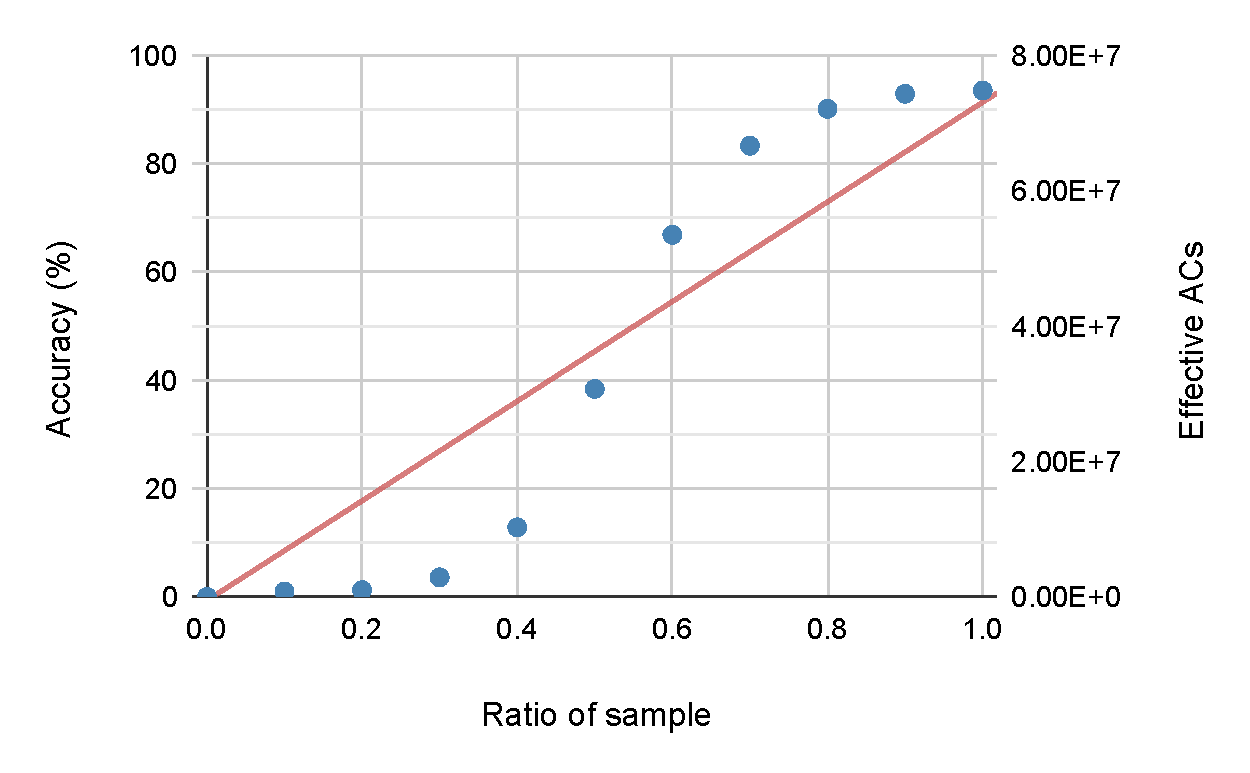
\includegraphics[width=.70\textwidth]{figures/snn_acc_compute_time.pdf}
    %             \caption{Test accuracy (blue) and aggregated effective ACs (red) of SNN on base classes using only the first portions of the keyword sample.}
    %         \label{fig:snn_acc_time}
    %     \end{figure}

% a base session with fixed classes, each with abundant training data, is used to train an initial model. Then, successive incremental training sessions introduce new classes in a few-shot learning scenario. In each session, only the current session classes are available to the model for training. After each incremental training session, the model is evaluated on all previously seen classes, including the base classes. Therefore, the model has to learn new classes while retaining knowledge about the previously learned ones. 

    % The keyword FSCIL task first uses a base dataset consisting of 100 base classes with abundant training data to pre-train models before proceeding with incremental learning on 100 extra classes. 
    After pre-training using standard batched training, the ANN and SNN baseline networks reach high accuracies on the base classes of 97.09\% and 93.48\%, respectively.
    % \red{The SNN solution, including the pre-processing, processes one input timestep at a time with a frequency of 200~Hz, compared to the ANN which requires a full one second sample to pass through the model. While the number of effective operations per-sample is lower for the ANN baseline, the SNN distributes computation temporally over 200 timesteps, thus its effective operations per model execution is one order of magnitude lower ($3.65 \times 10^5$).}
    As reported by the model execution rate metric, the SNN baseline computes each sample over 200 passes, using an order of magnitude fewer effective AC synaptic operations compared to the ANN baseline's effective MACs per model execution.
    Considering both the model execution rate and synaptic operation metrics, the number of aggregated ACs over the length of the sample ($200 * 3.65 \times 10^5 = 7.30 \times 10^7$) exceeds the Dense and effective MAC operations necessary for the ANN baseline, which spatially flattens the sample and processes it in one model execution.
    However, outside of the static-length keyword classification scenario, the low-cost per-execution temporal processing of SNNs can enable efficient, always-on, high-frequency prediction capabilities in deployed continuous audio recognition scenarios. 

    % Furthermore, the temporal processing of the SNN has capabilities to produce predictions before the sample is completed. 
    % Figure~\ref{fig:snn_acc_time} demonstrates that the SNN reaches 90\% accuracy using the first 80\% of the sample. Moreover, the number of aggregated effective ACs grows as a linear function of the sample ratio, demonstrating a compute reduction corresponding to the early prediction. Further research in online neuromorphic methods for fast time-to-prediction and compute-accuracy trade-offs\cite{jeffares2022spikeinspired} is enabled by the benchmark data features (see Methods section).
    

    \begin{figure}[ht]
                \centering
                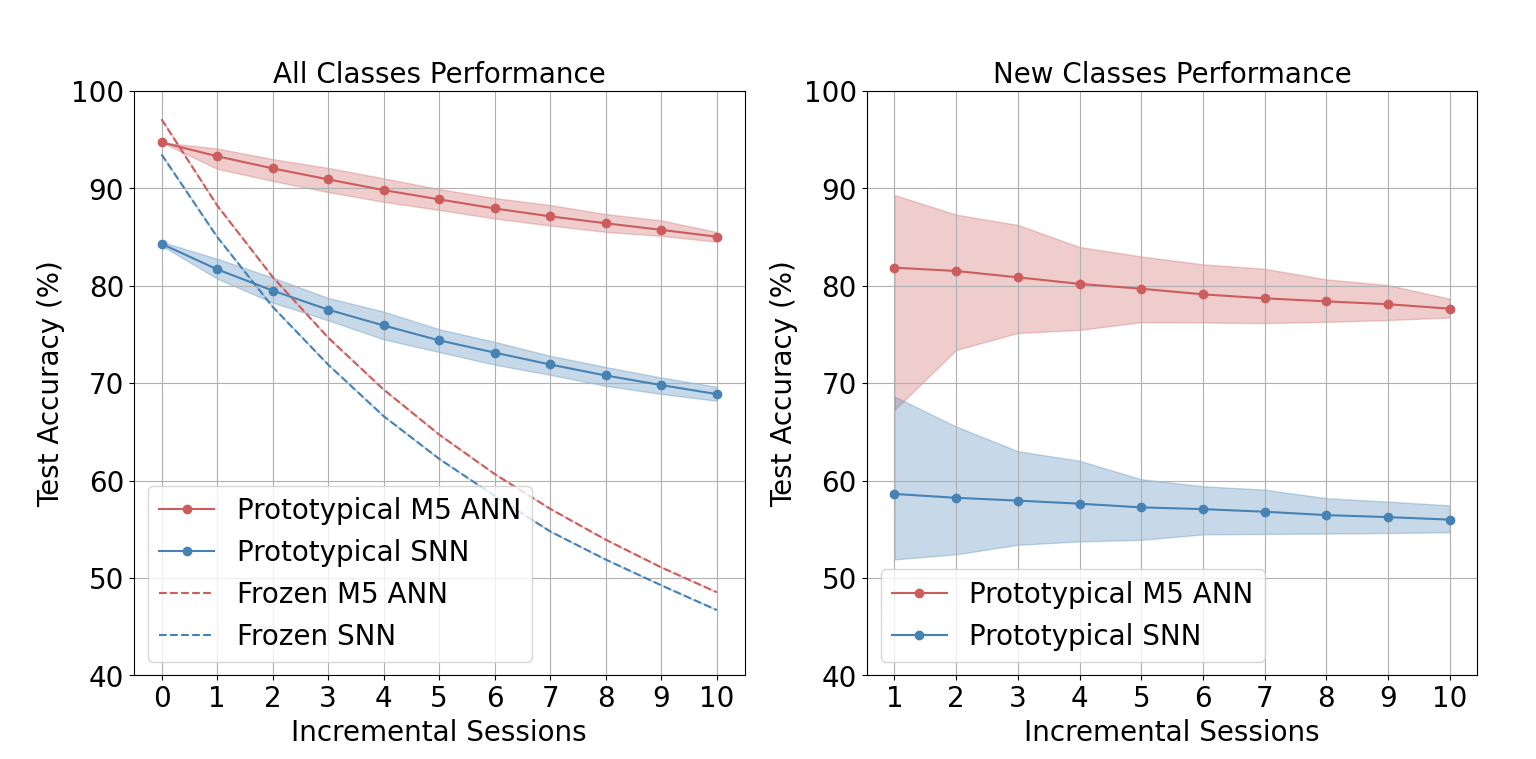
\includegraphics[width=\textwidth]{figures/FSCIL_proto.png}
                \caption{Test accuracy per session on the keyword FSCIL task for prototypical and frozen baselines, with the accuracy on both base classes and incrementally-learned classes (left), and accuracy on all incrementally-learned classes only (right). Incremental session 0 refers to the accuracy on base classes after pre-training only. Shaded area represents 5$^{th}$ and 95$^{th}$ percentile on 100 runs. Frozen baselines with no adaptation do not learn incremental classes and thus have a fixed 0\% accuracy for New Classes Performance. }
            \label{fig:mswc_acc_per_session}
        \end{figure}


    % For the incremental learning portion of the task, 10 successive sessions, each representing a new language, are presented to the model. Each session contains 10 new classes with 5 samples each (10-way 5-shot learning). This set-up 

% NEW VERSION WITH PROTOTYPES METHOD:

    % The 10-way, 5-shot class-incremental learning per incremental session poses the challenge of learning new classes while avoiding catastrophic forgetting, especially with the limited number of samples for new classes. We therefore present two reference solutions for both the ANN and SNN baselines: a \textbf{frozen} baseline with no weight updates in the incremental learning phase and a \textbf{prototypical} baseline that employs class prototypes~\cite{snell2017prototypical} for incremental learning. 
    % The frozen ANN and SNN have 0\% accuracy on incremental classes, and serve as reference for models which have no learning, but also no catastrophic forgetting of prior classes. 

    % In prototypical networks~\cite{snell2017prototypical}, all classes are associated with a \textit{prototype}, which is the average feature embedding, produced by the network before the readout classifier layer, over all training samples for each class. During inference, input samples are classified as the class corresponding to the prototype with the lowest squared Euclidean distance to the sample's embedding. Since computing this distance is equivalent to an affine operation on the feature embeddings~\cite{snell2017prototypical}, the prototypical network classifier can be expressed as a standard linear readout layer defined with respect to the prototype of each class. Thus, the final model consists of a prototype classifier output layer following the feature extracting hidden layers.

    % Although the original work on prototypical networks suggests a specific approach to train the feature extractor network~\cite{snell2017prototypical}, we employ standard pre-training with end-to-end backpropagation to enable high base class accuracy. After pre-training, the readout classifier layer is dropped, and the base classes prototypes and prototype layer are computed a-posteriori based on features from the hidden layers of the pre-trained network. This allows for common readout classification for base and incremental classes, however, it comes with an accuracy loss for base classes as the feature extraction in hidden layers is not trained with the classifier. 

    % The prototypical network approach is simple and computationally efficient, as no hyperparameters are used and parameters are not optimized, but instead calculated directly. 
    % Also, the prototypical evaluation method does not affect model complexity, as the prototypical classifier directly substitutes the default readout layer. Thus, the complexity results in Table~\ref{tab:FSCIL_results} empirically apply to both the frozen and prototypical models.

    % JY: compressed details from prior 4 paragraphs into this single paragraph, also compressed the following paragraphs
    We present two approaches for the incremental stage for both the ANN and SNN baselines. The \textit{frozen} models are locked after pre-training on base classes and have 0\% accuracy on all new incremental classes, providing a reference for models with no learning or catastrophic forgetting of prior classes. The \textit{prototypical} models employ a prototypical network~\cite{snell2017prototypical} for incremental learning, which is a feature-based clustering approach that can be implemented with a simple linear readout layer on top of the pre-trained network backbone. Prototypical weights and biases of prior and incremental classes are directly defined based on the average features of the corresponding class and directly substitute pre-trained readout layer parameters.  The complexity results in Table~\ref{tab:FSCIL_results} thus empirically apply to both the frozen and prototypical models.
    
    The test accuracy for the baseline models over all sessions, as well as the test accuracy on only the new incrementally-learned classes, are shown in Figure~\ref{fig:mswc_acc_per_session}.
    Using prototypical networks, the ANN model reaches 89.27\% accuracy on average over all sessions, demonstrating significant greater performance of 21.41 accuracy points with respect to the frozen model. The accuracy on new classes, averaged over all incremental sessions, is 79.61\%.
    The SNN prototypical baseline, on the other hand, reaches 75.27\% accuracy on average over all sessions, surpassing the frozen SNN performance by 9.97 accuracy points, with an average accuracy on new classes over all sessions of 57.23\%. 

    The accuracy loss over the incremental sessions is similar between the ANN and SNN prototypical baselines. However, the lower overall accuracy of the SNN is largely due to the conversion from the original backpropagation-trained readout classifier, which is used in the frozen baseline, to the prototype readout classifier. 
    On the base classes (session 0 in Figure~\ref{fig:mswc_acc_per_session}), the ANN sees a drop of 2.37\% between the frozen and prototypical baselines, while the SNN has a larger drop of 9.17\%. 
    The larger drop indicates that our particular SNN baseline has a less general feature extraction than the ANN. This may be due to the challenges of backpropagation through time for online temporal inference to learn to extract long-term temporal keyword features with the chosen spiking recurrent model. Additionally, the Speech2Spikes~\cite{stewart23speech2spikes} pre-processing algorithm converting audio to spikes may also cause information loss. Overall, the keyword FSCIL benchmark presents opportunities for further research in learning methods, preprocessing, and model architectures for continual learning of temporal data. 

    % A significant part of the gap in performance between the SNN and ANN prototypical baselines is due to the conversion from backpropagation-trained readout layer to prototype layer after pre-training, as the further accuracy drop over sessions is quite similar. Although the ANN also sees a drop of 2.37\% between the frozen and prototypical baselines at session 0, the impact on the SNN is notably bigger with a drop of 9.17\% due to the conversion. This can be explained by a less general feature extraction obtained with the SNN. The first hypothesis for that is that the online nature of the SNN, along with backpropagation through time, despite its computational advantage is making it harder for the network to extract long-term temporal features for the selected keywords. Additionally the pre-processing algorithm used to convert Spectrograms to spikes can create a loss of information as it has not been fine-tuned for this task. We want present this remaining gap between keyword spotting SNN and CNN models as an incentive for the community to keep researching this challenge in the direction of more refined pre-processings for SNNs and better architectures to extract robust temporal features.


    % Altogether, we nonetheless showed the ability of both ANN and SNN networks to demonstrate some class-incremental learning capacities with the prototypical networks method on this new keyword classification FSCIL task. This should serve as a simple reference to explore a challenge that is pushing the required learning and embedding capacities of neural networks to their fullest in a temporal domain setup.


% WEIGHT CONSOLIDATION (OLD METHOD) VERSION BELOW

    
    % The 10-way, 5-shot class-incremental learning per incremental session poses the challenge of learning new classes while avoiding catastrophic forgetting, especially with the limited number of samples for new classes. We therefore present two reference solutions for both the ANN and SNN baselines: a \textbf{frozen} baseline with no weight updates in the incremental learning phase and a \textbf{consolidated} baseline that employs a weight consolidation method~\cite{pellegrini20latent} for incremental learning. 
    % The frozen ANN and SNN have 0\% accuracy on incremental classes, and serve as reference for models which have no learning, but also no catastrophic forgetting of prior classes. The weight consolidation method for the consolidated baselines incrementally learn new classes by training only weights corresponding to newly learned classes in the output layer, centering weights around zero based on the average of newly trained weights. 
    % Notably, the weight consolidation method does not affect model complexity, thus the results in Table~\ref{tab:FSCIL_results} empirically apply to the frozen and consolidated models.
    
    % The \textbf{frozen} baselines keep the same parameters obtained in pre-training throughout all the incremental sessions. During pre-training, the 200 output neurons for the whole 200 final classes are present. Thus the \textbf{frozen} baselines present a 0 accuracy on all new classes as output weights to . They are nonetheless a relevant reference as 
    
    % the ANN baseline is trained with weight consolidation~\cite{pellegrini20latent} to learn the new classes. During each session of the FSCIL task, only the weights corresponding to the newly learned classes in the output layer of the model are trained using the few-shot training samples. Moreover, after all training sessions, including the pre-training, these weights are centered around zero based on the average on the newly trained weights. The test accuracy over sessions, as well as accuracy on only the incrementally-learned classes, is shown in Figure~\ref{fig:mswc_acc_per_session}.

    
    % The test accuracy for the baselines over all sessions, as well as the test accuracy on only the incrementally-learned classes, can be found in Figure~\ref{fig:mswc_acc_per_session}. 
    % Using weight consolidation, the ANN model reaches 85.70\% accuracy on average over all sessions, demonstrating significant relative improvement of 25.70\% with respect to the frozen model. This demonstrates the ability of the ANN solution to learn new classes from few-shot examples while limiting forgetting of previous classes. The accuracy on incremental classes, on average, is 64.48\%.

    % \red{For the SNN model, the same weight consolidation method used for the ANN did not provide an improvement on the default baseline with no incremental training, as the network either could not manage to learn new classes at all or new class predictions overshadowed the prediction of old classes and caused catastrophic forgetting. We therefore only provide the non-learning FSCIL baseline for the SNN model at this point, and motivate future research in adaptive few-shot, incremental learning in SNNs.}

    % The SNN baseline, on the other hand, reaches 66.23\% accuracy on average over all sessions, improving the frozen SNN performance by 1.43\% with an average accuracy on incremental classes of 3.87\%. \note{See note in Figure 4, exploring a better SNN baseline.} The observed limitation of weight consolidation with the SNN is a high sensitivity to the learning rate employed in incremental sessions. Low learning rates hinder the ability to learn new classes while greater rates cause catastrophic forgetting as the newly learned classes overshadow prior ones. 
    % The SNN baseline motivates further research into model architectures and learning rules for developing solutions to the FSCIL problem.
    % Contrary to the ANN solution, a sweep spot of learning rate with this weight consolidation could not be found. We make the hypothesis that this is due to the more sensitive nature of spiking neurons and of backpropagation through time, and incite the community to face this challenge to provide a more efficient solution to the FSCIL problem.

    

    % JY: we don't really have an SNN training method, so no need to mention training complexity?
    % We further note that the NeuroBench benchmarks do not yet specify metrics for model training complexity - all complexity metrics refer to model inference only. Future NeuroBench iterations will look towards training metrics, including potential solution-specific metrics for online weight adaptation, which can be measured during the few-shot training of the FSCIL task.

    
    \subsubsection*{Event Camera Object Detection}

    % \begin{table}[h]
% \centerline{
% \renewcommand{\arraystretch}{1.2}
% \begin{tabular}{|c|c|c|c|c|c|ccc|}
% \hline
% \multirow{2}{*}{Baseline} &
%   \multirow{2}{*}{COCO mAP} &
%   \multirow{2}{*}{\begin{tabular}[c]{@{}c@{}}Footprint\\ (bytes)\end{tabular}} &
%   \multirow{2}{*}{\begin{tabular}[c]{@{}c@{}}Frequency\\ (Hz)\end{tabular}} &
%   \multirow{2}{*}{\begin{tabular}[c]{@{}c@{}}Connection\\ Sparsity\end{tabular}} &
%   \multirow{2}{*}{\begin{tabular}[c]{@{}c@{}}Activation\\ Sparsity\end{tabular}} &
%   \multicolumn{3}{c|}{SynOps} \\ \cline{7-9} 
%         &       &          &    &     &       & \multicolumn{1}{c|}{Dense}    & \multicolumn{1}{c|}{Eff\_MACs} & Eff\_ACs \\ \hline
% RED ANN & 0.429 & $9.13 \times 10^7$ & 20 & 0.0 & 0.634 & \multicolumn{1}{c|}{$2.84 \times 10^{11}$} & \multicolumn{1}{c|}{$2.48 \times 10^{11}$}  & 0 \\ \hline
% Hybrid  & 0.271 & $1.21 \times 10^7$ & 20 & 0.0 & 0.613 & \multicolumn{1}{c|}{$9.85 \times 10^{10}$} & \multicolumn{1}{c|}{$3.76\times 10^{10}$}  & $5.60\times10^8$ \\ \hline
% \end{tabular}
% }
% \caption{Baseline results for the event camera object detection task.}
%     \label{tab:ObjDet_resuls}
% \end{table}

\begin{table}[ht]
\centerline{
\renewcommand{\arraystretch}{1.3}
\begin{tabular}{c|cccccccc} \thickhline
\multirow{2}{*}{Baseline} &
  \multirow{2}{*}{\begin{tabular}[c]{@{}c@{}}mAP\end{tabular}} &
  \multirow{2}{*}{\begin{tabular}[c]{@{}c@{}}Footprint\\ (bytes)\end{tabular}} &
  \multirow{2}{*}{\begin{tabular}[c]{@{}c@{}}Model Exec.\\ Rate (Hz)\end{tabular}} &
  \multirow{2}{*}{\begin{tabular}[c]{@{}c@{}}Connection\\ Sparsity\end{tabular}} &
  \multirow{2}{*}{\begin{tabular}[c]{@{}c@{}}Activation\\ Sparsity\end{tabular}} &
  \multicolumn{3}{c}{SynOps (per model exec.)} \\ \cline{7-9} 
        &       &          &    &     &       & \multicolumn{1}{c}{Dense}    & \multicolumn{1}{c}{Eff\_MACs} & Eff\_ACs \\ \hline
RED ANN & 0.429 & $9.13 \times 10^7$ & 20 & 0.0 & 0.634 & \multicolumn{1}{c}{$2.84 \times 10^{11}$} & \multicolumn{1}{c}{$2.48 \times 10^{11}$}  & 0 \\
Hybrid  & 0.271 & $1.21 \times 10^7$ & 20 & 0.0 & 0.613 & \multicolumn{1}{c}{$9.85 \times 10^{10}$} & \multicolumn{1}{c}{$3.76\times 10^{10}$}  & $5.60\times10^8$ \\ \thickhline
\end{tabular}
}
\caption{Baseline results for the event camera object detection task.}
    \label{tab:ObjDet_resuls}
\end{table}

    The event camera object detection task reports a prior baseline, the RED ANN, and a novel conversion of the architecture to a hybrid ANN-SNN model:
    
    \begin{itemize}
        \item \textbf{RED ANN} -- The RED architecture \cite{Perot2020} consists of blocks of feed-forward squeeze-and-excite~\cite{hu18squeeze} convolutional layers followed by blocks of recurrent convolution-LSTM (ConvLSTM~\cite{shi15convlstm}) layers.
        % The feed-forward convolutional layer is the squeeze-and-excitation layer for better performance. The recurrent convolutional layer is the ConvLSTM layer for effective temporal learning. 
        A single-shot detection (SSD~\cite{Liu_2016}) head is used to predict the location and class of the bounding box based on multi-scale outputs from the recurrent layers. 
        %The RED architecture has activation sparsity in the feed-forward convolutional layers. However, due to the activation function used, the ConvLSTM layers output dense activations. 
        Raw event data is binned into 50 ms and pre-processed into time surfaces. 
        %The model is trained using the SSD loss function consisting of a regression term for box coordinates and a classification term for the class. The selection of the SSD loss terms is the same as in the RED paper.
        \item \textbf{Hybrid} -- The hybrid ANN-SNN architecture adopts feedforward LIF spiking neural layers to replace the ConvLSTM layers in RED, and shares the same feed-forward convolutional blocks as the RED. It uses the same input encoding method and SSD head as the RED model. 
        % The model shares the same input encoding method, object detection head, and training loss functions as the RED model.
    \end{itemize}

    Results for the two networks can be found in Table \ref{tab:ObjDet_resuls}. The RED ANN represents the current state-of-the-art correctness on the benchmark, at 0.429 mAP. The Hybrid network is a smaller network, reflected by the footprint and synaptic operations metrics measuring an order of magnitude smaller than for the RED ANN. The smaller size comes at the expense of lower correctness of 0.271 mAP.

    For the RED ANN, the activation sparsity metric (0.634) represents zero activations by the ReLU function for each neuron. From this, one may expect that the number of effective operations (operations with a nonzero activation and nonzero weight) would be around 35\% of dense operations, however the actual ratio is 87\%. This is due to the presence of normalization layers applied to activations before synaptic weight multiplication. Furthermore, neurons with lower activation frequency in the network tend to have a smaller fanout than neurons with high activation frequency. Thus, while activation sparsity alone can provide a proxy for the cost of the network, architectural characteristics may impede actual computation reduction, and the synaptic operations must be considered in tandem.

    The Hybrid network demonstrates a significant reduction in total effective operations against dense operations, outlining significant gains if deployed on specialized sparsity-aware hardware. However, for the particular network, the number of effective ACs, generated by the spiking neuron components, is two orders of magnitude smaller than the number of effective MACs within the ANN components. Such a hybrid network may not warrant specialized accumulation units, and the baseline motivates further research in hybrid networks with a larger proportion of spiking neuron activity compared to artificial neuron activity.

    % Lastly, the connection sparsity metrics for both models is zero, indicating opportunities in weight pruning and sparse recurrent layers.

    \subsubsection*{NHP Motor Prediction}
\input{tables/primate_reaching_baselines}

    Small fully-connected, feedforward networks were developed for the NHP motor prediction baselines:
    
    \begin{itemize}
        \item \textbf{ANN} -- In the ANN baseline, the cortical activity from the 50 most recent data samples is buffered to be used as network input. The network has two hidden layers and $2$ final outputs predicting $X$ and $Y$ velocities, with a fully-connected topology of $N_{ch}$-32-48-2, where $N_{ch}$ refers to the channels of cortical data (96 for NHP Indy, and 192 for NHP Loco). Batch normalization is applied after each hidden layer.
        
        \item \textbf{SNN} -- The SNN uses the data samples directly as input to the network, without buffering. It has a hidden layer of 50 LIF neurons, for a fully connected topology of $N_{ch}$-50-2 LIF neurons. The output neurons do not have a reset mechanism, and the membrane potential is directly read to produce the output velocities. 
        
        % \TODO{Layernorm SNN with three layers vs Paul SNN with only two layers} The SNNs, similar to ANNs used a temporal window of $T_{BW}=200$ ms for the prediction. Similar to ANN$\_$V2, it splits this window into $n_p=7$ subsets, each of which corresponded to a timestep of the SNN. \red{The firing rates in each subset were binarized and fed as input to the SNN} to eliminate multiplications. Unlike the ANN$\_$V2, the input dimension remained equal to $N_{ch}$, reducing memory. However, computations were increased since all the layers had to be run for $n_p$ timesteps. For each new prediction, the SNN was reinitialized to operate over $n_p$ timesteps even though the current temporal window had overlap with the previous one. The SNN employed a fully connected topology $N_{ch}$-32-48-2. Since the task was regression, the neuron in the last layer did not have a reset mechanism, and the membrane voltage at the last time was considered as the output. Each membrane voltage was scaled by a learnt parameter to match the range of $X$ and $Y$ velocities.
    \end{itemize}

Table \ref{tab:primate_results} shows the results for the ANN and SNN baselines, averaged between sessions from each NHP (Indy and Loco). The ANN and SNN are similar in footprint size and number of dense operations per model forward pass, and also reach comparable prediction quality based on $R^2$ score. Each model is small in footprint and operation count, demonstrating that this task can be solved by shallow edge networks, validating prior studies~\cite{willsey22realtime}.

Between the baselines, the SNN realizes similar correctness at significantly reduced complexity compared to the ANN. Extremely high activation sparsity in the SNN (0.998) directly translates to low effective accumulate operations, demonstrating the adequacy of stateful, binary-activation neuron models for sparse regression tasks. Meanwhile, similarly to the RED ANN in the event camera object detection task, activation sparsity in the ANN baseline does not translate to effective operation efficiency, as batch normalization is applied to activations before multiplication with synaptic weights.

\begin{figure} [ht]
\centering
\begin{subfigure}{.5\textwidth}
  \centering
  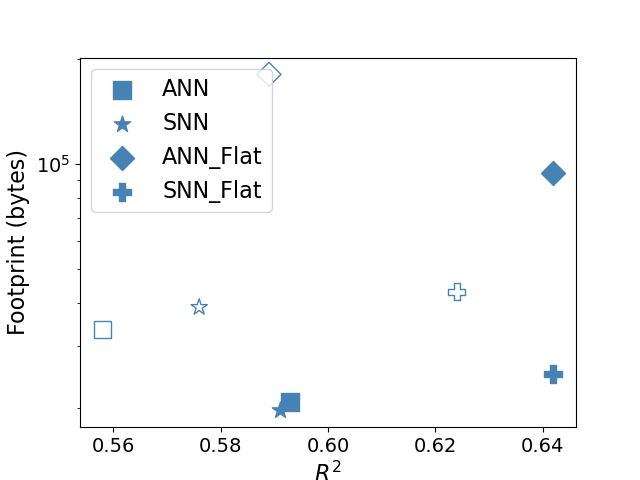
\includegraphics[width=1\linewidth]{figures/Memory_vs_Accuracy.png}
%  \caption{A subfigure}
  \label{fig:sub1}
\end{subfigure}%
\begin{subfigure}{0.5\textwidth}
  \centering
  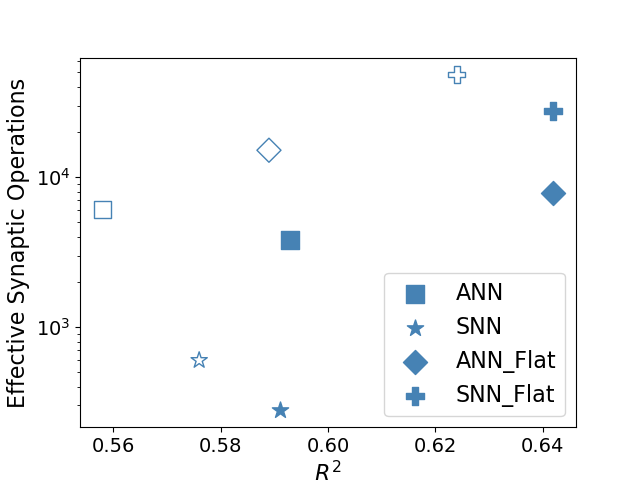
\includegraphics[width=1\linewidth]{figures/Computes_vs_Accuracy.png}
%\caption{A subfigure}
  \label{fig:sub2}
\end{subfigure}
\caption{Footprint and effective synaptic operations vs $R^2$, for four task baselines. Each model has two points: the solid marker represents NHP Indy, and the hollow marker represents NHP Loco.}
\label{fig:motor_result}
\end{figure}

We conduct further exploration for increasing task accuracies with more complex ANN and SNN models: ANN\_Flat and SNN\_Flat. For these networks, 50 data samples of buffered input are split into $n_p=7$ accumulated bins. For ANN\_Flat, the 7 bins are spatially flattened as input to the network, so its topology is ($7\times N_{ch}$)-32-48-2. 
SNN\_Flat uses the $N_{ch}$-32-48-2 topology, and the 7 bins are temporally flattened as input, presented to the network as separate input timesteps. Each prediction still uses the membrane potential of the output neurons after input timesteps, and the network is reset for each prediction. Layer normalization is also applied on the SNN\_Flat inputs.

Figure \ref{fig:motor_result} shows plots of complexity and predictive quality of all four baseline networks. Both flattened networks demonstrate significantly greater $R^2$ performance than the other two networks. However, the larger input dimension of the ANN\_Flat network is reflected in its greater footprint, and the increased model timesteps and layer normalization sharply increase the effective operations of SNN\_Flat by two orders of magnitude compared to the simpler SNN. Thus, while input flattening and normalization increase the quality of model predictions for ANNs and SNNs, each comes with a significant complexity trade-off. 
% Further research is motivated in computationally efficient model performance enhancement, such as weight plasticity or neuron models, that may be directly supported by neuromorphic hardware.



\subsubsection*{Chaotic Function Prediction}
% TODO: need to figure out how to cite and position in terms of existing benchmarking with MG: https://www.sciencedirect.com/science/article/pii/S2666827022000275
% \cite{shahi2022prediction}
% \begin{table}[ht]
% \centerline{
% \renewcommand{\arraystretch}{1.2}
% \begin{tabular}{|c|c|c|c|c|c|ccc|}
% \hline
% \multirow{2}{*}{Baseline} &
%   \multirow{2}{*}{sMAPE} &
%   \multirow{2}{*}{\begin{tabular}[c]{@{}c@{}}Footprint\\ (bytes)\end{tabular}} &
%   \multirow{2}{*}{\begin{tabular}[c]{@{}c@{}}Frequency\\ (Hz)\end{tabular}} &
%   \multirow{2}{*}{\begin{tabular}[c]{@{}c@{}}Connection\\ Sparsity\end{tabular}} &
%   \multirow{2}{*}{\begin{tabular}[c]{@{}c@{}}Activation\\ Sparsity\end{tabular}} &
%   \multicolumn{3}{c|}{SynOps} \\ \cline{7-9} 
%         &       &          &    &     &       & \multicolumn{1}{c|}{Dense}    & \multicolumn{1}{c|}{Eff\_MACs} & Eff\_ACs \\ \hline
% ESN & 14.79 & $2.81 \times 10^5$ & - & 0.876 & 0.0 & \multicolumn{1}{c|}{$3.52 \times 10^{4}$} & \multicolumn{1}{c|}{$4.37 \times 10^{3}$}  & 0 \\ \hline
% LSTM  & 13.37 & $4.90 \times 10^5$ & - & 0.0 & 0.530 & \multicolumn{1}{c|}{$6.03 \times 10^{4}$} & \multicolumn{1}{c|}{$6.03\times 10^{4}$}  & 0 \\ \hline
% \end{tabular}
% }
% \caption{Baseline results for the chaotic function prediction task. Frequency is not reported as the data is a synthetic time-series, with no real time correlation.}
%     \label{tab:MackeyGlass_resuls}
% \end{table}

\begin{table}[ht]
\centerline{
\renewcommand{\arraystretch}{1.3}
\begin{tabular}{c|cccccccc} \thickhline
\multirow{2}{*}{Baseline} &
  \multirow{2}{*}{\begin{tabular}[c]{@{}c@{}}sMAPE\end{tabular}} &
  \multirow{2}{*}{\begin{tabular}[c]{@{}c@{}}Footprint\\ (bytes)\end{tabular}} &
  \multirow{2}{*}{\begin{tabular}[c]{@{}c@{}}Model Exec.\\ Rate (Hz)\end{tabular}} &
  \multirow{2}{*}{\begin{tabular}[c]{@{}c@{}}Connection\\ Sparsity\end{tabular}} &
  \multirow{2}{*}{\begin{tabular}[c]{@{}c@{}}Activation\\ Sparsity\end{tabular}} &
  \multicolumn{3}{c}{SynOps (per model exec.)} \\ \cline{7-9} 
        &       &          &    &     &       & \multicolumn{1}{c}{Dense}    & \multicolumn{1}{c}{Eff\_MACs} & Eff\_ACs \\ \hline
ESN & 14.79 & $2.81 \times 10^5$ & - & 0.876 & 0.0 & \multicolumn{1}{c}{$3.52 \times 10^{4}$} & \multicolumn{1}{c}{$4.37 \times 10^{3}$}  & 0 \\ 
LSTM  & 13.37 & $4.90 \times 10^5$ & - & 0.0 & 0.530 & \multicolumn{1}{c}{$6.03 \times 10^{4}$} & \multicolumn{1}{c}{$6.03\times 10^{4}$}  & 0 \\ \thickhline
\end{tabular}
}
\caption{Baseline results for the chaotic function prediction task. Execution rate is not reported as the data is a synthetic time series, with no real-time correlation.}
    \label{tab:MackeyGlass_resuls}
\end{table}

The chaotic function prediction task has two recurrent ANN baselines, which feature distinct network architectures:

\begin{itemize}
        \item \textbf{Long short-term memory (LSTM)} -- LSTMs are a class of recurrent ANN architectures~\cite{Hochreiter1997}, utilizing multiple gates for selective retention or omission of past information. The LSTM baseline consists of a single LSTM with a hidden state of 100 neurons, followed by a feed-forward layer to produce single-dimension output predictions. 
        In addition, the LSTM baseline utilizes explicit memory by buffering 50 previous datapoints, spatially flattening them into 50 input channels.
        
        \item \textbf{Echo state network (ESN)} -- ESNs are randomized recurrent ANNs that belong to a class of algorithms known collectively as reservoir computing~\cite{ScardapaneRandomness2017}, featuring more biologically-inspired principles than LSTMs despite not being spiking networks. Standard ESNs have only one hidden layer (the reservoir), where synaptic connections projecting input data to the hidden layer and recurrent synaptic connections within the hidden layer are chosen randomly and stay fixed during the training. 
        % The only part of the network that is trained (referred to as the readout matrix) are the connections from the hidden and input layers to the output layer. 
        The model architecture for the ESN baseline has two neurons in the input layer, which projects the Mackey-Glass function input and additional constant bias input into a hidden layer of 186 neurons. Within the hidden layer, the probability of recurrent connections is set to 0.11. 
        % The training of the readout matrix was done using the standard teacher forcing procedure that, for the given time series, collected a matrix with activations of the input and hidden layers of the ESN and a vector with the corresponding ground truth values for the output layer.  This information was used to obtain the readout matrix with the regularized least squares estimator, Methods~\ref{sec:methods:algorithm:baselines}.
        
        
    
    \end{itemize}
The LSTM and ESN models were evaluated on a Mackey-Glass time series with $\tau=17$. The model is evaluated over 30 instantiations of the system; in each instance the start point is shifted forward by half of the Lyapunov time. The model is re-initialized and re-trained on each instance, and the results are averaged over all 30 instances. 

% JY: moved into methods
% The LSTM baseline shares characteristics with other baselines of a high effective-to-dense synaptic operation ratio, with a significant activation sparsity. Here, the internal sigmoid and $\tanh$ functions of the LSTM gates are not considered to be neuron activations, thus activations only account for the ReLU between the final LSTM cell and output layer. 

The ESN model is architecturally unique compared to the other ANN and SNN baselines. The connection sparsity metric ($0.876$) reflects the high number of zero-weight connections across its reservoir hidden layer. Due to this sparsity, hardware with support for sparse synaptic representation by ignoring zero weights would require less memory to represent the network, thus decreasing the deployed footprint of the model. The high connection sparsity of the ESN leads to significant reduction in synaptic operations - the ESN uses an order of magnitude fewer effective operations ($4.37\times10^3)$ than the LSTM ($6.03\times10^4$), while achieving comparable sMAPE. The activation sparsity of the ESN is 0 due to neurons using $\tanh(\cdot)$, rather than ReLU activations.



\begin{figure}[ht]
            \centering
            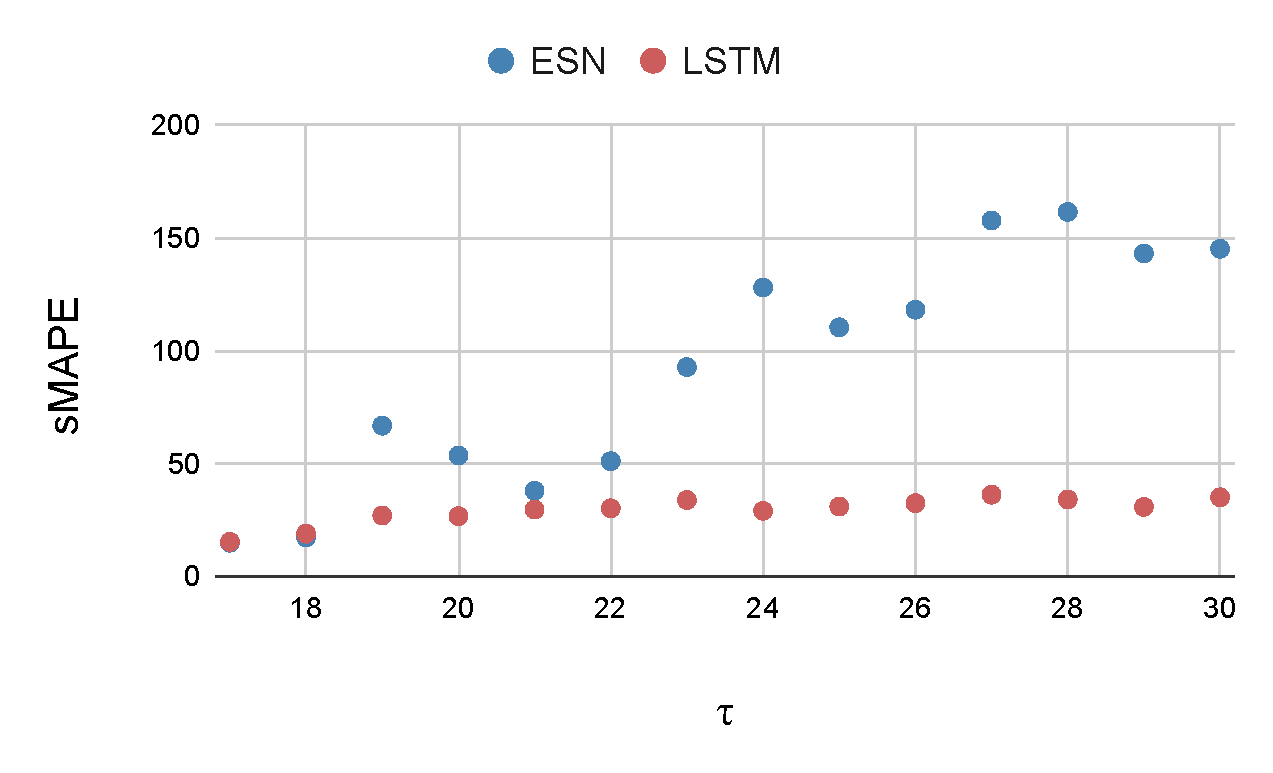
\includegraphics[width=.70\textwidth]{figures/mg_vary_tau.pdf}
            \caption{ESN and LSTM models evaluated on varying Mackey-Glass time series using a constant set of hyperparameters.}
        \label{fig:mackey_glass_function_performance}
    \end{figure}

Furthermore, we show the generalization and robustness capabilities of the particular ESN and LSTM models by applying them, with fixed hyperparameter sets, to other Mackey-Glass time series. Figure \ref{fig:mackey_glass_function_performance} shows the sMAPE score of the models over varied time series with the $\tau$ Mackey-Glass parameter varying between 17 and 30. The models were trained independently for each time series.
As the Mackey-Glass $\tau$ parameter characterizes the time-delay of the system, its increase roughly corresponds to prediction difficulty, shown by the increasing sMAPE trend through the plot. Notably, the LSTM maintains an error that is relatively lower than that of the ESN for all $\tau > 18$. However, the LSTM uses explicit memory via input buffering, so it is conjectured that the historical data allows for greater robustness to the varying time series characteristics. The ESN uses only one previous timestep, so its memory is only implicitly retained within its hidden layer. While the ESN tunes well to the $\tau$=17 case and demonstrates greatly reduced effective operations compared to the LSTM, the same set of hyperparameters does not generalize as well to other time series. Further research is motivated in explicit memory buffers versus implicit memory within the network state for trade-offs in single-series forecasting performance, complexity, and generalization capability.

\subsubsection*{Discussion and Opportunities for Further Research}
Baseline results for the four v1.0 algorithm track tasks compare the correctness and complexities of various solution types. Compared to ANNs, SNNs and ESNs demonstrate complexity advantages such as smaller footprints, high sparsity, and accumulate rather than multiply-and-accumulate operations. Especially on the motor prediction and chaotic function prediction regression tasks, the SNN and ESN baselines already achieve competitive correctness at lower complexity than the ANN and LSTM counterparts. Further research opportunities in model architectures, data pre-processing and buffering, and training paradigms to achieve greater performance is enabled by the standard framework and tooling provided by NeuroBench.
\section*{System Track Benchmark Framework}
% Target word count between 750 and 1000.

While the algorithm track aims to benchmark solutions in a system-independent manner via complexity analysis, the NeuroBench system track aims to evaluate deployed execution time, throughput, and efficiency of systems comprised of an algorithm deployed and tailored to a hardware platform. \secondrev{Previous benchmark studies have examined neuromorphic systems under various applications, including keyword spotting~\cite{blouw2019, bos2024micropowerspokenkeywordspotting}, audio and video processing~\cite{shrestha24efficient}, and combinatorial optimization~\cite{chen2024onoffneuromorphicisingmachines, pierro2024solvingquboloihi2}. While these studies have demonstrated neuromorphic system advantages, the benchmark tasks have been unaligned. In order for the hallmarks of neuromorphic hardware to be aptly judged against conventional systems and foster the expansion of neuromorphic solutions, transparent and objective comparisons must be made on standard tasks between sufficiently mature neuromorphic systems head-to-head, as well as against conventional systems.}

    \begin{figure}[ht]
            \centering
            
\includegraphics[width=.85\textwidth]{figures/system_types.png}
            \caption{Types of neuromorphic systems at various integration scales.}
        \label{fig:system_types}
    \end{figure}

A key challenge for benchmarking neuromorphic hardware is that systems are implemented and deployed at vastly different scales to serve diverse applications, from cloud services (e.g., multi-chip platforms like Loihi~\cite{Davies18loihi} and SpiNNaker~\cite{mayr2019spinnaker}) to embedded sensing intelligence (e.g., Speck~\cite{synsensespeck} and SNP~\cite{InnateraSNP, Levy2021}). This range is visualized in Figure~\ref{fig:system_types}. \secondrev{Existing benchmarks for conventional systems have individual focuses across high-performance~\cite{top500}, datacenter-level computing~\cite{Reddi2020}, and embedded processing~\cite{banbury2021mlperf}. 
Thus, rather than pursuing a one-size-fits-all suite of tasks, the goal of the NeuroBench system track is to develop benchmarks at various scales and use cases, under multiple application areas in which both conventional and neuromorphic platforms may compete. The selected v1.0 NeuroBench system track benchmarks represent key commercial application areas for existing systems, and they differ from the tasks in the algorithm track, which are more research-oriented. As benchmark results continue to identify properties of highly effective algorithms and systems, the two tracks will converge to the same selction of tasks that are seen as the most impactful for future progress in the field.}

\secondrev{In this section, we present the system track guidelines outlining metrics and tasks, representing collective design between multiple owners and vendors of neuromorphic hardware. Baseline benchmark results for neuromorphic and conventional systems are reported, and further official results will be collected and announced at a regular cadence, akin to the MLPerf suite~\cite{mlperf_policies}. As with all other facets of the NeuroBench framework, the system track guidelines will continue to be adapted and extended iteratively as benchmark results are produced and shared. Up-to-date information on the latest benchmarks and official results can be found on the NeuroBench website (\url{https://neurobench.ai/}).}

% As the system track benchmark tooling is currently under development, insight from the algorithm track's early results will be exploited towards a future release of the detailed harness documentation, benchmark procedure, and baselines for the system track by the end of 2024.

    \subsection*{System Track Metrics}
    \secondrev{In order to be representative of the properties of a deployed system, the system benchmarks, like the algorithm benchmarks, are assessed at the task level for the overall system, as opposed to operation- or kernel-level assessment of individual components. Task-level benchmarks enable straightforward comparison between systems of any type with regard to their abilities to solve problems, and the overall system-level measurement describes the realistic capability and efficiency of a whole solution.}

    \secondrev{Each individual system benchmark uses task-specific metrics aligned with \textit{correctness}, \textit{timing}, and \textit{efficiency} to measure the system under test (SUT). The following general considerations are applied to each category:}
    % % The following performance metrics describe what is considered a system-level evaluation. 
    % \sout{For ease of comparison and benchmark result analysis, key features of the NeuroBench system track are consistent with features from the widely-adopted machine learning  system benchmark MLPerf Inference~\cite{Reddi2020}.}

    % \TODO{Remove details about Task Scenarios, since it doesn't appear that the system benchmarks are consistent enough with the different scenarios. Make sure that the content serves the results report from Xylo.}

    % \paragraph{Task Scenarios.} Where applicable, the NeuroBench system track will utilize benchmark task scenarios from MLPerf. MLPerf describes task scenarios under which system benchmarks are presented to the system under test (SUT). For large-scale batched processing, MLPerf defines the \textbf{Offline} and \textbf{Server} scenarios, which are latency-unconstrained and latency-constrained, respectively, with performance measured in terms of prediction throughput. For batch-size-1 processing, MLPerf defines \textbf{Single-stream} scenarios, for which performance is measured in terms of prediction latency.

    % However, the MLPerf task scenarios all consider data as discrete samples, and therefore do not fit with some key neuromorphic system applications. The NeuroBench system track thus defines two additional task scenarios: \textbf{Real-time} and \textbf{Optimization}. \textit{Real-time} uses continuous data streams (e.g., from an event camera), which must be processed online by the SUT, in contrast with the \textit{Single-stream} scenario, where samples are sent only once the SUT has completed processing. Optimization applications use heuristic methods for otherwise intractable problems, and thus do not have notions of sample throughput or sample latency. The \textit{Optimization} scenario benchmarks will report latency for the SUT to reach multiple correctness thresholds, as many approaches find sucessively improved solutions over time.
    

    % For each task and scenario, the following metric categories are reported:
    \begin{itemize}
        \item \textbf{Correctness} -- \secondrev{In other system benchmarks, such as the closed category of the MLPerf Inference framework~\cite{Reddi2020}, the same trained model is used to benchmark all SUTs, and a correctness threshold is imposed to ensure optimizations such as lower precision do not disrupt task performance.}
        
        Due to the tight coupling between an algorithm and its system implementation in many existing neuromorphic hardware solutions, the particular model used to solve a NeuroBench system track benchmark task is unconstrained. Therefore, correctness must be measured to verify the validity of the solution. No correctness thresholds are imposed on submissions, but the benchmark leaderboard will impose tiers of solution correctness on submissions to evaluate accuracy-efficiency trade-offs of system approaches.
        
        \item \textbf{Timing} -- \secondrev{Depending on the task, timing performance can include measurements of sample throughput or execution time. Individually, the former entails an offline, batched inference benchmark, while the latter aligns with a streaming benchmark, in which one inference does not start until the previous one ends. Together, both throughput and execution time should be reported for tasks in which the SUT runs multiple inferences at any given time, each representing a request which must be responded to within a constrained window. The MLPerf Inference framework has defined widely-adopted general task scenarios corresponding to each of these categories (offline, single-stream, and server, respectively), and the NeuroBench system track will use these scenario guidelines where applicable to maintain consistency and build on conventional frameworks.}

        \secondrev{In addition, neuromorphic systems are also applied to tasks in which there is no notion of discrete sample throughput or execution, such as for heuristic approximations of intractable problems or operation over a continuous stream of data (e.g., from an event camera). Timing performance should be defined on a per-benchmark basis for such tasks, such as a time-to-solution latency or percentage of execution which exceeds a real-time threshold.}
        
        % Depending on the task scenario, the performance of the system is measured differently. The \textit{Offline} and \textit{Server} scenarios report throughput, while the \textit{Single-stream} scenario reports latency. The \textit{Real-time} scenario similarly reports latency, which for a large portion of execution (e.g., 90\%, defined per-benchmark) must not exceed a real-time threshold, or else the submission is not considered valid. The \textit{Optimization} scenario reports the time to solution at various solution quality thresholds, defined per-benchmark.
        
        \item \textbf{Efficiency} -- 
        Conventional system benchmarks such as TOP500~\cite{top500} for HPC and MLPerf Inference~\cite{Reddi2020} for deep learning do not require power measurement submission in the main benchmark, instead allowing for separate submissions to an adjacent power track (Green500~\cite{green500} and MLPerf Power~\cite{mlperfpower}, respectively). Not only has efficiency been usually considered as a second-order metric for conventional systems, it is also notoriously difficult to precisely measure. However, as energy efficiency is a key hallmark of biology and thus is a focus of neuromorphic research, power and energy consumption must be first-order metrics in the NeuroBench system track. \secondrev{Similarly to timing metrics, efficiency metrics should be tailored on a per-benchmark basis, i.e., a real-time always-on processing task may focus on average power, while offline batched systems focusing on high-throughput inference may focus on both peak power and energy per inference.}
        
        % The \textit{Server}, \textit{Offline}, and \textit{Real-time} scenarios report average power as their batched and online processing is continuous, the \textit{Single-stream} scenario reports the energy per-sample, and the \textit{Optimization} scenario reports total energy consumed at each solution quality threshold.
        
        % For tasks in the offline and server scenarios, average power is measured, while single-stream task scenarios intended for edge devices measure average energy consumption per sample. Further information about the power measurements is provided in the Methods section.
        
    \end{itemize}

    \secondrev{As neuromorphic systems currently explore a broad range of varied implementation approaches, board-level integration, and developmental stages of hardware, platform diversity poses difficult challenges for completely consistent hardware measurement methodologies (e.g., consistent power meters, chip interfaces, and data loading). Thus, to enable an initial step towards consistency in the system track while ensuring openness, we focus on the development of guidelines for transparent documentation, as they provide the foundation for shared methodology among highly diverse solutions. While there may be differences in how metrics are measured, salient details will be available to contextualize the results, allowing for holistic analysis, and leading the way for future consistency by enforcing transparency.}

    Benchmark submissions may perform separate runs to report performance and power in order to demonstrate system flexibility (e.g., a `performance-mode' run optimal for execution time and an `efficiency-mode' run optimal for energy), however in all runs, both metrics must be reported.

    Importantly for the NeuroBench system track, in measuring timing and efficiency, data pre- and post-processing must be taken into account. Neuromorphic methods will often consume and produce non-standard (e.g., event-based) data modalities, the processing of which may consume a significant amount of the overall execution time and may not be computed on the neuromorphic hardware itself. As many instances of neuromorphic hardware cannot be deployed without such associated processing, it is essential that measurements capture the cost of data processing, which stands in contrast with conventional system benchmarks whose measurements start from pre-processed data~\cite{mlperf_policies}.

    % \revision{Correctness and performance metrics are relatively straightforward to implement consistently across systems, and specific rules and measurement guidelines from MLPerf Inference~\cite{Reddi2020} will be used where applicable, with benchmark-specific modifications. However, due to the highly varied implementation approaches, board-level integration, and developmental stages of neuromorphic hardware, a first step towards 

    % \revision{Neuromorphic hardware may be implemented as a standalone system which covers the whole processing pipeline from raw data to prediction. However, the hardware may also be integrated as an accelerator unit which relies on a host CPU for pre-/post-processing. For standalone systems, performance and efficiency measurements must be monitored at the full-chip level. For accelerator systems, all processing from host integration must be included in the measurements, however the aggregated results should be broken into the host and neuromorphic components so that the full system can be characterized. Detailed hardware measurement guidelines are included in the Methods section.} \TODO{Check here}

    % \TODO{Integrate the following text:}

    % \revision{Where applicable, rules and measurement guidelines from MLPerf Inference~\cite{Reddi2020} will be used. Accuracy and performance (latency or throughput) can be measured in accordance with these rules and as noted further by the individual benchmarks.}

    % \revision{However, due to the highly varied implementation features, board integration, and developmental progress of neuromorphic hardware, an initial benchmark framework cannot expect fully consistent power measurement across all systems. Thus, power measurement is instead standardized under a common transparent documentation structure, such that while results may not be directly comparable, there is still the ability to holistically analyze results and move towards future consistency.}
    
    % \revision{The NeuroBench power specification highlights component-level granularity and inclusion of all pre-/post-processing hardware. 
    % Any on-board components which contribute to workload calculation should be included.} \TODO{List further notes about power spec or where it will be defined. Or maybe don't include further detail and instead move the prior paragraph up into the main text? It is an important idea.}

    \subsection*{System Track Benchmarks}
    \secondrev{Two benchmark specifications for the v1.0 system track are defined in this article, covering embedded to datacenter scales. Full benchmark details are available in the Methods section.}
    \begin{itemize}
        \item \textbf{Acoustic Scene Classification} -- The acoustic scene classification benchmark challenges systems to classify audio into predefined categories based on the environmental audio context. 
        % Utilising such an application as a vehicle for benchmarking is beneficial from varied perspectives. Real-world applicability of the use case can relatively easily be seen within, for example, hearables to adjust sound equalisation profile, to more appropriately target microphone noise cancellation or to support active noise cancellation. 
        Such capabilities are key for hearable devices, which can utilize them to automatically adjust sound equalisation profiles, appropriately target microphone denoising, and support active noise cancellation.
        The application further challenges systems to fulfill technical requirements, such as always-on and real-time operation, and time series processing.
        Acoustic scenes provide a rich repertoire of features that are necessary for prediction, thus this task is a complement to keyword classification, which mainly focuses on shorter-term features (e.g., phonemes) with a relatively smaller feature repertoire.
        % Furthermore, the chosen dataset and application would impart a requirement on the model and system to process and interpret a wide and rich repertoire of features in order to correctly produce a prediction. This task could complement that of keyword spotting which mainly focuses on shorter-term features (for example, phonemes) that are part of a relatively smaller repertoire.  

        % Leveraging the datasets from the DCASE~\cite{Heittola2020} challenge, we establish an acoustic scene classification benchmark that would evaluate the classification capabilities of both neuromorphic systems and conventional computing platforms. 
        
        The benchmark evaluates the classification capabilities of both neuromorphic systems and conventional computing platforms using \revision{datasets from the DCASE challenge~\cite{Heittola2020}.} 
        %(if permissible, subject to license).
        These datasets consist of a myriad of audio recordings from diverse environments, including airports, public parks, and buses, thus providing a comprehensive foundation for testing both application- and system-level performance. \secondrev{The NeuroBench subset of the DCASE dataset includes 41360/16240 train/test samples across four classes (airport, street traffic, bus, park).}
        % While the goal of an application-level task could be to also assess the generalisation performance, as stated as goal within the DCASE challenge itself, the system track would not necessarily enforce such stringent accuracy targets.

        % JY: attempted to fit this task into the Real-time task scenario, as it would be most coherent to provide specs for both the Real-time and Optimization new task scenarios.
        \secondrev{The task will be presented under the single-stream task scenario, providing one 1-second sample to the SUT at a time. Classification probability will be sampled to determine the correctness of the prediction. As the NeuroBench system track allows for unconstrained algorithmic implementation, pre-processing and inference metrics should be separately measured and reported together, which differs from prior system benchmarking that only measure inference~\cite{blouw2019, banbury2021mlperf}. 
        Timing results report on-device average execution time per sample.
        Since the platform diversity of edge-targeted systems poses inherent inconsistencies in efficiency measurement, power should be reported under idle and active contexts, following prior benchmark study methodology~\cite{blouw2019}. Idle power measures the system prepared for inference with the model loaded, and active power measures the system running pre-processing or inference. The difference between active and idle measurements offers dynamic power, which is used along with execution time to calculate dynamic energy-per-sample.}
        % The average power measured during inference is a key indicator of the efficiency and always-on capability of the SUT, and inference latency will be measured in terms of the prediction time relative to the onset of each new acoustic scene.
        
        % The metrics produced within this system track benchmark are: average power per inference, accuracy across a validation dataset, average inference latency. As in the case of the QUBO task and depending on the chosen solution, the impact of inference duration may be traded off to evaluate accuracy or energy scaling. In opposition to the QUBO task, the scale of the problem cannot be arbitrarily varied, therefore there exists the possibility that certain systems may be over or under-sized, and therefore power or accuracy may be scaled proportionally. The task would be profiled mainly in a single-stream fashion, wherein individual 1 second samples are used to report the above KPIs. The samples could also be stitched together to emulate a real-time scenario, however this may impose a restriction on the number and type of devices that can participate in the benchmark as storing many second samples may be outside of the ability of certain systems. 

        

        \item \textbf{QUBO} -- % Neuromorphic systems have repeatedly excelled in mathematic optimization heuristics. These tasks optimize a cost function by iterative updates of a large range of variables, operations that benefit from the tight compute-memory integration and massive parallelism of neuromorphic processors \cite{Aimone2022}. 
        As a non-ML task, NeuroBench incorporates quadratic unconstrained binary optimization (QUBO). QUBO is a particularly beneficial first optimization task for NeuroBench for two reasons. First, the binary variables are a natural fit for neuromorphic systems with purely binary spike communication. Second, real-world QUBO applications typically feature sparse cost matrices~\cite{koch2022} which benefit from the sparse synaptic connectivity and execution that neuromorphic systems are often optimized for \cite{Aimone2022}. The initial set of QUBO workloads in NeuroBench searches for the maximum independent (i.e. unconnected) set of nodes in graphs, a task that has wide applications across industry and academia, such as resource allocation in wireless networks, portfolio optimization, and task scheduling~\cite{wurtz2024industryapplicationsneutralatomquantum}.
        % Correctness of the task is the largest independent set found by the SUT, and it is compared in relation to the best result known for a particular dataset.
        
        NeuroBench provides a QUBO generator that can uniquely specify each workload by three specific parameters provided by the benchmark: the number of graph nodes, the density of graph connections, and a random seed. The generator provides a large dataset for reliable statistics and allows scaling from modest workloads for small-scale and prototype systems to large workloads for larger-scale systems. \secondrev{The graph sizes specified by the benchmark increase in a pseudo-geometric progression (10, 25, 50, 100, 250, ...), and submissions are encouraged to extend the problem size to the limits of the SUT. Graph density ranges from 1\% to 30\%, in order to show the relationship between the number of connections and SUT power. 5 random seeds for each setting should be tested.}
        % As an \textit{Optimization} scenario task, the time-to-solution latency aggregated energy consumption at various correctness thresholds is measured. In addition, the maximum supported workload size is reported.
        % The SUT is evaluated based on three metrics: The first success metric is the maximum supported workload size. The second and third metric is the time and energy required to obtain pre-defined levels of optimality, respectively. The solution optimality is measured by the size of the independent set of nodes found by the SUT.

        % The SUT is evaluated based on three metrics: The first success metric is the maximum supported workload size. The second and third metric is the timing and energy efficiency of the system, respectively. For optimization algorithms, these metrics can be measured in either of two ways: The first version of NeuroBench will measure the solution optimality and energy consumption reached during a pre-set runtime. The second version of NeuroBench will add a benchmarking routine that defines a target solution optimality and determines the time and energy required to achieve it, which will be released once reasonable target solution optimality have been determined using runs of conventional reference solvers. The solution optimality is measured by the cost of the QUBO cost function for the variable assignment obtained by the SUT.

        \secondrev{Optimization algorithms use heuristic methods to iteratively refine approximate solutions to intractable problems that cannot be completely solved. The QUBO benchmark thus measures solution optimality and energy consumption after fixed, pre-set runtimes, removing any timing measurement. Solution optimality is defined as BKS-Gap, a relative gap between the current SUT's solution compared against the best-known solution (BKS) to the same problem found using a high-powered solver with a long runtime.
        % Thus, the QUBO task is presented under two scenarios. The first is to measure solution optimality and energy consumption after fixed, pre-set runtimes, removing any timing meaesurement. The second is to define thresholds of solution optimality for given problems, and measure the latency and energy required for the SUT to reach each threshold. Solution optimality is defined as BKS-Gap\%, a relative gap between the current SUT's solution compared against the best-known solution (BKS) to the same problem found using a high-powered solver with a long runtime. Both scenarios are representative of optimization applications, so NeuroBench defines specifications for each. In this article, baselines for the former scenario are reported.
        }
        
        % \secondrev{In addition to timing and efficiency measurements under the two QUBO scenarios, when comparing neuromorphic systems head-to-head, each SUT should report the maximum supported workload size. While this may not be as important for von Neumann architecture systems with expandable working memory, neuromorphic systems often have co-located memory with processing, thus the metric highlights the scale of the SUT.}

        % JY: Commenting out these details for this paper
        % A community-wide benchmark must use protocols that support all hardware vendors. 
        % The first QUBO benchmark adopts QUBO problems where the Q-matrix can be represented by weights of at most 8-bit precision, aligned with the precision of synaptic weights in baseline neuromorphic systems. 
        % The Maximum Independent Set, for instance, requires both positive and negative weights but can be accommodated by eight bit precision. These values encode the presence or absence of an edge between two graph vertices. 
        % With increasing iterations, NeuroBench will also provide QUBO workloads that require greater weight precision to accompany and push the advancement of neuromorphic systems.
    
    \end{itemize}

% \subsection*{System Track Harness}
% \begin{figure}[ht]
%     \centering
%     \includesvg[width=.95\textwidth]{figures/alg_system_harness.svg}
%     \caption{\revision{An overview of the NeuroBench harness with support of the system track. The implementations of the system track components shown in blue are currently specific to the hardware backend, and common interfaces within the runtime allow that the harness can be modularly extended to various system backends.}}
%     \label{fig:alg_system_harness}
% \end{figure}

% \TODO{Considering again removing the system track harness figure, there are only shared data / task files and specifications in a repo. We can instead position the harness as a platform for which different systems can open-source their benchmarking scripts.}

% A diagram of the NeuroBench harness with extended support for the system track is shown in Figure~\ref{fig:alg_system_harness}. Blue boxes in the figure denote hardware-specific infrastructure components which will connect to the general top-level harness interfaces.

% \revision{Software toolchains such as Lava~\cite{lava}, Fugu~\cite{aimone2019composing}, NIR~\cite{NIR2023}, SPyNNaker~\cite{spynnaker}, Samna~\cite{samna}, among others, have been developed to interface with specific hardware platforms. Many of the stacks are built with general paradigms to support extension to any backend, and the community is actively moving towards developing standards for deployment tools.}

% \revision{In order to facilitate systematic hardware benchmarking in the present and further extensions in the future, the NeuroBench harness provides common interfaces within the runtime to allow modular execution for various backends. Initially, these components will be implemented using hardware-specific tools to optimize system benchmark performance. As standards mature, common tools such as model description frameworks and intermediate representations (IR) can be incorporated, reducing implementation complexity for benchmark users to test on many different platforms.}

% The side-by-side harness runtimes for the algorithm track and system track benchmarks provides users with a single tool for both types of analysis. As the algorithm and system tracks mature to support the same tasks, the harness will accelerate benchmarking by facilitating quick prototype complexity analysis followed by deployed performance measurement with minimal implementation overhead.

\subsection*{Baseline Results}

\secondrev{Baseline results for each of the two system track benchmarks are provided for a mature neuromorphic system against a conventional platform. Like for the algorithm track baseline results, the system track baselines are intended to snapshot the solution space and provide starting points for the task leaderboards. Further details on each baseline system are available in the Methods section, and in-depth system documentation for the Xylo ASC baseline and CPU/Loihi 2 QUBO baselines are provided by Ke et al.~\cite{ke2024neurobenchdcase2020acoustic} and Pierro et al.~\cite{pierro2024solvingquboloihi2}, respectively.}

\subsubsection*{Acoustic Scene Classification}


\secondrev{For the acoustic scene classification task, two baseline embedded systems are reported:
\begin{itemize}
    \item \textbf{CPU} -- The CPU baseline is an Arduino Nano 33 BLE, which uses an ARM Cortex M4 microcontroller for both pre-processing and inference. The digital audio sample is pre-processed using Mel-filterbank energies (MFE), and inference uses a conventional CNN. Execution time is measured using on-chip timers, and power is measured using total system power.
    \item \textbf{Xylo} -- The Synsense Xylo~\cite{synsensexylo} neuromorphic baseline uses a feed-forward SNN with multiple synaptic time constants~\cite{bos2024micropowerspokenkeywordspotting}. As the system is intended for continuous, real-time audio processing, the board uses an analog front end to pre-process analog audio signals directly from a microphone into spikes for the digital inference engine. To conform with a digital benchmark dataset, a simulator of the analog pre-processor generates spikes, which are routed to the inference module. Execution time and power are measured using on-board instruments.
\end{itemize}}

\begin{table}[ht]
\centerline{
\renewcommand{\arraystretch}{1.3}
% \begin{tabular}{@{}c|ccccccc@{}}
% \begin{tabular}{@{}c|cccccc@{}}
% \thickhline
% \multirow{2}{*}{Baseline} &
%   \multirow{2}{*}{Accuracy} &
%   \multirow{2}{*}{\begin{tabular}[c]{@{}c@{}}Latency\\ (ms)\end{tabular}} &
%   \multirow{2}{*}{\begin{tabular}[c]{@{}c@{}}Idle \\ Power (mW)\end{tabular}} &
%   \multirow{2}{*}{\begin{tabular}[c]{@{}c@{}}Active\\ Power (mW)\end{tabular}} &
%   \multirow{2}{*}{\begin{tabular}[c]{@{}c@{}}Dynamic \\ Power (mW)\end{tabular}} &
%   % \multirow{2}{*}{\begin{tabular}[c]{@{}c@{}}Active\\ Energy (mJ/inf)\end{tabular}} &
%   \multirow{2}{*}{\begin{tabular}[c]{@{}c@{}}Dynamic\\ Energy (mJ/inf)\end{tabular}} \\
%                       &                          &     &       &        &       &        &        \\ \hline
%           CPU         & \multirow{2}{*}{79.64\%} & 43  & 79.40 & 100.72 & 21.32 &  4.33  & 0.917   \\
%     (\textit{system-wise}) &                     & 45  & 79.40 & 100.15 & 20.75 &  4.51  & 0.934   \\ \hline
% Xylo & \multirow{2}{*}{76.00\%} & \textbf{N/A} & \textbf{N/A}   & 0.015  & \textbf{N/A}   & \textbf{N/A}    & \textbf{N/A}    \\
%  (\textit{component-wise})&                      & 40  & 0.298 & 0.503  & 0.205 & 0.0201 & 0.0082 \\ \thickhline
% \end{tabular}
%%%%%%%%%%%%%%%%%%% JY: The below block is the updated numbers / format
\begin{tabular}{@{}cc|cccccc@{}}
\toprule
\multicolumn{2}{c|}{\multirow{2}{*}{Baseline}}                        & \multirow{2}{*}{Accuracy} & \multirow{2}{*}{\begin{tabular}[c]{@{}c@{}}Execution\\ Time (ms)\end{tabular}} & \multirow{2}{*}{\begin{tabular}[c]{@{}c@{}}Idle \\ Power (mW)\end{tabular}} & \multirow{2}{*}{\begin{tabular}[c]{@{}c@{}}Active\\ Power (mW)\end{tabular}} & \multirow{2}{*}{\begin{tabular}[c]{@{}c@{}}Dynamic \\ Power (mW)\end{tabular}} & \multirow{2}{*}{\begin{tabular}[c]{@{}c@{}}Dynamic\\ Energy (mJ/inf)\end{tabular}} \\
\multicolumn{2}{c|}{}                                                 &                           &                                                                         &                                                                             &                                                                              &                                                                                &                                                                                    \\ \midrule
\multicolumn{1}{c|}{CPU}                       & \textit{pre-process} & \multirow{2}{*}{79.64\%}  & 43                                                                      & 79.40                                                                       & 100.72                                                                       & 21.32                                                                          & 0.917                                                                              \\
\multicolumn{1}{c|}{\textit{(system-wise)}}    & \textit{inference}   &                           & 45                                                                      & 79.40                                                                       & 100.15                                                                       & 20.75                                                                          & 0.934                                                                              \\ \midrule
\multicolumn{1}{c|}{Xylo}                      & \textit{pre-process*} & \multirow{2}{*}{79.90\%}  & -                                                                       & 0.00017*                                                             & 0.015*                                                                        & 0.015*                                                               & 0.015*                                                                                  \\
\multicolumn{1}{c|}{\textit{(component-wise)}} & \textit{inference}   &                           & 84                                                                      & 0.351                                                                       & 0.692                                                                        & 0.341                                                                          & 0.028                                                                             \\ \bottomrule
\end{tabular}
}
\caption{\secondrev{Baseline results for the acoustic scene classification task. Pre-processing of the Xylo (marked with an asterisk *) measures power of the analog pre-processor in real-time relative to the audio data, whereas other measurements are of digital components processing digital data on-hand. Idle Xylo pre-processing measures silence and active measures test data audio played to the device, and energy is measured over the sample duration of 1 second. CPU power is measured over the full Arduino system, as it does not have on-board power instrumentation, while Xylo power measures power consumed by the Xylo Audio 2 ASIC only. Dynamic power and energy provide proper comparison between the systems, and idle and active measurements are provided for transparency.}}
\label{tab:asc_results}
\end{table}



\secondrev{Table~\ref{tab:asc_results} lists baseline results for the neuromorphic Xylo system against an Arduino system. Compared to prior neuromorphic audio system benchmarking~\cite{blouw2019}, which takes a server-class CPU as a point of comparison, we adopt a fairer approach by focusing on low-power edge application and comparing against an Arduino embedded microprocessor. At comparable inference accuracy, Xylo exhibits $60.9\times$ less dynamic inference power and $33.4\times$ less dynamic inference energy consumption than the Arduino.
%Full details about the Xylo SNN, training, and measurement methodology are avaiable in Ke et al.~\cite{ke2024neurobenchdcase2020acoustic}
%Though this platform serves as a suitable comparison against the Xylo, the Arduino does not include any power instruments on-board or on-chip, and thus full system power must be measured externally. Meanwhile, the Xylo measures from on-board current instruments. The inconsistency is addressed by separating dynamic power as the difference between idle and active power measurements, though all are reported for transparency.
}

% \secondrev{The Edge Impulse platform~\cite{hymel2023edgeimpulsemlopsplatform} used to deploy the CPU baseline consists of commercially-developed tinyML optimizers and libraries for microcontroller devices such as the Arduino. At comparable inference accuracy, Xylo exhibits $60.9\times$ less dynamic inference power and $33.4\times$ less dynamic inference energy consumption than the Xylo. Full details about the Xylo SNN, training, and measurement methodology are avaiable in Ke et al.~\cite{ke2024neurobenchdcase2020acoustic}}

\subsubsection*{QUBO}
% \begin{table}[ht]
\centerline{
\renewcommand{\arraystretch}{1.5}
\begin{tabular}{c|cc}
\thickhline
\multirow{2}{*}{Baseline} &
  \multirow{2}{*}{\begin{tabular}[c]{@{}c@{}}Avg.\\ BKS-Gap \%\end{tabular}} &
  \multirow{2}{*}{\begin{tabular}[c]{@{}c@{}}Avg. Runtime \\ Power (W)\end{tabular}} \\
           &      &       \\ \hline
CPU - SA   & TODO & 87.78 \\ \hline
CPU - TABU & TODO & 97.56 \\ \hline
Loihi 2    & TODO & 2.62  \\ \thickhline
\end{tabular}
}
\caption{\secondrev{Baseline results for the QUBO task. Avg. BKS-Gap\% measures the average gap percentage between the solution found by the SUT and the best-known solution, averaged across fixed timeouts from $10^{-3}$ to $10^{2}$ seconds, graph sizes of $10^1$ to $10^3$, and graph density of 15\%. Average runtime power is measured over graph sizes of $10^1$ to $10^3$, and densities of 5\%, 15\%, and 30\%. Figures~\ref{fig:qubo_bksgap} and~\ref{fig:qubo_power} provide the breakdown of these results.} \TODO{Doesn't make sense to have a table since graph size changes things a log, and power increases as a function of graph size. Intel also prefer to keep the credit for their results, which means this benchmark will appear to be a copy.}}
\label{tab:qubo_results}
\end{table}
 
% \JY{TODO: The latest from Intel is that that they have lost the results for producing the figures, and would not prefer to spend the time to re-generate all of them. So all we have are the figures from their paper and a few numbers. Removed table.}

\begin{figure}[t]
    \centering
    \begin{subfigure}{0.48\textwidth}
        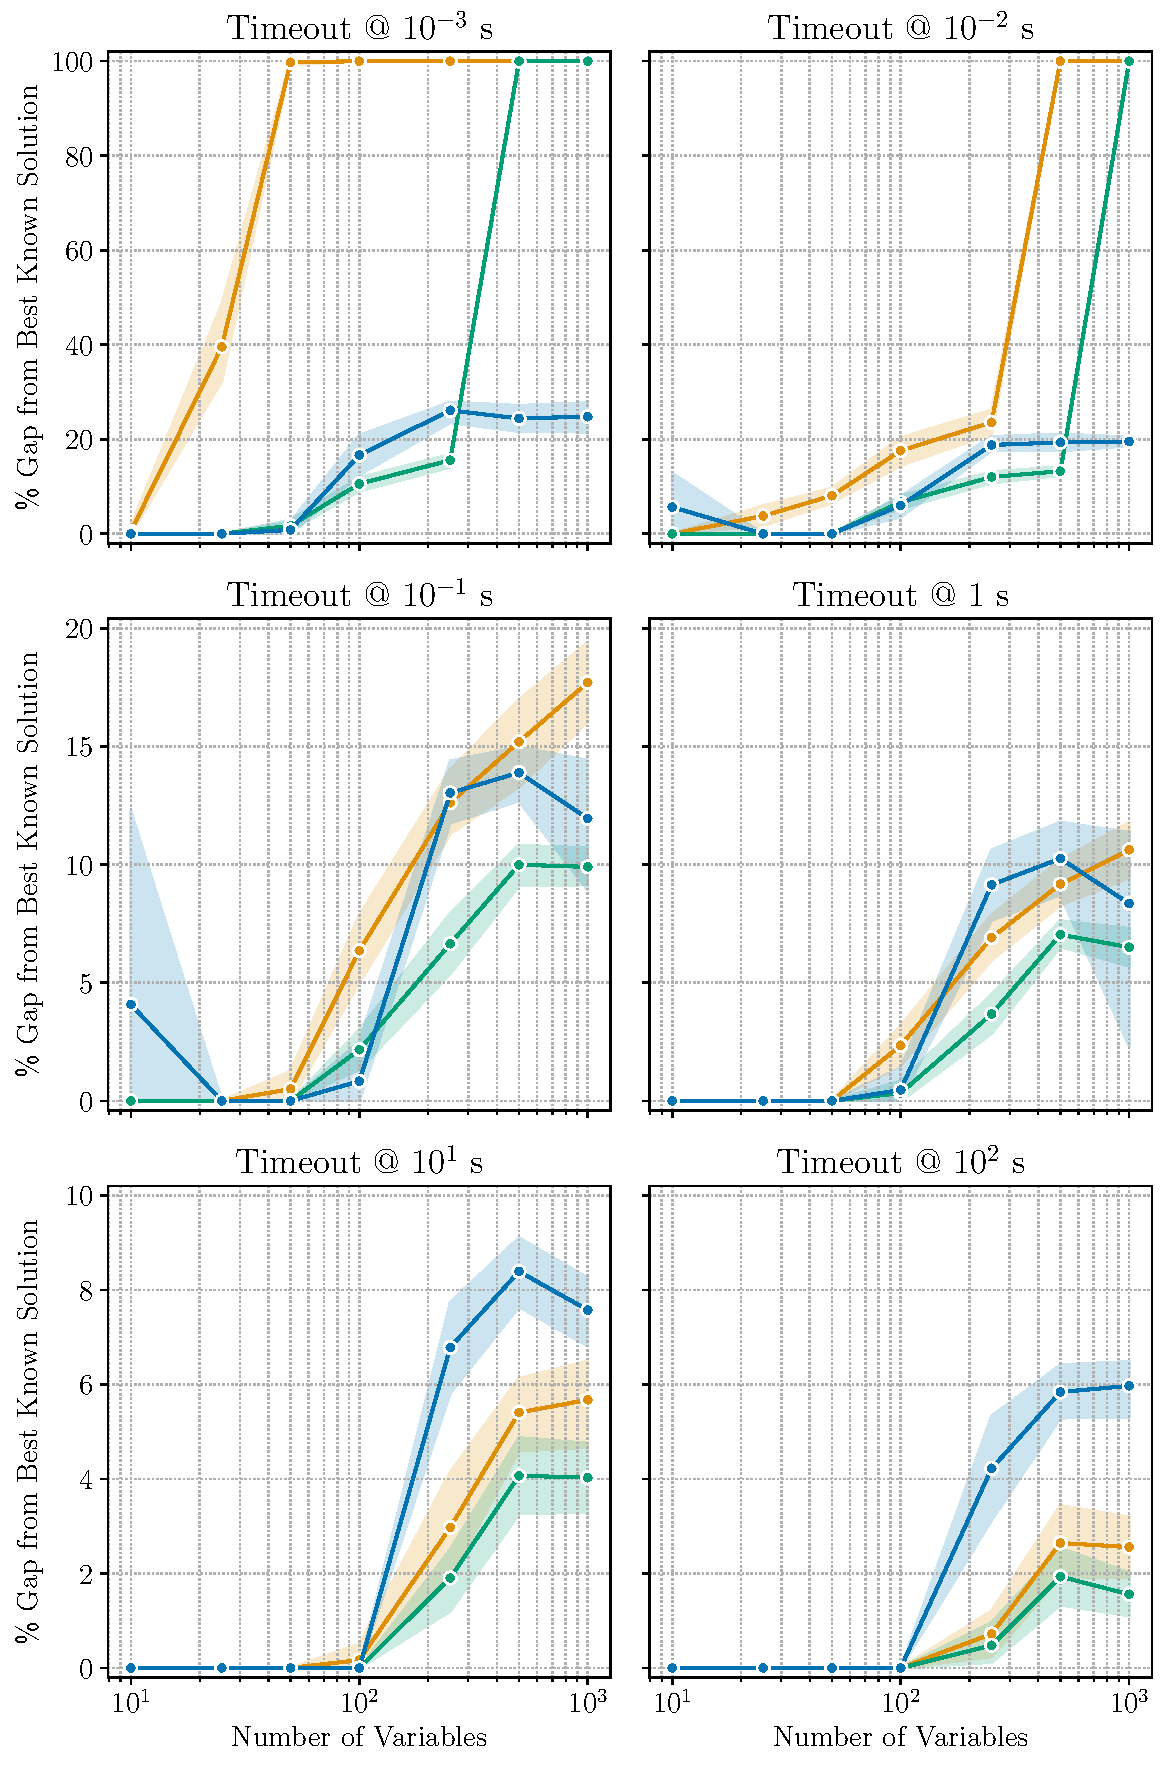
\includegraphics[width=\linewidth]{figures/mis_optimality_0.15.pdf}
    \vspace*{0.2cm}
    \end{subfigure}\\
    \begin{subfigure}{0.3\textwidth}
        
\includegraphics[width=\linewidth]{figures/legend.pdf}
    \end{subfigure}
    \caption{\secondrev{Percentage gap from the best known solution (BKS-Gap\%) for the QUBO workloads with QUBO matrices at $15\%$ density (lower is better). Results are shown for different timeouts of the QUBO solvers. Figure taken, with permission, from Pierro et al.~\cite{pierro2024solvingquboloihi2}.}}
    \label{fig:qubo_bksgap}
\end{figure}

\begin{figure}[t]
    \centering
        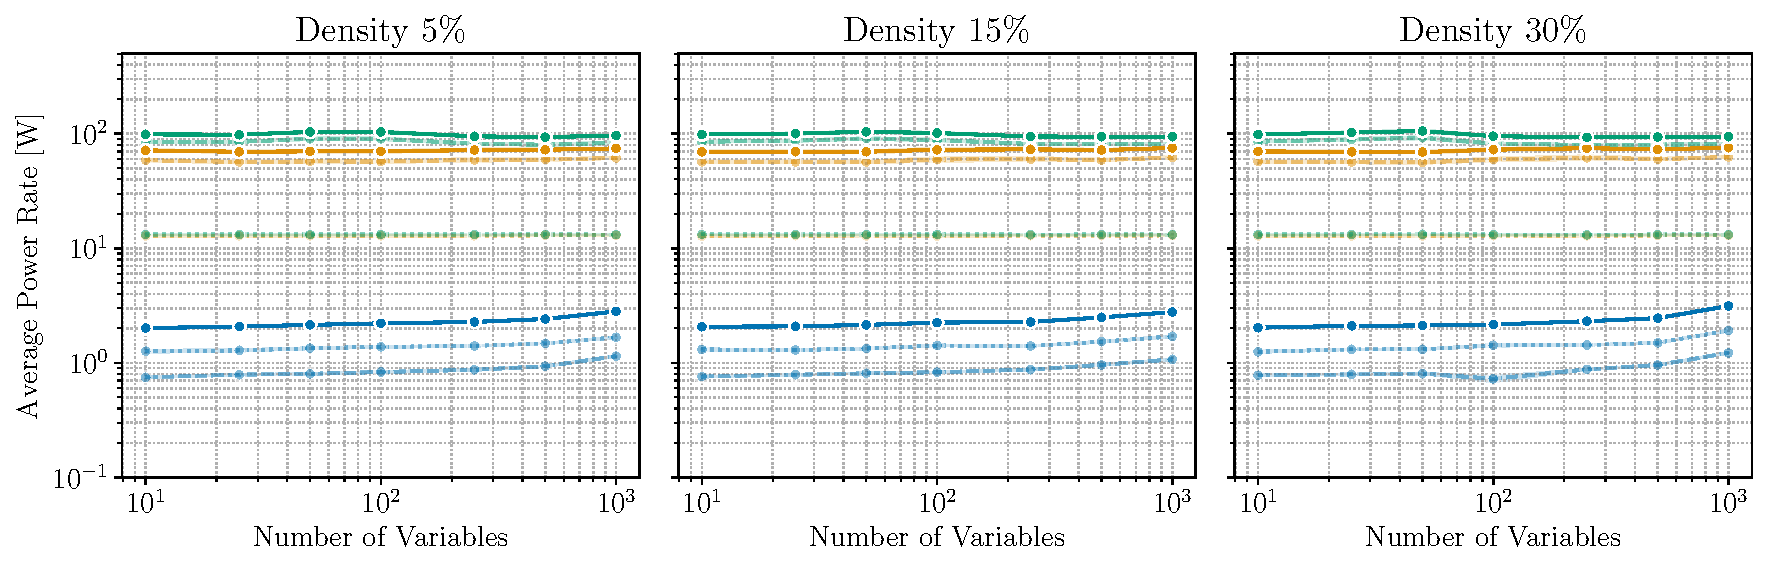
\includegraphics[width=\linewidth]{figures/mis_power.pdf}
    \vspace*{0.5cm}

\includegraphics[width=0.3\linewidth]{figures/legend.pdf}
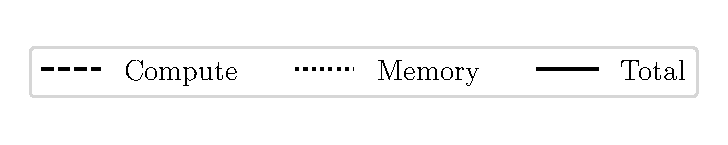
\includegraphics[width=0.35\linewidth]{figures/line_style_legend.pdf}
        \caption{\secondrev{Power consumption of the QUBO solvers running simulated annealing (SA) or TABU search on CPU, and the parallelized version of simulated annealing on Loihi 2. The CPU solvers require up to $37\times$ more power than the neuromorphic algorithm on Loihi 2. Since the QUBO workloads were run for a fixed timeout, differences in power consumption are equivalent to differences in energy consumption of the processors. Figure taken, with permission, from Pierro et al.~\cite{pierro2024solvingquboloihi2}.}}
        \label{fig:qubo_power}
\end{figure}

\secondrev{Three baselines are measured for the QUBO benchmark:
\begin{itemize}
    \item \textbf{Simulated Annealing (SA)} -- The simulated annealing solver uses Markov chain Monte Carlo (MCMC) sampling to probabilistically explore the search space. 
    \item \textbf{Tabu Search (TABU)} -- Tabu search solvers maintain and iterate a list of prohibited actions in order to prevent the search from remaining in local minima or revisiting states. Both the TABU and SA solver baselines use the D-Wave Samplers library~\cite{dwavesamplers} on an Intel Core i9-7920X desktop-class CPU, with power measured using Intel SoC Watch.
    \item \textbf{Loihi 2} -- The Loihi 2 neuromorphic system solver uses an SNN formulation of the simulated annealing algorithm which enables solving via neural dynamics, and parallelization via stochastic refractory periods. The baseline is implemented on one Loihi 2 chip on the 8-chip Kapoho Point board, and internal power instrumentation measures all compute and memory components of the chip.
\end{itemize}}

\secondrev{Figure~\ref{fig:qubo_bksgap} shows the optimality reached by the CPU- and Loihi 2-based solvers after different timeouts. For tight time constraints, at $10^{-2}$ seconds timeout or less, Loihi 2 finds feasible solutions to workloads $4\times$ larger than the CPU. But for timeout lasting $10$ seconds or longer, the CPU running TABU provides the lowest BKS-Gap, incentivizing algorithmic advances for neuromorphic optimization systems.}
\secondrev{Figure~\ref{fig:qubo_power} illustrates the power consumed during runtime. Across the workloads, the Loihi 2 solver requires $37.24\times$ less power compared to the best CPU solver.  
%All details on the solvers, benchmarking routine, and results have been provided by Pierro et al.~\cite{pierro2024solvingquboloihi2}.
}

\subsubsection*{Discussion and Future Work}
\secondrev{The initial baselines for the v1.0 system track compare correctness, timing, and efficiency of neuromorphic systems against conventional CPU systems in domains of both audio classification and optimization. Against mature, commercially-developed CPU systems, for both edge and server use cases, the neuromorphic systems show strong advantages in general efficiency, as well as further promises in terms of timing and correctness. 
%The benchmarks utilize collaboratively-defined task and methodology specifications, setting the groundwork for head-to-head neuromorphic system comparisons that will identify neuromorphic strengths and push towards standardization and development of better neuromorphic systems.
}

\secondrev{In future NeuroBench iterations, the system track benchmarks can be unified under common tooling, similar to the algorithm track. Software toolchains such as Lava~\cite{lava}, Fugu~\cite{aimone2019composing}, SPyNNaker~\cite{spynnaker}, and Samna~\cite{samna}, among others, have been developed to interface with specific hardware platforms. Many of the stacks are built with general paradigms to support extension to any backend, and the community is actively moving towards developing standards for deployment tools. The current v1.0 benchmark specifications allow for open algorithm and software design in order to demonstrate fully optimized performance for neuromorphic systems. As standards mature in the future, a core focus of the NeuroBench system track is to introduce a closed-algorithm benchmarking category that leverages the recently proposed NIR model description framework~\cite{NIR2024} as a general, cross-platform tool for benchmarking key workloads of interest across many different platforms.}
% Discussion section: succinct and no subheadings

\section*{Discussion} % 500-750 words maximum

% high level recap
Benchmarking neuromorphic computing has faced challenges stemming from the diversity of neuromorphic approaches, the range of implementation and deployment tools, and rapid research evolution.
NeuroBench addresses these challenges as a framework for the inclusive, actionable, and iterative benchmarking of neuromorphic solutions, by including novel tasks and metrics, open-source and extendable harness tooling, and facilitating systematic growth via community collaboration. NeuroBench is supported and developed by a broad community of neuromorphic researchers to be a standard, agreed-upon benchmarking framework for neuromorphic technology.

Initial NeuroBench benchmarks span applications across domains of continual learning, computer vision, sensorimotor prediction, and time-series forecasting, as well as system implementations for audio and optimization settings. Baselines for each benchmark of the complete v1.0 algorithm track demonstrate the utility and validity of the metric framework, and offer a starting point to further algorithmic research in model architecture and training for greater performance and lowered complexity. 
\secondrev{The system track v1.0 benchmark baselines similarly provide the groundwork for both conventional and head-to-head comparisons of deployed hardware systems. Via collaboratively-defined measurement methodology and task specifications, the shared system track guidelines will be modified and extended to define standard protocols for continuous-time execution, analog circuit implementations, and other exploratory platforms in simulation stages, such as memristive hardware.}

% \revision{The initial NeuroBench algorithm and system tracks achieve the first steps of designing benchmarks for algorithms executed in a digital time-stepped fashion and systems in mature deployment stages.
% % The algorithm track benchmarks are yet limited by an absence of standard metrics for measuring continuous-time solutions, and capturing the complexities of data pre-/post-processing and neuron dynamics. 
% % Currently, the benchmark is limited to models written using PyTorch dependent libraries and does not yet measure complexity related to the neuron dynamics. Both of these limitations are planned to be covered in the future. NeuroBench benchmarks the model in isolation, not taking into account the pre- and post-processing of the complete pipeline. 
% In order to expand inclusive and fair benchmarking to further approaches, the next milestones of the NeuroBench project will be to extend metrics and standard protocol designs to cover continuous-time execution and a wider range of hardware platforms including FPGAs, custom integrated circuits, as well as more exploratory platforms in simulation stage, such as memristive hardware.}

Another important direction for NeuroBench is towards closed-loop benchmarks~\cite{closedloop-andre, closedloop-terry}. Biological systems excel in interacting with dynamic environments, demonstrating high energy efficiency, real-time reaction, and versatility. As such, embodied intelligence with adaptive sensory and action capabilities are of interest to neuromorphic research. In closed-loop scenarios, the objective is to sense and act within an environment to complete a task, rather than to statically process a frozen dataset, thus the benchmark harness infrastructure and measurement protocols will be extended to facilitate such benchmarks.

% , the current implemented tasks fall short in benchmarking these problems.

% Another important direction for NeuroBench, is closed-loop benchmarks. Biological systems excel in interacting with their environment and acting in dynamic environments, while maintaining an impressive energy efficiency, speed and adaptability. Researchers in the field of neuromorphics attempt to replicate the biological systems responsible for these capabilities to achieve these desired characteristics. Due to the unique nature of closed-loop systems, where objective is to complete a task in an environment rather than the classic tasks where static datasets are used and the model accuracy is the primary metric, the current implemented tasks fall short in benchmarking these problems. To support the efforts in the development of neuromorphic intelligence, including closed-loop benchmarks is of utmost importance.

All future NeuroBench expansion will be informed by collected results and continue to be driven by the interests and development of the broader community.

% The benchmarks provide the community with goalpoint targets and offer modes for measuring steps towards those targets.

% The v1.0 algorithm track benchmark suite and first iteration of the system track measure the complexity of algorithms executed in a digital time-stepped fashion and performance of mature neuromorphic hardware systems. Future iterations of NeuroBench will look to expand to include support for the measurement of continuous-time executed algorithms and less-developed hardware platforms, such as FPGA and simulated synthesized designs, by defining further standard measurement protocols and metrics. 

%     \KVDB{list of covered not covered not yet covered (not final) }\\
%     covered:
%     complexity metrics for digital timestepped alg isolated model, based off pytorch
% \\
%     not YET covered:
%     neuron complexity,
%     tensorflow or other libraries,
%     continuous time algorithms,
%     (closed-loop)
% \\
%     not covered: 
%     full data pipeline (pre and post processing)

% \paragraph{Next steps.} NeuroBench will continue to expand, in finalizing the system track v1.0 benchmarks and looking towards further benchmark tasks, metrics, and supported approaches in future versions of the algorithm track. Benchmark leaderboards will be maintained in order to track the state-of-the-art methods and research growth over time. Competitions, workshops, and tutorials may also be planned utilizing the NeuroBench benchmark tasks and tooling. NeuroBench welcomes collaborative design in its open community, in order to foster standard and representative neuromorphic benchmarking, interested members can find details on the website\footnote{\href{https://neurobench.ai}{https://neurobench.ai}}.
% Topical subheadings are allowed. Authors must ensure that their Methods section includes adequate experimental and characterization data necessary for others in the field to reproduce their work.

\section*{Methods}
\label{sec:methods}
% \note{3000 words limit.}

% To ensure the correct interpretation of the results presented in this article, it is important to understand the implementation details of the NeuroBench harness. This section will elaborate upon the metrics, tasks and baselines included in the algorithmic track. Next to that, the metric calculations used within the system track and the QUBO system track benchmark are explained.

This section outlines details and specifications of the benchmark metrics, tasks, and baselines.

\subsection*{Algorithm Track Metrics}

% \JY{Should we get rid of the implementation notes such as nn.modules, layers supported? If this is read far into the future there will be expanded support. Could say something like updated details are available on the repo?}

NeuroBench includes correctness and complexity metrics, the latter of which is divided in static and workload metrics. Static metrics do not depend on the model inference and input data, while the workload metrics do. Note that the defined metrics reflect only the model and model execution. Data pre-processors and post-processors are not taken into account in the v1.0 algorithm track results. 
% The harness currently supports the use of PyTorch \texttt{nn.Modules}.
% other layer types or activation functions can be added with the provided functions of the \texttt{NeuroBenchModel}.

\subsubsection*{Footprint}
The footprint metric reflects the memory footprint a model. It is distinct from execution memory, which may incur further usage, e.g. to store activations. It is computed for a model by accumulating the sizes of the model's parameters and buffers, in bytes.
% These buffers are important to take into account when the model stores tensors which do not require a gradient. 
Parameters store the model synaptic weights, and buffers include other inference memory requirements, such as the internal states of recurrent or spiking layers and buffers of recent input data, if the model must record data for input binning. Considering $n$ parameters, each requiring $p_i$ bytes, and $b$ buffers of size $q_j$, the total model footprint is $\sum_{i=0}^{n}p_i + \sum_{j=0}^{b}q_j$.

\subsubsection*{Model Execution Rate}
Execution rate is a numeric which is not directly computed by the harness, but should be reported by the user. 
The numeric reflects the real-time correlation of the rate at which the model computes input data. If the model processes input with a temporal stride of $t$~seconds, then the rate should be reported as $t^{-1}$~Hz. Note the distinction between \textit{stride} and \textit{bin window} - input can be binned in overlapping windows, but execution rate depends on the temporal stride of window processing. As an example, a model may use 50~ms windows of input and compute every 10~ms, which would give an execution rate of 100~Hz.

This numeric is currently not well-defined for models operating under event-based or continuous-time contexts. These limitations will be addressed in future benchmark versions.
% as needed to support research and tools facilitating such methods.

\subsubsection*{Connection sparsity} 
The parameter matrices of each layer $l$ in a model, representing synaptic weights, are collected, and the number of zero weights $m_l$ and total weights $n_l$ are aggregated, with the connection sparsity defined as $\frac{\sum_l m_l}{\sum_l n_l}$.

% For each layer ($l$), each weight matrix ($W_l^i$) is collected, and the numbers of zero weights ($m_{l}^i$) and total number of weights ($n_l^i$) of each weight matrix $i$ are accumulated.
% % Across all weight matrices within a layer, and all layers, the number of zero weights and number of weights are accumulated. 
% The connection sparsity of the model is the complement of the ratio of the zero weights over total weights, 
% $1 - \sum_l \frac{(m_l)}{(n_l)}$.

% The layers currently supported by the harness are: \texttt{nn.Linear}, \texttt{nn.Conv1d}, \texttt{nn.Conv2d}, \texttt{nn.Conv3d}, \texttt{nn.RNN}, \texttt{nn.RNNBase}, \texttt{nn.RNNCell}, \texttt{nn.GRU}, \texttt{nn.GRUBase}, \texttt{nn.GRUCell}, \texttt{nn.LSTM}, \texttt{nn.LSTMBase}, \texttt{nn.LSTMCell}.


\subsubsection*{Activation sparsity}
Activation sparsity is computed after the inference phase. The sparsity is calculated by accumulating the number of zero activations ($z$), over all neuron layers ($l$), timesteps ($t$), and input samples ($i$) and dividing by the total number of neurons ($N$), $\frac{\sum_l \sum_t \sum_i z_{l,t}^i}{\sum_t \sum_l \sum_i N_{l,t}^i}$. 
The outputs of ReLU functions and spikes from spiking neurons are considered activations.
% The included activation types are \texttt{nn.ReLU, nn.Sigmoid, nn.Tanh} and all snnTorch neurons that are subclasses of \texttt{NeuronModel}. Custom activations can be added before running the benchmark by using the \texttt{NeuroBenchModel.add\_activation\_module} function.

\subsubsection*{Synaptic operations}
% \TODO{Note about \textit{Dense} vs \textit{EFF\_MACs} vs \textit{EFF\_ACs}}
Synaptic operations are the multiplication of weights by activation or input data, and are calculated using the inputs and weights of connection layers (e.g., \texttt{torch.nn.Linear} and \texttt{torch.nn.Conv2d}).
Effective synaptic operations are operations where a non-zero weight is multiplied by a non-zero activation. 
% The reasoning behind this definition is that specialized hardware can make use of the sparsity in the input and weight matrices, representing the synapses. 
% The metric distinguishes between the effective multiply-accumulates (MACs) in normal layers,  effective accumulates (ACs) in binary layers, and the total dense operations, which represents the number of MACs required when computed on conventional hardware. 
Effective operations are further divided into multiply-accumulates (MACs), and accumulates (ACs), where accumulates correlate with activations or input data only containing values of [-1, 0, 1], and multiply-accumulates cover all other cases.
The reported number of synaptic operations is the average number of synaptic operations required per model execution, the rate of which is defined by the \textit{model execution rate} metric.

% input sample, when a sample is well-defined and independent such as in a classification task. In continuous tasks such as time-series modeling and continuous detection, the metric reports average operations per model computation, the rate of which is defined by the 
% % Frequency metric.
% Execution Rate metric.

% Therefore, this is an accumulated metric. Meaning that the number of MACs and ACs are accumulated throughout the benchmark and normalized to a single sample at the end. 

The number of \textit{effective} synaptic operations is computed by performing the forward pass of a layer and counting the number of operations in which there is no zero multiplication.
Practically, this is implemented in the harness by setting all non-zero weights in the layer and all the non-zero activations to 1, then performing the forward pass and summing the output to give the number of synaptic operations. 

% This is demonstrated below for a linear layer. Assume the bias to be zero, resulting in a forward pass following $y=W\cdot x$. An example weight and activation vector is presented below.\\
% \begin{equation}
%     W\cdot x=
%     \begin{bmatrix}
%         1.3 & 0 & -3.2 \\
%         0 & 1.2 & -5.1 \\
%         -1.1 & 2.7 & 0 \\
%      \end{bmatrix}    \cdot \begin{bmatrix}
%          0 \\
%          1.3 \\
%          -1 \\
%      \end{bmatrix} 
% \end{equation}
% Both the weight matrix and the activation vector contain zeroes, so effective synaptic operations are only performed for a subset of the weight and input combinations. We make the weight matrix and input matrix binary and compute the forward pass to yield effective operations.
% \begin{equation}
%      \begin{bmatrix}
%         1 & 0 & 1 \\
%         0 & 1 & 1 \\
%         1 & 1 & 0 \\
%      \end{bmatrix}    \cdot \begin{bmatrix}
%          0 \\
%          1 \\
%          1 \\
%      \end{bmatrix} = 
%      \begin{bmatrix}
%          1 \\
%          2 \\
%          1 \\
%      \end{bmatrix} \rightarrow 
%      SynOps = 4
% \end{equation}

The number of \textit{dense} synaptic operations is computed in a similar fashion, by setting all weights and activations to 1 and accumulating the output of the forward pass.
Biases are not taken into account in the calculation of the synaptic operations, as they are added after weight multiplications and accumulation. 

Note that processing of activations before the connection layer, for instance using batch normalization, can transform sparse activations into dense input at the connection layer, which will lead to high effective synaptic operations despite high activation sparsity. Furthermore, such processing can transform binary activations to non-binary data, causing effective operations to be MACs rather than ACs. When deployed to neuromorphic hardware, such algorithms that normalize activations before multiplication with synaptic weights may lose the benefits of sparse operation, e.g., an SNN with normalization following each spiking layer would require dense MAC weight calculation, no matter how few spikes were generated.

In some cases, algorithm execution may have distinct temporal sections of higher and lower synaptic operations, such as during initial caching versus continuous inference. For such algorithms, benchmark users may choose to distinguish synaptic operations and other complexity measurements between execution sections.

% Accumulating the number of effective synaptic operations $SynOps$ for each layer gives the total effective synaptic operations required. Depending on whether the input $x$ is binary, which is the case for non-graded SNN, or non-binary, the effective operations are classified as ACs or MACs respectively. Next to the effective synaptic operations, the dense synaptic operations are reported, where the number of synaptic operations consisting of zero multiplications is also taken into account.

% Additional metrics are currently implemented in algorithm track harness. An example is the number of updates per neuron type. This metric returns the number of times each neuron type was updated. For this metric, it is assumed that the neuron is only updated when a non-zero signal is passed. 

\subsection*{Algorithm Track Benchmark Tasks}
\subsubsection*{Keyword FSCIL}
Few-shot Class-Incremental Learning, FSCIL, is an established benchmark task setting in the computer vision domain~\cite{tao2020fscil}. It can be defined as follows: a base session with fixed classes, each with abundant training data, is used to train an initial model. Then, successive incremental training sessions introduce new classes in a few-shot learning scenario. In each session, only the current session classes are available to the model for training. After each incremental training session, the model is evaluated on all previously seen classes, including the base classes. Therefore, the model has to learn new classes while retaining knowledge about the previously learned ones. 

Formally, for $M$-step FSCIL, where $M$ is the total number of incremental sessions, each training session uses a support dataset $D^{(t)}$, $t\in [0,M]$ to train new classes on. ${L^{(t)}}$ is the set of classes of the $t$-th session where $\forall i,j$  where $i \neq j$, $L^{(i)}\cap L^{(j)}=\varnothing$, meaning each training session uses a unique set of classes. $D^{(0)}$ and $L^{(0)}$ are the base class training data and set of base classes, respectively, $D^{(1)}$ and $L^{(1)}$ represent the first incremental session set, and so on. At session $t$, only $D^{(t)}$ is available for training, and for $t>0$, $D^{(t)}$ contains a fixed number of classes ($N$) with few samples per class ($K$). This form of FSCIL is therefore named $N$-way $K$-shot FSCIL. At the end of each session $t$, model accuracy is reported on the test samples of all previously seen classes $\{L^{(0)} \cup L^{(1)} \cup ... \cup L^{(t)}\}$.

% \TODO{We have formalism of dataset, but not yet formal problem setup description: https://arxiv.org/pdf/2304.08130.pdf}

For the Keyword FSCIL task, classes in the base set ($L^{(0)}$) have 700 samples each, with a fixed train/validation/test sample split of 500/100/100. All classes within incremental sessions have 200 samples per word, with a fixed train/test split of 100/100. Of the 100 training samples, 5 are randomly selected for few-shot learning (each session is 10-way, 5-shot). The inclusion of 200 samples allows for increasing learning up to 100 samples. 


NeuroBench proposes an audio keyword classification version of the FSCIL task, which to the best of our knowledge is the first of its kind. This novel task is established by selecting a subset of the words and languages from the Multilingual Spoken Word Corpus (MSWC)~\cite{mazumder21mswc} dataset. The FSCIL task consists of a multilingual set of 100 base classes and 10 incremental sessions of 10 classes each, for a final total of 200 learned classes. 
% To increase the diversity of demographics represented by the dataset, multiple languages, covering multiple language families, are included. 
% A set of 5 base languages with 20 words each and 10 incremental languages with 10 words each was chosen, based on the data availability. 
Fifteen languages are represented: the base classes are composed of a set of five base languages with 20 words each, and each of the ten incremental sessions contains 10 words from a distinct language. The languages were chosen based on data availability within the MSWC dataset. The top five languages with the greatest number of potential words (words with enough data samples) are used as the base class languages, while the next ten languages with the greatest numbers are the incremental classes. 
The base languages are English, German, Catalan, French and Kinyarwada. Incremental languages are Persian, Spanish, Russian, Welsh, Italian, Basque, Polish, Esparanto, Portuguese and Dutch. The order of languages presented in the incremental sessions are randomized, but each incremental session will represent exactly one new language.

For each language, the longest length words (that had the appropriate number of samples) were selected to allow for rich and robust temporal features to be learned. Next to the richness of longer words, there are practical considerations for this choice. The MSWC dataset normalizes all samples to a duration of 1 second, centered around the 0.5 seconds mark. For shorter words, this means that the data needs to be zero-padded on both sides to fill the entire duration. Longest-length words are likely to fill the complete sample and reduce zero-padding, which is also useful in scenarios in which algorithms seek to classify words before the sample has completed~\cite{jeffares2022spikeinspired}. Furthermore, common keyword spotting solutions, such as \textit{Ok Google}, \textit{Alexa}, and \textit{Hey Siri}, use multi-syllable wake-phrases to assist in accurate word classification. \revision{Using shorter keyword subsets can lead to greater challenge in both base language training and continual class learning. The full list of chosen words for the task presented in this paper (longest words), as well as other potential subsets of short words for the same languages, can be found with dataset documentation through the harness.}

Within each language, words showing great similarity in phonics and meaning are not included (e.g. l'amendement and amendements in French). Across different, but related languages, words with similar pronunciation and meaning were not included as well (e.g., university, universität and universitat in English, German and Catalan).

The subset of MSWC used for this FSCIL task is significantly smaller in size (630MB) compared to the full MSWC datatset (124GB), and subset download details can be found in the harness.

% \TODO{Where to download the subset of the dataset}
% The subset of the original dataset, which is used in this task, is hosted by NeuroBench. A complete list of the words used for this task, and the relevant download instructions, can be found in the \red{documentation}.

\subsubsection*{Event Camera Object Detection}
The task of object detection using event camera data involves identifying bounding boxes of objects belonging to multiple predetermined classes in an event stream. The dataset is the Prophesee 1 Megapixel automotive detection dataset~\cite{Perot2020}, which is one of the largest and highest-resolution event-camera detection datasets currently available. The performance of the task is defined by the COCO mean average precision (mAP) metric~\cite{LinCOCO_2014}, a metric that is commonly used for the evaluation of object detection algorithms. Only three out of the seven available object classes within the dataset are used due to limited sample availability in the dataset, which matches prior work~\cite{Perot2020}.

COCO mAP is calculated using the intersection over union (IoU, Equation~\ref{eq:iou}) of the bounding boxes produced by the model against ground-truth boxes. Here, $A$ and $B$ refer to bounding boxes, and the intersection and union consider the overlapping area and the area covered by both boxes, respectively. The IoU is compared against 10 thresholds between 0.50 and 0.95, with a step size of 0.05.
For each threshold, precision is calculated (Equation~\ref{eq:precision}) with True Positives (\textit{TP}) and False Positives (\textit{FP}) determined by whether the IoU meets the threshold or not, respectively. The mAP is calculated as the averaged precision over all thresholds for each class, which is further averaged over all classes to produce the final result.

\begin{equation} \label{eq:iou}
    IoU(A,B) = \frac{|A\cap B|}{|A\cup B|}
\end{equation}

\begin{equation} \label{eq:precision}
    Precision(TP,FP) = \frac{\sum TP}{\sum TP + \sum FP}
\end{equation}

% COCO mAP specifies the threshold selection of the intersection over union (IoU) to be a series of 10 thresholds between 0.50 and 0.95 with a step size of 0.05. The calculation of the mAP consists of multiple steps. First, the model detects the relevant objects and provides a bounding box and class label. Then, the IoU for each detection is computed, which represents the overlap of the predicted bounding box, $A$, versus the correct bounding box $B$:

% For all IoUs, we compare to each of the 10 COCO thresholds. If this is higher than  the threshold, the prediction is classified as a True Positive, \textit{TP}, else it is a False Positive, \textit{TF}. From these, we can calculate the average precision, and subsequently, th mean average precision (mAP). 

Note that in the dataset, labels are generated from images from an RGB camera. Due to the nature of event cameras, objects which are still at the start of a recording sequence have no generated events and cannot be detected. Therefore, labels within the first 0.5 seconds of each sequence are not taken into account. Furthermore, as the RGB camera used for labeling has a higher resolution than the event camera, not all objects which appear in the RGB image are recognizable from the generated events. Thus, objects with a diagonal of less than 60 pixels are also not considered. The dataset and metric measurement is implemented using the Prophesee Metavision software~\cite{metavision}.
%3) IoU Threshold Selection: On COCO, the average precision is evaluated over several IoU values, the thresholds of 0.50, the range 0.50-0.95, and 0.75. 

% The object detection benchmark utilizes the Prophesee 1 Megapixel Automotive Detection Dataset. This dataset was recorded with a high-resolution event camera with a 110 degree field of view mounted on a car windshield. The car was driven in various areas under different daytime weather conditions over several months. The dataset was labeled using the video stream of an additional RGB camera in a semi-automated way, resulting in over 25 million bounding boxes for seven different object classes: pedestrian, two-wheeler, car, truck, bus, traffic sign, and traffic light. The labels are provided at a rate of 60Hz, and the recording of 14.65 hours is split into 11.19, 2.21, and 2.25 hours for training, validation, and testing, respectively. For the data included in NeuroBench, three classes are included, namely car, pedestrian and two-wheelers. These occur far more often in the recorded data than the remaining classes. Next to that, prior work included the three aforementioned classes. 


\subsubsection*{Non-human Primate Motor Prediction}
% The non-human primate motor prediction task is a predictive modeling task. Using neural data from the sensorimotor cortex, the task is to forecast the horizontal and vertical fingertip positions, x and y respectively. The metric used to measure the accuracy of the prediction is the $R^2$-score. Which is computed given the correct fingertip positions $X_i,Y_i$ and the predicted fingertip positions $x_i,y_i$, for across $n$ predictions. 
The non-human primate motor prediction task involves predictive modeling of two-dimensional fingertip velocity, given neural motor cortex data.
The six sessions used for the benchmark comprise three recording sessions each from two non-human primates (NHP Indy and NHP Loco) such that the chosen sessions approximately span the entire duration of the experiment~\cite{makin-dataset} (several months).
The specific sessions used are indy\_20170131\_02, indy\_20160630\_01, indy\_20160622\_01, loco\_20170301\_05, loco\_20170215\_02, and loco\_20170210\_03.
Each of these sessions consists of one day of experiments, during which multiple reaches are recorded. During each reach, a target position is displayed, which the NHP needs to localize and touch with its finger. Once the NHP touches the correct target for the current reach, the next reach is instantiated, showing a new target position. The data contains sensorimotor cortex recordings from 96 channels for the recordings of the first NHP (Indy), while 192 channels were used for the second NHP (Loco), and was gathered and labeled at a frequency of 250Hz. Two-dimensional position data of the NHP fingertip during its reaches is provided in the dataset, and these are translated into $X$ and $Y$ velocity ground-truth labels using discrete derivatives~\cite{makin-paper}.

Each session is segmented into individual reaches based on the target position for the NHP to touch. 
The data in each session is split such that the initial $75\%$ of reaches are used for training and validation, and the remaining $25\%$ of reaches are test data. The user can choose how to utilize the training and validation split for their particular method.  

During evaluation, the coefficient of determination ($R^2$, Equation~\ref{eq:r2}) for the $X$ and $Y$ velocities are averaged to report the correctness score for each session, where $n$ is the number of labeled points in the test split of the session, $y_i$ is the ground-truth velocity, $\hat{y_i}$ is the predicted velocity, and $\bar{y}$ is the mean of the ground-truth velocities. The $R^2$ from sessions for each NHP are averaged, producing two final correctness scores.

\begin{equation} \label{eq:r2}
    R^2 = 1 - \frac{\sum_{i=1}^{n} (y_i - \hat{y_i})^2}{\sum_{i=1}^{n} (y_i - \bar{y})^2}
\end{equation}

\subsubsection*{Chaotic Function Prediction}
% Similarly to the non-human primate motor prediction task, the Mackey Glass function prediction is a sequence-to-sequence problem, meaning that given an input sequence, the task is to predict the future values of the same function, $y(t)=x(t)$. Input data is passed to the model at an interval of $\Delta t$, given the history, the model expected to predict the  next point. After an entire run, the model will have made a prediction $y(t)$ of the original function $x(t)$. Subsequently, the Mean Squared Error (MSE) is used to measure the accuracy of the model across the entire run. 

The chaotic function prediction is another sequence-to-sequence problem. Given an input sequence generated from a one-dimensional Mackey-Glass function, the task is to predict the future values of the same function.
The dataset used for this task is synthetically generated, following the Mackey-Glass differential equation~\cite{mackey1977oscillation} (Equation \ref{eq:MackeyGlass}), which is integrated and discretized with a timestep of $\Delta t$. The time series generated by this differential equation is a function of the Mackey-Glass parameters $n$, $\beta$, $\gamma$ and $\tau$. Adhering to standard parameters~\cite{jaeger2004harnessing}, the values used for $n$, $\beta$, and $\gamma$ are 10, 0.2 and 0.1 respectively. $\tau$ is varied between 17 (a standard value) and 30, leading to 14 time series which vary greatly in dynamics and can be used to analyze the generalization of predictive models.

Each value of $\tau$ is associated with a Lyapunov time, the expected predictability timescale for chaos~\cite{gilpin2023largescale}, which is used as the time unit for each series. To calculate the overall Lyapunov time for each value of $\tau$, we average the Lyapunov times of 30,000 generated time series of 2,000 timesteps, with $\Delta t=1.0$, each with a randomly chosen initial condition.
All time series and Lyapunov times were generated and estimated using the \texttt{JiTCDDE} library~\cite{jitcxde}. 
For each final time series used for benchmarking, initial conditions are a point randomly chosen along the series.
The Lyapunov time and initial condition $x_0$ for each of the 14 final time series are provided in Table \ref{tab:MG_params}.

% For each value of $\tau$, the Lyapunov time is computed to be the nearest whole number by averaging over 30,000 generated time series of 2,000 timesteps ($\Delta t=1.0$), each with a randomly chosen initial condition where the Lyapunov time for individual time series is estimated by the \texttt{JiTCDDE} library~\cite{jitcxde}.  
% Initial conditions for each final time series is a point randomly chosen along the series.
% The Lyapunov time and initial condition $x_0$ for each of the 14 values of $\tau$ are provided in Table \ref{tab:MG_params}.

\begin{equation} \label{eq:MackeyGlass}
    \frac{dx}{dt} = \frac{\beta x(t-\tau)}{1 + x(t-\tau)^n} - \gamma x(t)
\end{equation}

% Within NeuroBench, Mackey Glass series for 14 sets of parameters (varying $\tau$, Lyapunov time and $x_0$) are provided (table \ref{tab:MG_params}). A large range of different values for $\tau$ allow the user to analyze the robustness of their algorithm for the different settings. For every set of parameters, the datasets are precomputed to avoid variability between systems due to low-level libraries solving differential equations. The differential equation solver relies on the \texttt{jitcdde} library, which can produce different output on different machines based on platform microarchitecture. For computing this differential equation, integration parameters have to be defined. Firstly, the absolute error tolerance, which determines the maximum error between the prediction and the analytical solution of the differential equation, is defined. When the error is larger than this parameter, the timestep gets reduced. Related to the absolute tolerance is the relative tolerance. Where the absolute tolerance takes the difference between the prediction and the exact result, the relative tolerance takes the difference and divides by the magnitude of the exact solution. As the step size may become very small when solving the differential equation, cohering to the aforementioned parameters, a minimum step size is defined to avoid unnecessarily long computations. \KVDB{add exact values}. Using these integration parameters, timeseries for every combination of parameters in table \ref{tab:MG_params} are generated, all using the Mackey Glass parameters where $n$ is 10, $\beta$ is 0.2 and $\tau$ is 0.1. The length of the timeseries is 50 times the respective Lyapunov time, each with 75 data points per Lyapunov time, ensuring enough data to train, validate and test the model with varying time offsets. The instructions on retrieving this dataset can be found in the \texttt{MackeyGlass} dataloader included in NeuroBench.

As the integration of the differential equation can depend on underlying floating-point arithmetic and thus produce varying time series on different machines, the datasets are precomputed and loaded for training and evaluation. In the benchmark results, 30 instantiations of the Mackey Glass system are used, each with a length of 20 Lyapunov times and successively shifted forwards by half a Lyapunov time. The dataset time series are generated for 50 total Lyapunov times to allow for varied offset starting points. The generated time series are available to be downloaded under the NeuroBench harness.

\begin{table}[ht]    
    \begin{center}
    \begin{tabular}{|c|c|c|}
        \hline
        $\tau$ & Lyapunov Time & $x_0$ \\ \hline
        17 & 197 & 0.7206597 \\
        18 & 138 & 0.7744313 \\
        19 & 315 & 0.7783468 \\
        20 & 131 & 0.9225991 \\
        21 & 191 & 0.9479431 \\
        22 & 119 & 0.5455960 \\
        23 & 106 & 0.8622247 \\
        24 & 97 & 0.3259660 \\
        25 & 98 & 0.8297825 \\
        26 & 104 & 1.0033490 \\
        27 & 112 & 0.6491406 \\
        28 & 119 & 1.0957495 \\
        29 & 131 & 0.9256179 \\
        30 & 139 & 0.2713639 \\
        \hline
    \end{tabular}
    \end{center}
    \caption{Mackey-Glass parameters used for the 14 time series.}
\label{tab:MG_params}
\end{table}

Symmetric mean absolute percentage error (sMAPE, Equation~\ref{eq:smape}), a standard metric in forecasting~\cite{MAKRIDAKIS202054}, is used to measure the correctness of the model predictions $\hat{y_i}$ against the ground-truth $y_i$, over $n$ data points in the test split of the time series. 
The sMAPE metric has a bounded range of $[0, 200]$, thus diverging predictions (infinity or NaN) due to floating-point arithmetic have bounded error which can be used to average correctness over multiple time series instantiations.

\begin{equation} \label{eq:smape}
    sMAPE = 200 \times \frac{1}{n} \left( \sum_{i=1}^{n} \frac{|y_i - \hat{y_i}|}{(|y_i| + |\hat{y_i}|)}\right)
\end{equation}

\subsection*{Algorithm Track Baselines}
% This section details the baseline methods implemented for each task. \TODO{Training details were commented out from main text, make sure they are added here.}

All baselines are implemented using PyTorch \texttt{nn.Module} objects in order to interface with the harness.

\subsubsection*{Keyword FSCIL}

The ANN baseline employs Mel-frequency cepstral coefficients (MFCC) pre-processing along with a modified version of the M5 deep convolutional network architecture~\cite{dai2016deep}. 

The MFCC pre-processing converts the 48~kHz, 1~second audio samples from MSWC into 20 channels of 200 timesteps (5~ms stride, 10~ms time bins), focusing on frequencies within the human voice range between 20~Hz and 40~kHz.
The network contains four successive blocks, each consisting of 1D convolution, batch-normalization, ReLU activation, and max-pooling layers, followed by a single readout fully-connected layer. Convolutional layers apply their kernels over the temporal dimension of the samples, thus extracting longer temporal features through the depth of the network. 
We also incorporate dropout after the ReLU activations to avoid over-fitting and let the network be more general for incremental learning. 
% The detailed parametrization of this modified M5 network can be found in the neuroBench repository.   
The network is trained with stochastic gradient descent using cross-entropy loss and the Adam optimizer.


For the SNN baseline, we employ the Speech2Spikes~\cite{stewart23speech2spikes} (S2S) preprocessing algorithm to convert audio samples to spikes.
For S2S we use the default parameters from the original implementation, only the hop length is updated to match the 48~kHz audio frequency of the MSWC samples, whereas the original implementation was applied to 16~kHz audio. S2S applies a Mel Spectrogram and a log operation to raw audio samples, converting them to positive and negative trains of spikes using delta-encoding.

Spike trains from S2S are used as input for the recurrent SNN (RSNN), which consists of 2 recurrent adaptive leaky integrate-and-fire (RadLIF) layers of 1024 neurons and one linear output layer. The model architecture is adapted from Bittar's work~\cite{bittar22surrogate}.
The RadLIF neurons in these layers are LIF neurons that produce a binary spike $\mathbf{s}(t)$ and reset via subtraction when their membrane potential $\mathbf{u}(t)$ crosses a certain threshold value $\theta$, combined with an extra adaptation variable $\mathbf{w}(t)$ to enable more complex temporal dynamics and firing patterns. Equation~\ref{eq:adLIF_current} is the input current to neurons, with $x$ the input spikes from the previous layer, $W_f$ the forward weight matrix, $BNTT$ batch-normalization through time, and $W_r$ the recurrent weight matrix. $\mathbf{u}(t)$ and $\mathbf{w}(t)$ are shown in Equation~\ref{eq:adLIF}, where $\alpha$, $\beta$, $a$ and $b$ are heterogeneously trainable parameters of the neuron. Finally, spikes $\mathbf{s}(t)$ are generated according to Equation~\ref{eq:adLif_spike}.

\begin{equation} \label{eq:adLIF_current}
    \mathbf{I}(t) = BNTT(W_f[x(t)]) + W_r[s(t-1)]
\end{equation}


\begin{equation}
    \label{eq:adLIF}
    \begin{aligned}
        \mathbf{u}(t) &= \alpha \left[ \mathbf{u}(t - 1) \right] + (1 - \alpha)\left[\mathbf{I}(t) - \mathbf{w}(t - 1)\right] - \theta [\mathbf{s}(t - 1)] \\
        \mathbf{w}(t) &= \beta [\mathbf{w}(t - 1)] + a (1 - \beta)  [\mathbf{u}(t - 1)] + b [\mathbf{s}(t - 1)] \\
    \end{aligned}
\end{equation}

\begin{equation} \label{eq:adLif_spike}
    \mathbf{s}(t) = 
    \begin{cases}
        0 \text{ if } \mathbf{u}(t) < \theta \\
        1 \text{ if } \mathbf{u}(t) \geq \theta
    \end{cases}
\end{equation}

% where $\alpha$, $\beta$, $a$ and $b$ are heterogeneously trainable parameters of the neuron. $I(t) = BNTT(Wx(t)) + Vs(t-1)$ is the input current to the neuron, with $x$ the input spikes from the previous layer, $W$ the forward weight matrix, $BNTT$ a batch-normalization through time and $V$ the recurrent weight matrix. Output spikes are also passed through a dropout layer. 
The last layer of the network is a readout linear classifier, and the class corresponding to the maximum of the summation of output activities over all timesteps is chosen as the network prediction.
The RSNN network is trained with backpropagation through time using a boxed pseudo-gradient and cross-entropy loss.


\begin{center}
\begin{minipage}{.9\linewidth}
\begin{algorithm}[H]
\caption{Few-Shot Class-Incremental Learning with Prototypes}
\label{alg:prototypical_continual_learning}
\textbf{Requires:} Pre-trained network $g \circ f$ consisting of feature extractor $f$ and classifier $g: x 	\mapsto Wx+b$ \\
\textbf{Define:} $(x)_l$, $w_l$ and $b_l$ respectively the set of input samples, classifier weights and biases associated with a class $l$
\begin{algorithmic}[1]
\For{each base class $k$}
\State Compute prototype embedding $c_k = \text{Mean}[f((x)_k)]$ ~~~~~~~~~~~~~~~~ \textit{(also summed over time for SNN baseline)}
\State Compute corresponding classifier weights $w_k = 2c_k$ and biases $b_k = - c_kc_k^T$
\EndFor
\State Replace classifier layer $g$ with prototype weights: $W \leftarrow W_{B} = (w_k)_{k \in B}$ and biases $b \leftarrow b_{B} = (b_k)_{k \in B}$
\For{each session $i$ in sessions}
    \State Get session support $S^i$
    \State Repeat lines \textit{1} to \textit{4} for all new classes of $S^i$ to get prototype weights $W_{S^i}$ and biases $b_{S^i}$
    \State Extend the classifier layer weights $W \leftarrow [W, W_{S^i}]$ and $b \leftarrow [b, b_{S^i}]$
\EndFor
\end{algorithmic}
\end{algorithm}
\end{minipage}
\end{center}

We implement baseline solutions for the FSCIL task with both ANN and SNN models. The \textbf{frozen} baselines do not learn any new classes while the \textbf{prototypical} baselines follow the prototypical networks approach~\cite{snell2017prototypical} to classify new classes. For both baselines, the ANN and SNN models are pre-trained on the 100 base classes $B$, which employs the abundant number of samples to develop a robust feature extractor $f$, which generates embeddings from hidden layers that are passed to a readout classifier.
% also including the 100 extra output neurons for the incremental classes which are thus only trained to not recognize any sample. 

For the \textbf{frozen} baselines, the models parameters are frozen after pre-training for inference during all incremental sessions, thus setting a `worst-case' reference with no incremental learning but also no risk of catastrophic forgetting.

For the \textbf{prototypical} baselines, the pre-trained models learn 100 extra classes within the 10 incremental sessions in a 5-shot learning scenario. The prototypical networks protocol is applied in each incremental session as shown in Algorithm \ref{alg:prototypical_continual_learning}. 
% to define effective output weights and biases for new classes based on the pre-trained embedding from hidden layers.
Prototypical networks provide a clustering algorithm for classification that is equivalent to a readout affine operation on feature embeddings, resulting in a linear layer of weights and biases. Each class $k$ is represented by a prototype vector $c_k = \text{Mean}[f((x)_k)]$ defined as the average feature embedding produced by $f$ over all corresponding training samples $(x)_k$. The readout classifier layer is defined based on this prototype such that the weights $w_k$ and biases $b_k$ associated with class $k$ follow $w_k = 2c_k$ and $b_k = - c_kc_k^T$, which associates embeddings with the closest prototype with respect to the squared Euclidean distance~\cite{snell2017prototypical}.

% JY: seems like we don't necessarily need this info, it is slightly redundant with next paragraph
% In the original prototypical networks work~\cite{snell2017prototypical}, the feature extractor network is pre-trained specifically for this evaluation method. However, here we use a simplified approach here using the networks pre-trained on base classes and swapping their readout layer~\cite{chen2019closer}. 
For the SNN baselines, as the features also have a temporal dimensionality, we accumulate embeddings over all timesteps $t$ to define the prototype vector $c_k = \text{Mean}[\sum_t(f((x)_k)_t)]$. Also, as we maintain the summation over timesteps after the final prototype layer to keep the online nature of the SNN baseline, the biases will be applied at each timestep. Thus to maintain the balance between weighted inputs and biases, for the SNN baseline we also normalize the biases by the total number of timesteps $T$: $b_k = - c_kc_k^T/T$.

We fit the prototypical networks approach to the FSCIL task by first discarding the original output layer and replacing it with the prototype weights $W_{B}$ and biases $b_{B}$ of the base classes, computed as described above based on the averaged feature embeddings over all 500 training samples per base class. This causes an initial accuracy drop, as the trained output layer weights are replaced by clustered weights for the prototypical learning approach.
Then, for each incremental session, the prototype of each of the 10 new classes is defined based on the 5 corresponding support samples. The prototype weights and biases are computed in the same manner and concatenated to the existing classifier layer to accommodate for the new classes. 

% JY: I feel like we should be making these points in Results rather than Methods
% Altogether this method limits to the minimum any risk of catastrophic forgetting by only updating or adding class-specific parameters and defining these parameters based on features embeddings which tend to be balanced due to the pre-training on abundant samples. The incremental learning step is also very computationally efficient as it only requires to pass support samples through the hidden layers of the networks, compute an average and a norm for the biases. It also doesn't suffer the variability and sensitivity issues of gradient descent approaches, and especially of BPTT that needs to compute gradients through time. Prototypical Networks also do not require any extra parameter to optimize, like a learning rate and are thus a very suitable off-the-shelf solution to benchmark this new FSCIL task.



% WEIGHT CONSOLIDATION METHOD: OLD VERSION

%Labeled base dataset $D^{\text{base}}$, $n$ labeled incremental sessions \\



% \begin{center}
% \begin{minipage}{.7\linewidth}
% \begin{algorithm}[H]
% \caption{Weight Consolidation Algorithm}
% \label{alg:weight_consolidation}
% \textbf{Requires:} Pre-trained output weights $W^{out}$ from training on base classes $B$ \\
% \textbf{Define:} $(W^{out})_{C}$ output weights connecting to the neurons representing classes $C$
% \begin{algorithmic}[1]
% \State Save centered output weights of base classes: $(W_{cent}^{out})_{B} = (W^{out})_{B} - Mean[(W^{out})_{B}]$
% \For{each session $i$ in sessions}
%     \State Get session support $S^i$ 
%     \State Update output weights with support $S^i$ data: $W^{out} \leftarrow W^{out} + \Delta W^{out}$
%     \State Save centered new classes weights: $(W_{cent}^{out})_{S^i} = (W^{out})_{S^i} - Mean[(W^{out})_{S^i}]$
%     \State Reset all centered weights: $(W^{out})_{B \ \cup \ S_{0 \rightarrow i}} \leftarrow (W_{cent}^{out})_{B \ \cup \ S_{0 \rightarrow i}}$
% \EndFor
% \end{algorithmic}
% \end{algorithm}
% \end{minipage}
% \end{center}



% We implement baseline solutions for the FSCIL task with both ANN and SNN models. The \textbf{frozen} baselines do not learn any new classes while the \textbf{consolidated} baselines employ a weight consolidation mechanism to learn new classes. For both baselines, the full ANN and SNN models are pre-trained on the 100 base classes $B$. Weights for the 100 output neurons representing incremental classes are also included at this point (trained with no positive labels), but they are masked during inference until the incremental classes are added by the task.
% % also including the 100 extra output neurons for the incremental classes which are thus only trained to not recognize any sample. 

% For the \textbf{frozen} baselines, the models parameters are frozen during all incremental learning sessions, thus setting a "worst-case" reference with no risk of catastrophic forgetting.
% For the \textbf{consolidated} baselines, the pre-trained models learn 100 new classes within the 10 incremental sessions in a 5-shot learning scenario. The weight consolidation algorithm (Algorithm \ref{alg:weight_consolidation}) allows the models to learn to recognize new classes while limiting forgetting of previously learned classes~\cite{pellegrini20latent}. 
% %This proposed solution only updates output weights during incremental sessions and relies on centering the weights around 0 after each new set of classes are learned. 
% First, the pre-trained weights associated with base classes $B$ (connecting to output neurons representing base classes), denoted $(W^{out})_{B}$, are saved after being centered around zero by subtracting their mean value. Then, for each incremental session, the output weights of the models are updated in 5 successive shots on the support samples $S$. The updated support-associated weights $(W^{out})_{S}$ are then centered around 0 and saved while all the centered and saved weights from previous sessions are reset to their values before the training on the new support. This way weights are updated with the same number of positive and negative labels and the risks of catastrophic forgetting are significantly decreased.


% For the few-shot weight updates themselves, the training setup, including loss function and optimizer, is the same as for pre-training. 
% The few-shot learning rates, which highly impact learning performance, are selected through grid search. 
% % For the ANN solution we obtain $lr_{fs}=0.3$ out of $\{1, 0.5, 0.3, 0.2, 0.1, 0.05, 0.01\}$ and for the SNN one $lr_{fs}=0.005$ out of $\{0.1, 0.05, 0.01, 0.008, 0.005, 0.003, 0.002, 0.001, 0.0005, 0.0001\}$. 
% The right choice of a learning rate directly impacts the balance between the ability to learn new classes and the issue of forgetting previously learned ones, as the range of new learned weights can cause the corresponding output activities to either overshadow or be overshadowed by activities of other classes. We note that we tried to add a normalization step to the centering one in the weight consolidation algorithm to limit this learning rate sensitivity but this did not lead to improved results.


% JY: I feel that this is written already in the Results section
% Note that both the ANN and SNN baselines operate on input which is processed with 5~ms stride - 5~ms strided MFCC processing of 10~ms time bins, which is further converted to spike trains with S2S for the SNN. The difference between the models is that the ANN temporally flatten the input and uses features from the whole sample length in one model execution, while the SNN processes each time bin sequentially. This is reflected in the 1~Hz vs 200~Hz model execution rate for the ANN and SNN, respectively. \JY{I feel like we should avoid discussing continuous-time kw-spotting setups, because we would need to make the assumption that the ANN must be run every 5ms. But for example one could run a non-ML algorithm that buffers input and only wakes up the ANN to execute and classify if a certain condition has been reached.}


% \JY{I think we want to communicate this that the model execution rate of 1~Hz means that each ANN pass operates on 1~s of data, whereas 200~Hz model execution rate means each SNN pass operates on 5~ms of data.}
% We note that both the ANN and SNN solutions process data with a frequency of 200~Hz at the input as the Mel spectrogram they employ has a window size of 10~ms and hop-length of 5~ms, meaning that spectrogram features are computed over the last 10~ms every 5~ms. The difference of reported frequency (200~Hz for the SNN vs 1~Hz for the ANN solution) comes from the fact that in a continuous keyword spotting set-up, while running the full model only once per second, the SNN can produce one prediction every 5~ms whereas the CNN will only produce a single prediction. This is due to the sequential nature of the SNN solution that can process input spectrograms independently when the CNN solution requires aggregation over 1 second of input data to process activation in its deeper layers. The CNN solution can be optimized to avoid having to run the full model every time a prediction is needed but it will always face an algorithmic bottleneck due to its conversion of time as a spatial feature to the CNN.

% All details on the exact implementation can be found in the NeuroBench repository.


\subsubsection*{Event Camera Object Detection}
For both the RED ANN and Hybrid ANN-SNN baselines, the event data from the event camera are converted into frame-based representations using multi-channel time surfaces. Non-overlapping 50~ms time bins (with 50~ms stride), are further subdivided into three sub-bins. Each sub-bin, starting at timestamp $t_0$, generates two time surfaces $TS$ (Equation~\ref{eq:timesurfaces}), based on each event $(x, y, p, t)$ in the sub-bin, where $x, y$ are event coordinates, $p$ is positive or negative polarity, and $t$ is the event time.

\begin{equation}
\begin{aligned}
TS(p, y, x)=t-t_{0} \text { for each event }(x, y, p, t) \text { in the sub-bin.}
\end{aligned}
\label{eq:timesurfaces}
\end{equation}

The RED ANN \cite{Perot2020} is a deep convolutional neural network model using three feed-forward squeeze-and-excite~\cite{hu18squeeze} convolution layers followed by five recurrent convolution-LSTM~\cite{shi15convlstm} (ConvLSTM) layers. The squeeze-and-excite layers provide effective feature extraction while the ConvLSTM layers provide effective temporal learning.
The single-shot detection (SSD~\cite{Liu_2016}) head is used to predict the location and class of the bounding box based on multi-scale outputs from the recurrent layers. 
% The RED architecture has activation sparsity in the feed-forward convolutional layers. However, due to the activation function used, the ConvLSTM layers output dense activations. 
% Raw event data is binned into 50ms and pre-processed into time surfaces. 
% The model is trained using the SSD loss function consisting of a regression term for box coordinates and a classification term for the class, matching the original RED implementation.
        
The Hybrid ANN-SNN architecture adopts five LIF spiking neural layers to replace the ConvLSTM layers in RED, and shares the same feed-forward convolutional blocks as the RED. The LIF neuron layers are connected with feed-forward convolution, and have far fewer weights than the ConvLSTM layers.
The Hybrid model uses the same input encoding method, object detection head, and training loss functions as the RED model. The LIF units are built using the SpikingJelly library~\cite{SpikingJelly}, and the neuron dynamics of the LIF membrane potential are given in Equations~\ref{eq:spikingjelly_h},~\ref{eq:spikingjelly_u}, and~\ref{eq:spikingjelly_spike}. $\mathbf{h}(t)$ is the charged potential before spiking during a timestep, dependent on activation input $X(t)$, and membrane time contant $\tau$, and $\mathbf{u}(t)$ is the final potential of the timestep which resets to the reset value $V_{reset}$ if $\mathbf{h}(t)$ reaches the threshold voltage $V_{th}$. The same thresholds determine $\mathbf{s}(t)$, whether a spike is produced. In the experiments, $\tau$ is set to 2.0; $V_{th}$ is 1.0, and $V_{reset}$ is 0.0.

\begin{equation}
    \mathbf{h}(t) = \mathbf{u}(t-1) + \frac{1}{\tau}(X(t) - \mathbf{u}(t-1))
    \label{eq:spikingjelly_h}
\end{equation}

\begin{equation}
    \mathbf{u}(t) = 
    \begin{cases}
        \mathbf{h}(t) & \text{if } \mathbf{h}(t) < V_{th} \\
        V_{reset} & \text{if } \mathbf{h}(t) \geq V_{th}
    \end{cases}
    \label{eq:spikingjelly_u}
\end{equation}

\begin{equation}
    \mathbf{s}(t) = 
    \begin{cases}
        0 & \text{if } \mathbf{h}(t) < V_{th} \\
        1 & \text{if } \mathbf{h}(t) \geq V_{th}
    \end{cases}
    \label{eq:spikingjelly_spike}
\end{equation}

% \textbf{Training Methods}
The losses used to train the RED ANN and Hybrid baselines match previous work~\cite{Perot2020}, using a combination of regression and classification loss functions. Regression loss $L_r$ (Equation~\ref{eq:objdet_regression_loss}) for all predicted boxes $B$ and ground-truth boxes $T$ is given by smooth $l1$ loss $L_s$~\cite{Liu_2016} (Equation~\ref{eq:objdet_smoothl1}), averaged over $N$ predicted bounding boxes $B_i$ and their corresponding ground-truth boxes $T_i$. Smooth $l1$ loss is a piecewise loss function with threshold $\beta$, which is set to 0.11. For the classification loss ${L}_{c}$ (Equation~\ref{eq:objdet_classification_loss}), softmax focal loss~\cite{lin20focal} is used, with correct-class probability $p_l$ for all default boxes in the regression head and constant $\gamma$, which is set to 2.

\begin{equation}
\begin{aligned}
L_r(B, T)= \frac{1}{N} \sum_{j} L_s\left(B_{i}, T_{i}\right)
\end{aligned} \label{eq:objdet_regression_loss}
\end{equation}

\begin{equation}
{L}_{s}\left(B_{i}, T_{i}\right)=
\begin{cases}
\left|B_{i}-T_{i}\right|-\frac{\beta}{2} & \text { if }\left|B_{i}-T_{i}\right| \geq \beta \\
\frac{1}{2 \beta}\left(B_{i}-T_{i}\right)^{2} & \text { otherwise }
\end{cases} \label{eq:objdet_smoothl1}
\end{equation}

\begin{equation}
\begin{aligned}
L_c\left(p_{{l}}\right)=-\left(1-p_{{l}}\right)^{\gamma} \log \left(p_{{l}}\right)
\end{aligned} \label{eq:objdet_classification_loss}
\end{equation}



% The exact code is in the NeuroBench repository.

\subsubsection*{Non-human Primate Motor Prediction}
% \TODO{Clean this section up}

% \red{Something like: For all baselines, spike data was }

% For training the two ANN variants, all the training data was shuffled and grouped into mini batches thus removing any temporal ordering. The data shuffling and batchnorm was important to minimize loss by gradient descent. \red{For LSTMs and SNNs, each reach was considered as a sequence and only sequence ordering was shuffled during training while data within a reach was presented in temporal order. $L1$ and $L2$ regularization as well as layernorm were needed to minimize loss and generalize to the test set.}


% The SNN was trained with 200ms spike trains to predict the concurrent 200ms finger velocities, extracted using a sliding window—the window of labels instead of a single one mitigated vanishing gradients. The MSE Loss was linearly weighted, and 10-fold cross-validation was used for model selection.


% Details from Paul, incorporate
% Overall:
% - 10-fold CV based on reaches 
% - early stopping with patience: 10
% - best epoch = lowest validation loss -> used to get testing performance

% Training: 
% - Optimizer -> AdamW (lr = 0.001, weight_decay=0.01)
% - Loss -> weighted MSE (0 -> 1) 
% - prediction is a window of 50 timesteps (200ms)
% - the window is to avoid dead neurons and vanishing gradients
% - data is shuffled

All baseline models have linear feed-forward layer architectures, where ANN, ANN\_Flat, and SNN\_Flat have topologies $N_{ch}-32-48-2$, and SNN uses $N_{ch}-50-2$. The varying topologies between SNN and SNN\_Flat attempt to optimize for complexity in the former and correctness in the latter.

The LIF neurons used in the SNN networks are developed using snnTorch~\cite{eshraghian2021training}, and have potential dynamics shown in Equations~\ref{eq:snntorch_u} and~\ref{eq:snntorch_spike}. Note that unlike the SpikingJelly neurons (Equations~\ref{eq:spikingjelly_h},~\ref{eq:spikingjelly_u}, and~\ref{eq:spikingjelly_spike}), the potential $\mathbf{u}(t)$ is reset in the timestep following a spike, rather than during the same timestep. As before, $V_{reset}$ is 0.0 and $V_{th}$ is 1.0, while $\beta$ is 0.96 for the SNN baseline and 0.50 for the SNN\_Flat baseline. The potential of the readout neurons in both baselines is directly read to produce velocity predictions, thus there is no spiking or reset mechanism and the neurons function as leaky accumulators.

\begin{equation}
    \mathbf{u}(t) = 
    \begin{cases}
        \beta \mathbf{u}(t-1) + X(t) & \text{if } \mathbf{s}(t-1) = 0 \\
        V_{reset} & \text{if } \mathbf{s}(t-1) = 1
    \end{cases}
    \label{eq:snntorch_u}
\end{equation}

\begin{equation}
    \mathbf{s}(t) = 
    \begin{cases}
        0 & \text{if } \mathbf{u}(t) \leq V_{th} \\
        1 & \text{if } \mathbf{u}(t) > V_{th}
    \end{cases}
    \label{eq:snntorch_spike}
\end{equation}

ANN, ANN\_Flat, and SNN\_Flat are trained using mean-squared error (MSE) loss over 50 epochs. The SNN baseline used a sliding window of 50 consecutive data points, representing 200~ms of data (50-point window, single-point stride) in order to calculate the loss, to allow for more information for backpropagation and avoid dead neurons and vanishing gradients. The MSE loss was linearly weighted from 0 to 1 for the 50 points within the window. The SNN was trained with 10-fold cross-validation, using an early-stopping regime with patience (epochs for which there is no improvement to the validation set) of 10 epochs. 

% The SNN baseline was trained with sliding windows of 200~ms spike trains (50 consecutive datapoints), which allowed for more information to compute loss than if only a single 4~ms datapoint was used.
% MSE loss was linearly weighted between \red{??} such that \red{later timesteps had greater weights than earlier timesteps?}, and the model was trained over \red{??} epochs. \JY{Was the 10-fold CV for hyperparameter selection? how was the model trained, backprop through time with some surrogate gradient?}



% For ANN, the input spikes for every channel are accumulated over a $200$ ms temporal window to create the input feature vector, where the window shifts with a step size of $4$ ms. As for the ANN\_Flat and SNN\_Flat models, the same $200$  ms window is subdivided into $n_p=7$ equally wide sub-windows and input spikes are separately accumulated in each sub-window. The temporal window is also shifted at a step size of $4$ ms. While training, the input vector is directly fed in to the ANN. For the SNN\_Flat models, the feature value in the $7$ sub-windows are fed in consecutive time steps, while for the ANN\_Flat model, the input is flattened (input dimension becomes $N_{ch}\times7$) before feeding into the network. All three models shares the same number of hidden neurons (32-48-2), with ANN and ANN\_Flat using ReLU for its activation function, while SNN\_Flat use LIF as its neuron model and Arctan as its surrogate function. 

% All three models are trained over 50 epochs with learning rate of 0.005 with cosine annealing learning rate scheduler, using Mean-squared error (MSE) as the loss function with L2 regularization and AdamW as the optimizer. The final hyperparameters (learning rate, weight decay and dropout rate) were obtained by sweeping with a hyperparameter optimization framework. The sweep range for learning rate is between $0.0001$ to $0.01$, weight decay is between $0.005$ to $0.2$, and dropout rate from $0$ to $0.7$.

\subsubsection*{Chaotic Function Prediction}
% \paragraph{Long short-term memory (LSTM) network}


% JY: I will assume that the LSTM formalization is not needed here, as we already talk about ConvLSTM for a prior baseline but give a citation there rather than diving into the architecture.
The LSTM baseline uses one LSTM layer followed by a ReLU activation and linear readout layer. As input, the LSTM uses an explicit memory buffer of the last $M=50$ points. During training, input $\mathbf{x}(t)$ to the LSTM uses the Mackey-Glass data $\mathbf{f}(t)$ (Equation~\ref{eq:lstm_training}), whereas, during autoregressive evaluation, the input uses prior predictions $\mathbf{y}(t)$ (Equation~\ref{eq:lstm_autoregressive}). Values $\mathbf{u}(t<0)$ and $\mathbf{v}(t<0)$ are zero.

\begin{equation} \label{eq:lstm_training}
    \mathbf{x}(t) = (\mathbf{f}(t-M), \mathbf{f}(t-M-1), \ldots, \mathbf{f}(t))
\end{equation} 

\begin{equation} \label{eq:lstm_autoregressive}
    \mathbf{x}(t) = (\mathbf{y}(t-M-1), \mathbf{y}(t-M-2), \ldots, \mathbf{y}(t-1))
\end{equation} 


The LSTM is trained using MSE loss for backpropagation with 200 epochs. 
The hyperparameter sweep used the evaluation setup of 30 instantiations of $\tau = 17$ Mackey-Glass data, with each instance shifted forward by half of the Lyapunov time. The corresponding sets with the lowest sMAPE scores were used to report the results.

%% description of the hidden states of the LSTM
% To make a prediction $\mathbf{y}(t)$, the model employs an LSTM network composed of $L$ layers. The hidden state of each layer $\mathbf{h}^{(l)}(t)\in \mathbb{R}^{H}$ with $l\in[1,\ldots,L]$ is derived as follows:


% %%
% \begin{equation}
%     \label{eq:lstm_hidden_time_series}
%     \begin{aligned}
%        %% i
%        \mathbf{i}^{(l)}(t) &= \sigma(\mathbf{W}^{(l)}_{ii} \mathbf{v}^{(l-1)}(t) + \mathbf{b}^{(l)}_{ii} + \mathbf{W}^{(l)}_{hi} \mathbf{h}^{(l)}(t-1) + \mathbf{b}^{(l)}_{hi}) \\
%        %% f
%        \mathbf{f}^{(l)}(t) &= \sigma(\mathbf{W}^{(l)}_{if} \mathbf{v}^{(l-1)}(t) + \mathbf{b}^{(l)}_{if} + \mathbf{W}^{(l)}_{hf} \mathbf{h}^{(l)}(t-1) + \mathbf{b}^{(l)}_{hf}) \\
%        %% g
%        \mathbf{g}^{(l)}(t) &= \tanh(\mathbf{W}^{(l)}_{ig} \mathbf{v}^{(l-1)}(t) + \mathbf{b}^{(l)}_{ig} + \mathbf{W}^{(l)}_{hg} \mathbf{h}^{(l)}(t-1) + \mathbf{b}^{(l)}_{hg}) \\
%        %% o
%        \mathbf{o}^{(l)}(t) &= \sigma(\mathbf{W}^{(l)}_{io} \mathbf{v}^{(l-1)}(t) + \mathbf{b}^{(l)}_{io} + \mathbf{W}^{(l)}_{ho} \mathbf{h}^{(l)}(t-1) + \mathbf{b}^{(l)}_{ho}) \\
%        %% c
%        \mathbf{c}^{(l)}(t) &= \mathbf{f}^{(l)}(t) \odot \mathbf{c}^{(l)}(t-1) + \
%        %% i
%        \mathbf{i}^{(l)}(t) \odot \mathbf{g}^{(l)}(t) \\
%        %% h
%        \mathbf{h}^{(l)}(t) &= \mathbf{o}^{(l)}(t) \odot \tanh(\textbf{c}^{(l)}(t)). \\
%     \end{aligned}
% \end{equation}
% The prediction $\mathbf{y}(t)$ is then governed by
% \begin{equation}
%     \label{eq:lstm_output_time_series}
%     \mathbf{y}{(t)} = \text{relu}(\mathbf{W}_{yh} \mathbf{h}^{(L)}(t)),
% \end{equation}
% where $\mathbf{h}^{(L)}(t)$ is the hidden state of the last layer, $\mathbf{i}^{(l)}(t)$, $\mathbf{f}^{(l)}(t)$, $\mathbf{g}^{(l)}(t)$, and $\mathbf{o}^{(l)}(t)$ are the input, forget, cell, and output gates, respectively, $\sigma$ is the sigmoid function, and $\odot$ denotes element-wise product.


%% Description of the input/buffer
% During training, the input $\mathbf{v}^{(0)}(t)$ to the first layer is composed of the last $M$ datapoints:
% \begin{equation}
%     \mathbf{v}^{(0)}(t) = (\mathbf{u}(t-M), \mathbf{u}(t-M-1), \ldots, \mathbf{u}(t)),
% \end{equation}
% %%
% whereas, during autonomous replay, it is composed of the last $M$ prediction:
% \begin{equation}
%     \mathbf{v}^{(0)}(t) = (\mathbf{y}(t-M-1), \mathbf{y}(t-M-2), \ldots, \mathbf{y}(t-1)),
% \end{equation}
% with the values $\mathbf{u}(t<0)$ and $\mathbf{v}(t<0)$ are zeroed.
% %%
% The input of each of the remaining layers $\mathbf{v}^{(l)}(t)$ ($l \ge 2$) equals the hidden state $\mathbf{h}^{(l-1)}(t)$ of the corresponding previous layer.

%% description of the output/prediction y
%%
% We use the Adam optimizer with learning rate $(lr)$ and weight decay $(wd)$ along with the backpropagation algorithm to minimize the MSE loss between the model's predictions and the target values. 
% %%
% We further use grid search to determine the optimum hyperparameters, where the chosen range of the values are as follows: $L\in\{1,2,4\}$, $H\in\{10,20,40,100\}$, $M\in\{20,30,40,50\}$, $lr\in\{0.0001,0.0005,0.001,0.005\}$, and $wd\in\{0.0001,0.0005, 0.001, 0.005\}$.
% Similar to the ESN experiments described above, the reported results correspond to the lowest averaged sMAPE score computed over $30$ different time series and for a number of epochs equal to $200$.




For the ESN, the standard architecture with one hidden layer (i.e., reservoir) with recurrent connections was used, where the states of the reservoir $\mathbf{r}(t) \in \mathbb{R}^{D}$ at timesteps $t$ are evolving according to the dynamics shown in Equation~\ref{eq:esnres}. 
The random matrix $\mathbf{W}^{\mathrm{in}} \in \mathbb{R}^{D  \times d+1}$ with components drawn from the uniform distribution projects $d$-dimensional input $\mathbf{f}(t)$ ($d=1$ for the Mackey-Glass system), augmented with constant bias, into $D$ neurons of the reservoir. The recurrent connectivity is defined by the second (potentially sparse) random matrix $\mathbf{W} \in \mathbb{R}^{D  \times D}$ 
% is commonly chosen to be sparse (density of connections is denoted as $\rho$)
with nonzero components drawn from the normal distribution; 
$\alpha$, $\gamma$, and $\beta$ are hyperparameters controlling the behavior of the ESN.

\begin{equation}
\mathbf{r}(t)=(1-\alpha)\mathbf{r}(t-1)+\alpha \tanh \left(\gamma\mathbf{W}\mathbf{r}(t-1) + \beta\mathbf{W}^{\mathrm{in}} [1; \mathbf{f}(t)] \right)
\label{eq:esnres}
 \end{equation}

% Three hyperparameters control the behavior of the ESN: $\alpha \in \mathbb{R}$ is the leaky integration parameter mixing the previous state of the reservoir $\mathbf{x}(t-1)$ with the current update caused by the input and the state of the network; $\gamma \in \mathbb{R}$ is the recurrent decay parameter, which controls the strength of the recurrent connections; and $\beta \in \mathbb{R}^{d+1}$ is a vector scaling the projection gain of each $d+1$ input fed into the reservoir.  

To make a prediction $\mathbf{y}(t)$, the ESN uses the readout matrix $\mathbf{W}^{\mathrm{out}} \in \mathbb{R}^{d  \times D+d+1}$ that computes the activation of the output layer based on the current states of the input and hidden layers: 
$\mathbf{y}(t) = \mathbf{W}^{\mathrm{out}} [\mathbf{f}(t); \mathbf{r}(t)]$. 
To predict the values of the system at the next timestep, i.e. $\mathbf{y}(t)$ predicts $\mathbf{f}(t+1)$, the output layer has $d$ neurons. 

The training of $\mathbf{W}^{\mathrm{out}}$ is formulated as a linear regression problem so that it can be computed with the regularized least squares estimator (Equation~\ref{eq:readout:regr}), where $\mathbf{H} \in \mathbb{R}^{M \times D+d+1}$ is an activation matrix that stores the readout for $M$ timesteps in the training data, $\mathbf{Y} \in \mathbb{R}^{M \times d}$ is another matrix that stores the corresponding ground-truth values for the same timesteps, and $\lambda$ is the regularization parameter of the estimator.

\begin{equation}
\mathbf{W}^{\mathrm{out}}= \mathbf{Y}^{\top} \mathbf{H} \left( \mathbf{H}^{\top} \mathbf{H} + \lambda \mathbf{I}\right)^{-1}
\label{eq:readout:regr}
\end{equation}

Like for the LSTM, optimal hyperparameters are chosen based on lowest average sMAPE score over 30 time series. For each series, the ESN weight matrices $\mathbf{W}^{\mathrm{in}}$ and  $\mathbf{W}$ were randomly initialized. The corresponding sets with the lowest sMAPE scores were used to report the results.

% The hyperparameters of the ESN were chosen using the random search allowing the values to be chosen from the following ranges: $D \in [50, 1000]$, $\rho$, $\alpha$, and $\beta$ $\in (0,1]$, $\gamma \in (0, 1.55]$, and $\lambda \in 10^{ \{-10, -9,  \cdots,  0\}}$. 
% For each chosen set of the hyperparameters, the average sMAPE score was evaluated over $30$ instantiations of the Mackey-Glass system, each instance with its start point shifted forward by half of the Lyapunov time. For each series, the ESNs matrices $\mathbf{W}^{\mathrm{in}}$ and  $\mathbf{W}$ were chosen randomly. The corresponding sets with the lowest sMAPE scores were used to report the results.     


% \subsection*{System Track Metrics}

% \revision{Where applicable, rules and measurement guidelines from MLPerf Inference~\cite{Reddi2020} will be used. Accuracy and performance (latency or throughput) can be measured in accordance with these rules and as noted further by the individual benchmarks.}

% \revision{However, due to the highly varied implementation features, board integration, and developmental progress of neuromorphic hardware, an initial benchmark framework cannot expect fully consistent power measurement across all systems. Thus, power measurement is instead standardized under a common transparent documentation structure, such that while results may not be directly comparable, there is still the ability to holistically analyze results and move towards future consistency.}

% \revision{The NeuroBench power specification highlights component-level granularity and inclusion of all pre-/post-processing hardware. 
% Any on-board components which contribute to workload calculation should be included.} \TODO{List further notes about power spec or where it will be defined. Or maybe don't include further detail and instead move the prior paragraph up into the main text? It is an important idea.}

\subsection*{System Track Metrics}
\secondrev{Given the variability of task application areas and system sizes, the NeuroBench metric methodology is defined on a per-benchmark basis.} \secondrev{Particularly for efficiency metrics, as neuromorphic systems are not matured, a singular power measurement method cannot be applied to all submissions. It is the responsibility of the submitter to faithfully capture all active processing components for their system and fairly outline their methodology in the report. As NeuroBench moves towards head-to-head benchmarking of neuromorphic systems by hardware vendors and owners, official results must be associated with a report that provides context for the benchmark submission results, as the overall benchmark format is generally open and does not have stringent consistency rules. The report must contain 
\begin{itemize}
    \item an outline of the system architecture,
    \item an outline of the algorithm used (model architecture, tuning),
    \item a diagram depicting the workflow, including (where applicable) data initialization, host pre-processing, data loading, on-device preprocessing, inference, post-processing,
    \item timing measurement description,
    \item power measurement description, including measurement devices, included hardware components, and measurement time resolution,
    \item a re-iteration of the results.
\end{itemize}}

\secondrev{In addition, official submissions will be subject to potential audits during which an auditor will inspect the methodology and request additions or revisions to the results and report if necessary.}
% \JY{No inclusion in the article since there should be more room to change the benchmarks before the first results are published.}

% \subsection*{System Track Benchmarks}

% \TODO{Should we add this detail in this article?}


\subsection*{System Track Benchmarks}
\secondrev{Detailed information on each v1.0 system track benchmark is provided here, and the most updated information can be found in the official NeuroBench system track documentation: \url{https://github.com/NeuroBench/system_benchmarks}}

\subsubsection*{Acoustic Scene Classification (ASC)}
\secondrev{\paragraph{Benchmark Dataset} The dataset is based on the DCASE 2020 acoustic scene classification challenge~\cite{Heittola2020}, using the TAU Urban Acoustic Scenes 2020 Mobile datasets.
Of the 10 available scene classes, 4 are used: ``airport'', ``street\_traffic'', ``bus'', ``park''.
Of the 9 real / simulated audio recoding devices available, 1 real device is used: ``a''.
Audio samples are sliced into 1-second samples. The audio may be resampled to a different frequency as a pre-processing step, which is not included in inference measurement.
41360 training samples are available, as well as 16240 test samples.
The NeuroBench system track repository linked above provides a download script and a PyTorch-compatible dataset file which is expected to be used as the front-end data generator for all submissions. The data may be reformatted into a different framework, this is not included in inference measurement.}

\secondrev{\paragraph{Task} After training a model using the training set, the submitter will report test set accuracy, as well as execution time and energy per inference on the system. The test split should not be used to train or tune the model, only the train split.
Audio samples will be processed in batch-size 1, in which one sample is processed at a time and the next sample is not processed until the previous one is finished.
The general compute flow consists of three steps: pre-processing, inference, and classification. 
One inference is defined as the processing of one second of audio data. Inference is separate from classification because systems are often intended to process samples as sequences over time, rather than all at once, and the classification may be available before the whole data sequence is seen. Classification thus does not need to be included in the benchmark measurement.
Pre-processing in general can be defined as feature extraction or the conversion of raw audio data into a format that is suitable for inference. Execution time and energy of pre-processing must be included in benchmark measurement, and will be reported separately from inference. 
In certain systems, e.g. Synsense Xylo, pre-processing blocks use analog hardware on-chip to directly convert real-time analog microphone output to digital spikes for inference. In order to operate inference from a digitally-encoded dataset, this pre-processing must be simulated and the spikes are sent through a side-channel directly to the inference block. For such cases, the reported pre-processing measurements will be for the analog hardware running in real-time on the dataset audio played over speakers into the device microphone.
}

\secondrev{\paragraph{Metrics} The following metrics should be reported: \begin{itemize}
    \item \textbf{Accuracy} -- Accuracy of the predictions on the test set, measured from the system and not in any software simulation.
    \item \textbf{Execution time} -- Execution time is the average time per sample for pre-processing and inference. The final result should be averaged over all samples in the test set. The time begins when data has been loaded into on-board or on-chip memory and is prepared to be processed. The time ends when the last timestep of the sequence has completed processing.
    \item \textbf{Power/Energy} -- Idle power and active power should be reported, where idle power is power of the chip when it has been configured and it has prepared to begin processing. Note that this should not measure the device in a lower-power sleeping state. Active power is the average power consumed during processing. The difference between active power and idle power should be reported as dynamic power. Power should be converted to energy by multiplying power by the averaged execution time. The power measurement should include all computational components and power domains which are active during the workload processing. If applicable, power may be measured over longer data sequences (e.g. 5 seconds rather than 1 second), such that configuration costs are amortized over a longer period of processing. This should be done separately from accuracy and execution time experiments, and should be clearly detailed in the associated submission report.
\end{itemize}}

\subsubsection*{Quadratic Unconstrained Binary Optimization (QUBO)}

\secondrev{Quadratic Unconstrained Binary Optimization (QUBO) refers to the problem of finding the binary variable assignment $x_i\in\{0, 1\}$ that optimizes the quadratic cost function
$$ \min_{\mathbf{x}\in\{0,1\}^n} c(\mathbf{x}) = \min_{\mathbf{x}\in\{0,1\}^n} \mathbf{x}^T\mathbf{Q}\mathbf{x}$$
subject to no constraints.}

\secondrev{The solvers for QUBO will be benchmarked using Maximum Independent Set (MIS) workloads. Given an undirected graph $\mathcal{G}=(\mathcal{V}, \mathcal{E})$, an independent set $\mathcal{I}$ is a subset of $\mathcal{V}$ such that, for any two vertices $u, v \in \mathcal{I}$, there is no edge connecting them, i.e., $\nexists \; e \in \mathcal{E} \;s.t.\; e=(u,v) \;\vee\; e=(v,u)$.}

\secondrev{The MIS problem has a natural QUBO formulation: for each node $u\in\mathcal{V}$ in the graph, a binary variable $x_u$ is introduced to model the inclusion or not of $u$ in the candidate solution. Summing the quadratic terms $x_u^2$ will thus result in the size of the set of selected nodes. To penalize the selection of nodes that are not mutually independent, a penalization term is associated to the interactions $x_ux_v$ if $u$ and $v$ are connected. The resulting $\mathbf{Q}$ matrix coefficients are defined as
$$
q_{uv} = \begin{cases}
    -1 &\text{if } u = v \\
    4 &\text{if } u \neq v \text{ and } (u, v) \in \mathcal{E} \\
    0 & \text{otherwise.}
\end{cases}
$$
The MIS problem is NP-hard and intractable, and therefore any solver system approximates a solution. Therefore, the cost of the QUBO formulation ($\mathbf{x}^T\mathbf{Q}\mathbf{x}$) is used to assess solutions, and solutions are not restricted to being maximum nor independent sets. The QUBO formulation ensures that any non-independent set will always have a higher cost than a corresponding independent set with conflicting nodes removed.}

\secondrev{\paragraph{Benchmark Dataset} The benchmark's workload complexity is defined such that it can automatically grow over time, as neuromorphic systems mature and are able to support larger problems.
\begin{itemize}
    \item Number of nodes, spaced in a pseudo-geometric progression: 10, 25, 50, 100, 250, 500, 1000, 2500, 5000, ...
    \item Density of edges: 1\%, 5\%, 10\%, 25\%.
    \item Problem seeds: 0, 1, 2, 3, 4 are allowed for tuning. At evaluation time, for official results NeuroBench will announce five seeds for submission. Unofficial results may use seeds which are randomly generated at runtime.
\end{itemize}
}
\secondrev{Each workload will be associated with a target optimality, which is the minimum cost found using a conventional solver algorithm. Small QUBO workloads with fewer than 50 nodes will be solved to global optimality, corresponding to the true maximum independent set. Larger workloads cannot be reasonably globally solved. The DWave Tabu CPU sampler~\cite{dwavesamplers} will be used with 100 reads and 50 restarts, and the QUBO solution with the best cost (best-known solution, BKS) found will set the target optimality for the tuning workload seeds. For evaluation workload seeds, the same method will be used to set the target optimality. 
NeuroBench will provide target optimalities for workloads up to 5000 nodes. Submissions are encouraged to continue scaling up the workload size along the pattern to demonstrate the capacity of their systems. The first group that tackles workloads of an unprecedented size should provide the benchmark solutions via a pull request to the system track repository. The dataset workload generator and scripts for the DWave Tabu sampler to compute optimal costs are available in the repository, and this code is expected to be used as the front-end data generator for all submissions.
}

\secondrev{\paragraph{Task and Metrics} Based on the BKS found for each workload, the BKS-Gap optimality score of the solution found by the SUT is defined as
$$
\text{BKS-Gap} = (\frac{c - c_{\mathrm{target}}} {c_\mathrm{target}})\ ,
$$ where $c_\mathrm{target}$ is the QUBO cost of the BKS, and $c$ is the cost found by the SUT. This may be reported as a percentage gap by multiplying by 100. If the SUT manages to beat the BKS, then the BKS-Gap will be negative.}

\secondrev{Given each workload, the benchmark should report the BKS-Gap of the solution found by the SUT after a fixed runtime. The time begins after the graph has been loaded into the SUT. Timeouts spread across orders of magnitude ($10^{-3}$, $10^{-2}$, $10^{-1}$, $10^{0}$, $10^{1}$, $10^{2}$). As the runtime is fixed, no measured timing metric is reported, and submissions should report average power over the duration of the runtime, as it is directly proportional to energy consumed. Importantly, the QUBO solver needs a module to measure the cost of its solutions, and this module should be considered as part of the SUT, thus its computational demand and power must be included in the benchmarking results.}

\secondrev{In the future, a different optimization task scenario may be used for the same QUBO dataset, in which the SUT must run until it reaches a small BKS-Gap, rather than stopping after a fixed-timeout. Here, the benchmark should report latency and energy required to reach BKS-Gap thresholds, e.g., 0.1, 0.05, and 0.01. This task scenario normalizes systems to solution quality, rather than SUT runtime.}

% \secondrev{\paragraph{Tasks} The QUBO benchmark is defined with two benchmark task scenarios: fixed-time and time-to-solution.
% \begin{itemize}
%     \item \textbf{Fixed-time} -- Given each workload, report the BKS-Gap of the solution found by the SUT after a fixed runtime. The time begins after the graph has been loaded into the SUT. Timeouts spread across orders of magnitude ($10^{-3}$, $10^{-2}$, $10^{-1}$, $10^{0}$, $10^{1}$, $10^{2}$). As the runtime is fixed, no measured timing metric is reported, and submissions should report average power over the duration of the runtime, as it is directly proportional to energy consumed.
%     \item \textbf{Time-to-solution} -- Given each workload, report the latency and energy to meet optimality thresholds. The average over 5 seeds for each workload is officially listed, as well as standard error. Results for all 5 seeds should be included in the submission report.
%     Based on the target optimality $c_\mathrm{target}$ for each workload, the normalized optimality score of a solution is defined as 
%     The BKS-Gap score thresholds are 0.1, 0.05, and 0.01. For each threshold, the submission reports the solution, the cost of the best solution, latency between start of the solver and finding the reported solution, and system energy. If the system does not reach the score threshold, no result is reported. All problem seeds must reach a score threshold in order for the result to be included in the official leaderboard, otherwise that particular result will be left blank.
% \end{itemize}}

% \secondrev{Under each task scenario, the solver needs to include a module that measures the cost of its solutions. This module should be considered as part of the SUT, thus its computational demand and energy must be included in the benchmarking results.}
\subsection*{System Track Baselines}

\subsubsection*{Acoustic Scene Classification (ASC)}
\begin{figure}[t]
    \centering
    \begin{subfigure}{0.48\textwidth}
        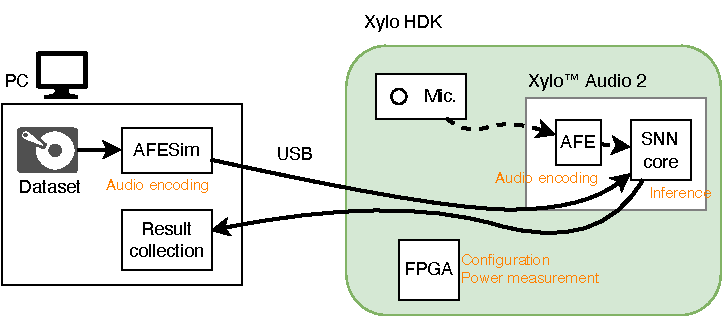
\includegraphics[width=\linewidth]{figures/xylo_system_overview.pdf}
    \vspace*{1cm}
    \end{subfigure}
    \hspace*{0.5cm}
    \begin{subfigure}{0.3\textwidth}
        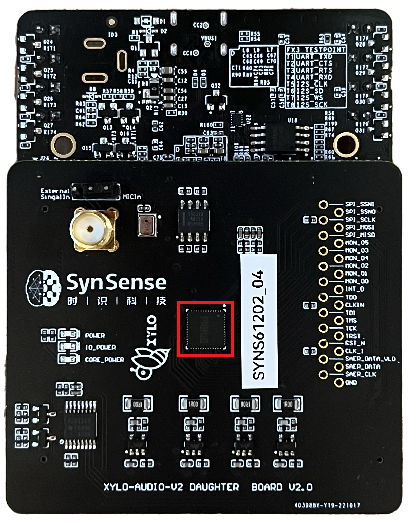
\includegraphics[width=\linewidth]{figures/xyloa2_hdk_fig.pdf}
    \end{subfigure}
        \caption{\secondrev{Left: An overview of the benchmarking system for the Xylo. A simulator of the analog encoding module is run on a PC and streamed to the SNN inference core via USB. After inference, outputs are routed back to the PC for classification. An on-board FPGA configures and records power of the Xylo components. Right: The Xylo\texttrademark Audio 2 hardware development kit (HDK), used as the SUT. The red outline marks the Xylo inference module. Figures taken, with permission, from Ke et al.~\cite{ke2024neurobenchdcase2020acoustic}}}
        \label{fig:xylo}
\end{figure}


\secondrev{\paragraph{CPU} The CPU baseline uses an Arduino Nano 33 BLE board, which runs preprocessing and inference on an ARM Cortex-M4F microcontroller running at 64MHz. All training and deployment uses Edge Impulse, a commercially developed ML-operations platform for tinyML~\cite{hymel2023edgeimpulsemlopsplatform}. The 1 second digital audio samples were converted into two-dimensional frames of Mel-filterbank energies (MFE), and inference uses a network with two convolution layers with batch normalization and max pooling. The trained model was quantized then compiled to an Arduino library using Edge Impulse EON compiler, which optimizes for memory and flash usage. Execution time is measured using on-chip timers from the Arduino, while power is measured using an external multimeter for total system power. Power was measured separately for idle, active pre-processing, and active inference by taking the average power over 60 seconds. The Arduino repeatedly computes over one sample loaded in memory, with a recording frequency of 3 Hz on a Keysight 34465A digital multimeter.}

\secondrev{\paragraph{Synsense Xylo} As shown in Figure~\ref{fig:xylo}, the Xylo baseline used a host PC to run a simulation of the analog pre-processing unit on the benchmark dataset, which was routed into the SNN core on the Xylo SUT. Accuracy is measured by performing a maximum on the output spikes of the SNN. The SNN on Xylo is a feedforward network with three hidden layers, where each layer is connected by synapses with varying time delays. Training is done using the open-source Rockpool toolchain~\cite{rockpool2019}. In order to amortize measurement overheads, power and execution time are measured over continuous streams of 10 seconds of audio, where the execution time result is divided by 10 and the power result is averaged over the duration. The measurements are made by the on-board FPGA, which operates at 12.5MHz and samples power at 1280 Hz. Accuracy is still measured on the 1-second samples. Full details are available in Ke et al.~\cite{ke2024neurobenchdcase2020acoustic}}


\subsubsection*{Quadratic Unconstrained Binary Optimization (QUBO)}
\begin{figure}[t]
    \centering
        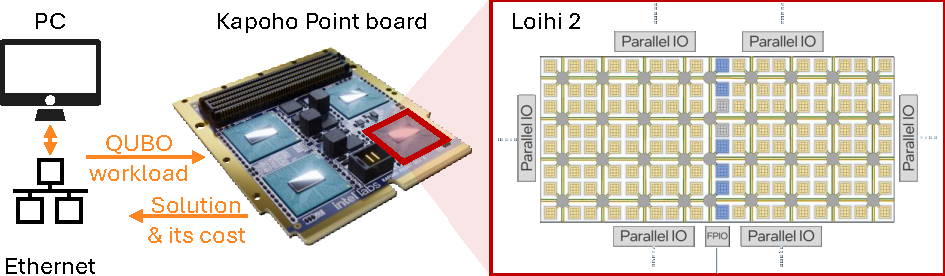
\includegraphics[width=0.85\linewidth]{figures/Loihi2_Benchmarking.pdf}
        \caption{\secondrev{A Kapoho Point board with Loihi 2 chips is connected to a host PC via ethernet. Shown here is a Kapoho Point board with 8 Loihi 2 chips, while the experiments were run on a board with 1 Loihi 2 chip. The QUBO workload is loaded onto the chip, and all processing happens on Loihi 2. On Loihi 2, the neuro-cores, in yellow, are arranged in two $8\times{}8$ grids and iteratively update the variables of the QUBO workload. Embedded CPUs, shown in blue, monitor the cost of the variable assignment. Six parallel IO ports enable 3D stacking of multiple chips for larger workloads than used here. An additional IO port provides the communication to the host PC. The energy and runtime measurements cover the computation of the Loihi 2 chip.}}
        \label{fig:loihi2}
\end{figure}


\secondrev{The processors ran repeatedly with five different initial variable assignments and seeds for different timeouts between $10^{-3}$ s to $10^{3}$ s, and for different workloads sizes of up to $1000$ variables. The neuromorphic algorithm is a parallelized version of simulated annealing that was running on a Kapoho Point board with one Loihi 2 chip, as shown in Figure~\ref{fig:loihi2}. The Loihi 2 board was controlled using Lava \texttt{0.8.0} and Lava Optimization \texttt{0.3.0}. For comparison with conventional hardware, two solvers were adopted based on simulated annealing and tabu search, as implemented in the D-Wave Samplers \texttt{v1.1.0} library \cite{dwavesamplers}. The library was compiled on Ubuntu \texttt{20.04.6 LTS} with GCC \texttt{9.4.0}  and Python \texttt{3.8.10}. CPU measurements were obtained on a machine with Intel Core i9-7920X CPU @ 2.90 GHz and 128GB of DDR4 RAM, using Intel SoC Watch for Linux OS \texttt{2023.2.0}. All details on the solvers, benchmarking routine, and results have been provided by Pierro et al.~\cite{pierro2024solvingquboloihi2}.
}


% \subsection*{System Track Metric Calculations}

% \TODO{Should move figure into the system track section, and probably delete this section from the Methods section}

% % \TODO{Need to verify this power measurement protocol - is it generally agreeable? I think it should note something about whether this is "wall-power" by power analyzer / power meter, or some internally generated power number. Also, do all submissions need to go through the high-level IR? it should be the goal that we have this tooling to aim for arbitrary workload execution, but it seems like the best performance would be achieved by skipping this and going straight to the low-level representation.}

% The correctness or accuracy metric of the systems is obtained in a partially controlled environment based on different representation levels (i.e., high-level and low-level IR in Figure \ref{fig:alg_system_harness}). The high-level consists of a common representation such as the Neuromorphic Intermediate Representation (NIR)~\cite{nir2023} or Lava~\cite{lava} aiming to unify spatio-temporal graphs describing the neuromorphic models to be deployed. Such high-level IR is then transformed into a more optimized representation (low-level IR) that is specific to the target hardware (e.g., sPyNNaker machine graph~\cite{spynnaker}). The low-level IR does not need to be shared between systems to enable hardware vendors to optimize their corresponding neural compilers and runtime execution environments towards achieving a good performance.  

% Throughput, and latency are relatively straightforward metrics to measure and calculate based on the performance of a given hardware platform. Hence, specific relevance is given to the power measurement protocol, as NeuroBench aims to standardize a fair approach to measure and compare different systems. Such protocol is exemplified for scalable systems as they offer presence in both edge- and server- based categories. However, this can be extrapolated to any other neuromorphic system. 

%     \begin{figure}[ht]
%             \centering
%             
\includegraphics[width=.95\textwidth]{figures/system_types.png}
%             \caption{Types of neuromorphic systems.}
%         \label{fig:system_types}
%     \end{figure}

% As presented in Figure~\ref{fig:system_types}, a neuromorphic system can have a single neuromorphic chip, or thousands of them in multi-chip PCBs connected in server setups. These systems commonly include but are not limited to high-speed links to enable fast connectivity within the mesh of neuromorphic processors, flash or any other external memory (e.g., DDR), built-in communication routers, supporting microcontrollers to manage the board, debugging ports (e.g., STLink, etc.), host ports (e.g., Ethernet, CAN, etc.), and a power management (PM) bus. The PM bus is of relevance for the system track metric calculation as it enables access to power consumed at different levels. The following steps exemplify the power characterization process:

% \begin{enumerate}
%     \item Create an SNN with parameters, weights, input spikes; map (partition) SNN to the target hardware and generate its experiment specification.
%     \item Initialize the target hardware.
%     \item Load the binaries (or equivalent) and parameters to the neuromorphic chip and start its cores to initialize them.
%     \item Load input data from the host to the hardware.
%     \item Execute the experiment on hardware triggered by the host. The experiment on the hardware runs standalone for a pre-defined time. This is the step in which the power is measured.
%     \item Read back the results from hardware to host.
%     \item Post-process the results and provide feedback to the user front end.
% \end{enumerate}

% Besides the previous steps, the following gathers some important aspects to establish a fair power management protocol between systems:

% \begin{itemize}
%     \item The power management bus should be connected to every single chip at the different levels of the system.
%     \item Each level should have a mechanism to reliably measure and report power.
%     \item When measurements rely on internal microcontrollers that are not easily accessible to the user, these should be characterized against controlled environments and disclosed within the submission to guarantee the validity of the readings. In complex systems, such characterization can be made for a single-board and extrapolated to the full scale, as the process is complex for supercomputer scales.
% \end{itemize}

% \subsection*{QUBO System Track Benchmark}
% Quadratic unconstrained binary optimization (QUBO) seeks binary variables

% \begin{equation}
% \mathbf{x} \in {0, 1}^n
% \end{equation}

% which optimize the cost function

% \begin{equation}
% C = \mathbf{x}^T \mathbf{Q} \mathbf{x}\ .
% \end{equation}

% The NeuroBench data set is generated by a workload generator and a set of parameters that specify matrices $\mathbf{Q}$. The set includes different workload sizes from $n=10$ binary variables to beyond 100,000s of variables to scale as NC systems mature. The matrix sparsity impacts the difficulty of the problem and is also provided by NeuroBench. For each size and sparsity, NeuroBench provides a set of random workloads for statistical testing.

% The metrics of the NeuroBench system track benchmark differ from benchmarks like MLPerf because NC systems are often designed to allow trading off not just performance and solution accuracy like ML systems, but also energy consumption. For example, neuromorphic systems can leave some of its cores idle to increase efficiency in trade off for less parallelism and thus reduced performance. In addition, NC systems are just maturating and thus quickly increase the size of supported networks. But the QUBO metrics differ also from other benchmarks of NeuroBench as the ground truth optimal solution of an NP-hard QUBO workload is intractable and cannot be straightforwardly determined by human labelling.

% The metrics of the NeuroBench QUBO benchmark account for these effects. The first metric is the maximum workload size supported, to make the benchmark inclusive to NC systems at all maturity levels. Energy efficiency and speed are the second and third metrics, measured by running multiple workloads of the largest supported workload size on the system without knowledge of the ground truth solution like other benchmarks for NP-hard combinatorial optimization \cite{taillard1993}. For each workload, the system is allowed to run for a specific time, and the cost function and energy consumption are recorded. This process is repeated across a range of timeouts. For each timeout, results are averaged over various random workloads of the same size and sparsity. The average accuracy at different timeouts can then be compared between neuromorphic systems and traditional hardware using paired statistics.  If the neuromorphic system outperforms traditional systems in time-to-solution, its energy consumption is then benchmarked separately at various timeouts. This is done by adjusting the system parameters to enhance energy efficiency, even if it means reducing accuracy. However, accuracy is kept just above iso-optimality compared to traditional hardware.  This approach allows to systematically benchmark the system on its maximum speed and its maximum energy efficiency.

% The neuromorphic system is measured against traditional hardware only on the largest workload size it supports to highlight the scaling benefits of neuromorphic computing. Still, researchers are urged to report numbers for all workload sizes supported by their NC system, to facilitate an inclusive comparison with neuromorphic systems that currently support only smaller problem sizes.

% The workload generator, the parameters specifying the workloads, the precise metrics, and initial state-of-the-art baselines on traditional hardware will be published in an upcoming paper and on GitHub.
\section*{Acknowledgements}

% Not compulsory. Acknowledgements should be brief, and should not include thanks to anonymous referees and editors, or effusive comments. Grant or contribution numbers may be acknowledged.

% \TODO{Following seems effusive, should pare it down}
% The NeuroBench project represents a collaborative and inclusive effort, wherein contributions from a diverse group of researchers from both academia and industry have been instrumental in shaping the benchmark design and motivating its release. The authors listed in this paper are only a small subset of the larger community whose collective expertise and dedication have been integral to the development of the NeuroBench initiative. Our project also builds off prior efforts and collaborations from Telluride, Capo Caccia, and NICE, which have driven the NeuroBench community development and trailblazed paths towards inclusive benchmark design. We are immensely grateful to the NeuroBench community for their wisdom, effort, and passion, which they have shared with us in the form of countless meetings, research publications, and other forms of engagement. Without their support and input, NeuroBench would not have been matured from concept to a full-scale community-driven effort, and we look forward to continued collaboration with the community in the evolution of the project.

This work has been supported in parts by Semiconductor Research Corporation (SRC), the European Research Council (ERC) under the European Union’s Horizon 2020 research and innovation programme (grant agreement No.~101001448), a grant from the Research Grants Council of the Hong Kong Special Administrative Region, China [Project No.~CityU 11200922], ARC Laureate Fellowship FL210100156,  and the EU H2020 project BeFerroSynaptic (871737). We acknowledge the financial support of the CogniGron research center and the Ubbo Emmius Funds (Univ. of Groningen). We acknowledge a contribution from the Italian National Recovery and Resilience Plan (NRRP), M4C2, funded by the European Union –NextGenerationEU (Project IR0000011, CUP B51E22000150006, “EBRAINS-Italy”). The work of SynSense was partially supported by the European Commission, under the Horizon grant Ferro4Edge AI (grant agreement 101135656).This work is partly funded by the German Federal Ministry of Education and Research (BMBF) and the free state of Saxony within the ScaDS.AI center of excellence for AI research and by the German Federal Ministry for Economic Affairs and Climate Action (BMWK) under contract 01MN23004F (ESCADE).

Sandia National Laboratories is a multi-mission laboratory managed and operated by National Technology \& Engineering Solutions of Sandia, LLC (NTESS), a wholly owned subsidiary of Honeywell International Inc., for the U.S. Department of Energy’s National Nuclear Security Administration (DOE/NNSA) under contract DE-NA0003525. This written work is authored by an employee of NTESS. The employee, not NTESS, owns the right, title and interest in and to the written work and is responsible for its contents. Any subjective views or opinions that might be expressed in the written work do not necessarily represent the views of the U.S. Government. The publisher acknowledges that the U.S. Government retains a non-exclusive, paid-up, irrevocable, world-wide license to publish or reproduce the published form of this written work or allow others to do so, for U.S. Government purposes. The DOE will provide public access to results of federally sponsored research in accordance with the DOE Public Access Plan. This paper describes objective technical results and analysis. Any subjective views or opinions that might be expressed in the paper do not necessarily represent the views of the U.S. Department of Energy or the United States Government.

\section*{Author contributions statement}
Authors are grouped based on contributions, and ordered alphabetically within groups.
JY led project discussions and management. JY and KVdB implemented harness metric infrastructure, conducted experiments, and prepared the manuscript.
The following authors primarily developed the main algorithm track results: DdB and MF on the keyword few-shot class-incremental learning task; GT and SW on the event camera object detection task; PH, PVS and BZ on the non-human primate motor prediction task; YB and DK on the chaotic function prediction task; and NP led harness infrastructure development. The following authors primarily developed the main system track results: WK and MAK on the acoustic scene classification task; AP and PS on the QUBO task.
SHA, GVJ, BL, AM, AKM, GL, and TS developed components of the algorithm track harness infrastructure.
ZA, MA, BA, AGA, CB, AB, PB, SB, SB, GC, EC, FC, GdC, AD, AD, MD, YD, JE, TF, JF, VF, SF, PMF, WG, AG, HAG, GI, SJ, VK, LK, JCK, LK, RK, DK, YL, SL, HM, RM, FMM, CM, KM, DRM, EN, TN, FO, AO, PP, JP, MP, CP, MAP, CP, AR, YS, CJSS, AvS, JS, SS, CS, JS, SS, SBS, MS, AS, MS, KS, TCS, JT, NT, GU, MV, CMV, BV, AY, and FTZ participated in discussions during meetings, prepared sections for the present manuscript and/or its preprint, and reviewed the manuscript.
CF and VJR jointly supervised the project, reviewed the manuscript, and analyzed results.

% Must include all authors, identified by initials, for example:
% A.A. conceived the experiment(s),  A.A. and B.A. conducted the experiment(s), C.A. and D.A. analysed the results.  All authors reviewed the manuscript. 

\bibliography{ref}

% To include, in this order: \textbf{Accession codes} (where applicable); \textbf{Competing interests} (mandatory statement). 

\section*{Additional information}

\subsection*{Competing interests statement}
% The corresponding author is responsible for submitting a \href{http://www.nature.com/srep/policies/index.html#competing}{competing interests statement} on behalf of all authors of the paper. This statement must be included in the submitted article file.

The NeuroBench benchmark framework was developed collaboratively and specifically to allow for as objective and applicable comparison as possible. The selection of initial benchmark tasks reflect the authors' research interests, which includes commercial interests for companies. These do not affect our results in any way, nor the value of our contributions. The benchmark harness and framework are open-source and intended to be further extended by the community over time.

% Initial benchmark tasks and baselines reflect the authors' research interests, however the open-source benchmark harness and framework itself are meant to be extended by the community over time.

%%%      %%%

\end{document}